% Options for packages loaded elsewhere
\PassOptionsToPackage{unicode}{hyperref}
\PassOptionsToPackage{hyphens}{url}
%
\documentclass[
]{book}
\usepackage{amsmath,amssymb}
\usepackage{iftex}
\ifPDFTeX
  \usepackage[T1]{fontenc}
  \usepackage[utf8]{inputenc}
  \usepackage{textcomp} % provide euro and other symbols
\else % if luatex or xetex
  \usepackage{unicode-math} % this also loads fontspec
  \defaultfontfeatures{Scale=MatchLowercase}
  \defaultfontfeatures[\rmfamily]{Ligatures=TeX,Scale=1}
\fi
\usepackage{lmodern}
\ifPDFTeX\else
  % xetex/luatex font selection
\fi
% Use upquote if available, for straight quotes in verbatim environments
\IfFileExists{upquote.sty}{\usepackage{upquote}}{}
\IfFileExists{microtype.sty}{% use microtype if available
  \usepackage[]{microtype}
  \UseMicrotypeSet[protrusion]{basicmath} % disable protrusion for tt fonts
}{}
\makeatletter
\@ifundefined{KOMAClassName}{% if non-KOMA class
  \IfFileExists{parskip.sty}{%
    \usepackage{parskip}
  }{% else
    \setlength{\parindent}{0pt}
    \setlength{\parskip}{6pt plus 2pt minus 1pt}}
}{% if KOMA class
  \KOMAoptions{parskip=half}}
\makeatother
\usepackage{xcolor}
\usepackage{color}
\usepackage{fancyvrb}
\newcommand{\VerbBar}{|}
\newcommand{\VERB}{\Verb[commandchars=\\\{\}]}
\DefineVerbatimEnvironment{Highlighting}{Verbatim}{commandchars=\\\{\}}
% Add ',fontsize=\small' for more characters per line
\usepackage{framed}
\definecolor{shadecolor}{RGB}{248,248,248}
\newenvironment{Shaded}{\begin{snugshade}}{\end{snugshade}}
\newcommand{\AlertTok}[1]{\textcolor[rgb]{0.94,0.16,0.16}{#1}}
\newcommand{\AnnotationTok}[1]{\textcolor[rgb]{0.56,0.35,0.01}{\textbf{\textit{#1}}}}
\newcommand{\AttributeTok}[1]{\textcolor[rgb]{0.13,0.29,0.53}{#1}}
\newcommand{\BaseNTok}[1]{\textcolor[rgb]{0.00,0.00,0.81}{#1}}
\newcommand{\BuiltInTok}[1]{#1}
\newcommand{\CharTok}[1]{\textcolor[rgb]{0.31,0.60,0.02}{#1}}
\newcommand{\CommentTok}[1]{\textcolor[rgb]{0.56,0.35,0.01}{\textit{#1}}}
\newcommand{\CommentVarTok}[1]{\textcolor[rgb]{0.56,0.35,0.01}{\textbf{\textit{#1}}}}
\newcommand{\ConstantTok}[1]{\textcolor[rgb]{0.56,0.35,0.01}{#1}}
\newcommand{\ControlFlowTok}[1]{\textcolor[rgb]{0.13,0.29,0.53}{\textbf{#1}}}
\newcommand{\DataTypeTok}[1]{\textcolor[rgb]{0.13,0.29,0.53}{#1}}
\newcommand{\DecValTok}[1]{\textcolor[rgb]{0.00,0.00,0.81}{#1}}
\newcommand{\DocumentationTok}[1]{\textcolor[rgb]{0.56,0.35,0.01}{\textbf{\textit{#1}}}}
\newcommand{\ErrorTok}[1]{\textcolor[rgb]{0.64,0.00,0.00}{\textbf{#1}}}
\newcommand{\ExtensionTok}[1]{#1}
\newcommand{\FloatTok}[1]{\textcolor[rgb]{0.00,0.00,0.81}{#1}}
\newcommand{\FunctionTok}[1]{\textcolor[rgb]{0.13,0.29,0.53}{\textbf{#1}}}
\newcommand{\ImportTok}[1]{#1}
\newcommand{\InformationTok}[1]{\textcolor[rgb]{0.56,0.35,0.01}{\textbf{\textit{#1}}}}
\newcommand{\KeywordTok}[1]{\textcolor[rgb]{0.13,0.29,0.53}{\textbf{#1}}}
\newcommand{\NormalTok}[1]{#1}
\newcommand{\OperatorTok}[1]{\textcolor[rgb]{0.81,0.36,0.00}{\textbf{#1}}}
\newcommand{\OtherTok}[1]{\textcolor[rgb]{0.56,0.35,0.01}{#1}}
\newcommand{\PreprocessorTok}[1]{\textcolor[rgb]{0.56,0.35,0.01}{\textit{#1}}}
\newcommand{\RegionMarkerTok}[1]{#1}
\newcommand{\SpecialCharTok}[1]{\textcolor[rgb]{0.81,0.36,0.00}{\textbf{#1}}}
\newcommand{\SpecialStringTok}[1]{\textcolor[rgb]{0.31,0.60,0.02}{#1}}
\newcommand{\StringTok}[1]{\textcolor[rgb]{0.31,0.60,0.02}{#1}}
\newcommand{\VariableTok}[1]{\textcolor[rgb]{0.00,0.00,0.00}{#1}}
\newcommand{\VerbatimStringTok}[1]{\textcolor[rgb]{0.31,0.60,0.02}{#1}}
\newcommand{\WarningTok}[1]{\textcolor[rgb]{0.56,0.35,0.01}{\textbf{\textit{#1}}}}
\usepackage{longtable,booktabs,array}
\usepackage{calc} % for calculating minipage widths
% Correct order of tables after \paragraph or \subparagraph
\usepackage{etoolbox}
\makeatletter
\patchcmd\longtable{\par}{\if@noskipsec\mbox{}\fi\par}{}{}
\makeatother
% Allow footnotes in longtable head/foot
\IfFileExists{footnotehyper.sty}{\usepackage{footnotehyper}}{\usepackage{footnote}}
\makesavenoteenv{longtable}
\usepackage{graphicx}
\makeatletter
\def\maxwidth{\ifdim\Gin@nat@width>\linewidth\linewidth\else\Gin@nat@width\fi}
\def\maxheight{\ifdim\Gin@nat@height>\textheight\textheight\else\Gin@nat@height\fi}
\makeatother
% Scale images if necessary, so that they will not overflow the page
% margins by default, and it is still possible to overwrite the defaults
% using explicit options in \includegraphics[width, height, ...]{}
\setkeys{Gin}{width=\maxwidth,height=\maxheight,keepaspectratio}
% Set default figure placement to htbp
\makeatletter
\def\fps@figure{htbp}
\makeatother
\usepackage{soul}
\setlength{\emergencystretch}{3em} % prevent overfull lines
\providecommand{\tightlist}{%
  \setlength{\itemsep}{0pt}\setlength{\parskip}{0pt}}
\setcounter{secnumdepth}{5}
\usepackage{booktabs}
\ifLuaTeX
  \usepackage{selnolig}  % disable illegal ligatures
\fi
\usepackage[]{natbib}
\bibliographystyle{plainnat}
\IfFileExists{bookmark.sty}{\usepackage{bookmark}}{\usepackage{hyperref}}
\IfFileExists{xurl.sty}{\usepackage{xurl}}{} % add URL line breaks if available
\urlstyle{same}
\hypersetup{
  pdftitle={A Minimal Book Example},
  pdfauthor={John Doe},
  hidelinks,
  pdfcreator={LaTeX via pandoc}}

\title{A Minimal Book Example}
\author{John Doe}
\date{2023-07-14}

\usepackage{amsthm}
\newtheorem{theorem}{Theorem}[chapter]
\newtheorem{lemma}{Lemma}[chapter]
\newtheorem{corollary}{Corollary}[chapter]
\newtheorem{proposition}{Proposition}[chapter]
\newtheorem{conjecture}{Conjecture}[chapter]
\theoremstyle{definition}
\newtheorem{definition}{Definition}[chapter]
\theoremstyle{definition}
\newtheorem{example}{Example}[chapter]
\theoremstyle{definition}
\newtheorem{exercise}{Exercise}[chapter]
\theoremstyle{definition}
\newtheorem{hypothesis}{Hypothesis}[chapter]
\theoremstyle{remark}
\newtheorem*{remark}{Remark}
\newtheorem*{solution}{Solution}
\begin{document}
\maketitle

{
\setcounter{tocdepth}{1}
\tableofcontents
}
\hypertarget{about}{%
\chapter{About}\label{about}}

This is a \emph{sample} book written in \textbf{Markdown}. You can use anything that Pandoc's Markdown supports; for example, a math equation \(a^2 + b^2 = c^2\).

\hypertarget{usage}{%
\section{Usage}\label{usage}}

Each \textbf{bookdown} chapter is an .Rmd file, and each .Rmd file can contain one (and only one) chapter. A chapter \emph{must} start with a first-level heading: \texttt{\#\ A\ good\ chapter}, and can contain one (and only one) first-level heading.

Use second-level and higher headings within chapters like: \texttt{\#\#\ A\ short\ section} or \texttt{\#\#\#\ An\ even\ shorter\ section}.

The \texttt{index.Rmd} file is required, and is also your first book chapter. It will be the homepage when you render the book.

\hypertarget{render-book}{%
\section{Render book}\label{render-book}}

You can render the HTML version of this example book without changing anything:

\begin{enumerate}
\def\labelenumi{\arabic{enumi}.}
\item
  Find the \textbf{Build} pane in the RStudio IDE, and
\item
  Click on \textbf{Build Book}, then select your output format, or select ``All formats'' if you'd like to use multiple formats from the same book source files.
\end{enumerate}

Or build the book from the R console:

\begin{Shaded}
\begin{Highlighting}[]
\NormalTok{bookdown}\SpecialCharTok{::}\FunctionTok{render\_book}\NormalTok{()}
\end{Highlighting}
\end{Shaded}

To render this example to PDF as a \texttt{bookdown::pdf\_book}, you'll need to install XeLaTeX. You are recommended to install TinyTeX (which includes XeLaTeX): \url{https://yihui.org/tinytex/}.

\hypertarget{preview-book}{%
\section{Preview book}\label{preview-book}}

As you work, you may start a local server to live preview this HTML book. This preview will update as you edit the book when you save individual .Rmd files. You can start the server in a work session by using the RStudio add-in ``Preview book'', or from the R console:

\begin{Shaded}
\begin{Highlighting}[]
\NormalTok{bookdown}\SpecialCharTok{::}\FunctionTok{serve\_book}\NormalTok{()}
\end{Highlighting}
\end{Shaded}

\hypertarget{ux43dux430ux447ux430ux43bux43e-ux440ux430ux431ux43eux442ux44b-ux441-r}{%
\chapter{Начало работы с R}\label{ux43dux430ux447ux430ux43bux43e-ux440ux430ux431ux43eux442ux44b-ux441-r}}

\hypertarget{ux447ux442ux43e-ux442ux430ux43aux43eux435-r}{%
\section{Что такое R?}\label{ux447ux442ux43e-ux442ux430ux43aux43eux435-r}}

R --- это язык программирования для статистической обработки данных и работы с графикой. Он создан в 90-х гг. на факультете статистики Оклендского университета. Иными словами, его делали статистики и для статистиков. Поэтому он прекрасно подходит для анализа данных, статистических вычислений и машинного обучения, а значит востребован в науке.

\begin{quote}
Язык R --- один из самых распространённых в научной среде. Им пользуются математики, биологи, генетики и другие учёные, которым нужно проводить статистические исследования и строить модели. Поэтому язык R нужно изучать тем, кто планирует заниматься научными исследованиями.

--- Яндекс Практикум \href{https://practicum.yandex.ru/blog/chto-takoe-yazyk-r/\#chto-takoe}{Блог}
\end{quote}

После установки R вы получите доступ к уже готовым методам статистического анализа и инструментам для визуализации. Но за счет того, что R распространяется свободно, постоянно появляются новые алгоритмы, созданные внутри экспертного сообщества и тоже доступные для всех. Как и любой язык, R растет и развивается.

\hypertarget{ux43fux430ux43aux435ux442ux44b-ux438-ux432ux438ux43dux44cux435ux442ux43aux438}{%
\section{Пакеты и виньетки}\label{ux43fux430ux43aux435ux442ux44b-ux438-ux432ux438ux43dux44cux435ux442ux43aux438}}

Если в базовой инсталляции R нет нужного решения -- имеет смысл поискать в библиотеке \textbf{пакетов}. Пакет -- это \textbf{набор функций} и иногда датасетов, созданный пользователями. На 1 июля 2023 г. в репозитории \href{https://cran.r-project.org/}{CRAN} доступно 19789 пакетов. И это далеко не все: многие пакеты доступны только на GitHub, например \href{https://rdrr.io/github/dracor-org/rdracor/f/README.md}{пакет Dracor}, к которому я буду обращаться в рамках этого курса.

Некоторые функции, которые вы найдете в пакетах, частично дублируют друг друга -- это нормально, как и в естественном языке, ``сказать'' что-то можно разными способами.

Несмотря на то, что R создавался изначально для работы со статистикой, система свободно распространяемых модулей значительно расширяет круг задач, которые можно решать на этом языке. Например, благодаря модулю Shiny можно создавать \href{https://locusclassicus.shinyapps.io/myshinyapp/}{приложения} и встраивать их в веб-страницы, а модуль Leaflet позволяет создавать интерактивные карты. \href{http://antibarbari.ru/2023/03/01/cicero_villas/}{Одну из них} мы сделали в рамках проекта Antibarbari HSE. В рамках этого курса мы познакомимся и с модулями для машинного обучения. Нейросети в R тоже можно строить, но мы пока не будем.

По технической документации и так называемым ``виньеткам'' можно понять, какой пакет вам нужен. Например, вот так выглядит \href{https://docs.ropensci.org/rperseus/articles/rperseus-vignette.html}{виньетка} пакета \texttt{RPerseus}, при помощи которого можно получить доступ к корпусу греческой и латинской литературы.

Бывают еще \textbf{``пакеты пакетов''}, то есть очень большие семейства функций, своего рода ``диалекты'' R. Таково, например, семейство \texttt{tidyverse}, объединяемое идеологией ``опрятных'' данных. Про него мы еще будем говорить.

\hypertarget{ux435ux441ux43bux438-ux43dux435-ux445ux432ux430ux442ux430ux435ux442-ux43fux430ux43aux435ux442ux43eux432}{%
\section{Если не хватает пакетов}\label{ux435ux441ux43bux438-ux43dux435-ux445ux432ux430ux442ux430ux435ux442-ux43fux430ux43aux435ux442ux43eux432}}

Это самое интересное. Если вы работаете в программе с графическим интерфейсом (SPSS, Minitab), то вы вынуждены формулировать свою задачу так, чтобы ``вписаться'' в набор кнопок, предусмотренных разработчиком. В R, столкнувшись с особой задачей, вы просто пишете под нее особую функцию.

Новую функцию не обязательно публиковать в составе пакета -- можно сохранить в рабочую директорию (с расширением \texttt{.R}) и наслаждаться самому. По мере того, как развиваются ваши навыки программирования, вы можете ставить и решать все более сложные и интересные задачи.

\hypertarget{ux43e-ux432ux43eux441ux43fux440ux43eux438ux437ux432ux43eux434ux438ux43cux43eux441ux442ux438}{%
\section{О воспроизводимости}\label{ux43e-ux432ux43eux441ux43fux440ux43eux438ux437ux432ux43eux434ux438ux43cux43eux441ux442ux438}}

Когда вы решите опубликовать свое исследование, то и код к нему придется опубликовать (как правило, для этого используется GitHub) -- поэтому надо сразу привыкать кодить так, чтобы ваш код был понятен другим. Например, добавлять пояснения при помощи знака \texttt{\#} (как в Python)

\begin{Shaded}
\begin{Highlighting}[]
\CommentTok{\# случайный набор чисел из нормального распределения}
\NormalTok{x }\OtherTok{\textless{}{-}} \FunctionTok{rnorm}\NormalTok{(}\DecValTok{1000}\NormalTok{)}
\CommentTok{\# случайная выборка из этого набора}
\NormalTok{y }\OtherTok{\textless{}{-}} \FunctionTok{sample}\NormalTok{(x, }\DecValTok{100}\NormalTok{)}
\end{Highlighting}
\end{Shaded}

В идеале, впрочем, вы поясняете не то, \emph{что} код делает (при грамотном кодинге это должно быть самоочевидо), а \emph{зачем}.

В этом примере код, правда, настолько простой, что не требует особых пояснений. Но в больших проектах от ``читабельности'' кода зависит не только то, поймет ли вас потенциальный рецензент, но и сможете ли вы сами вспомнить, какая строчка за что отвечает. Также это позволит вернуться к проекту через некоторое время и быстро вспомнить, что там происходит.

Если вы получите интересные результаты и решите их опубликовать, то выложить в открытый доступ придется не только код, но и данные (если они не защищены копирайтом или другими ограничениями). Таким образом рецензент или другие ученые, которые будут читать вашу статью, сможет перепроверить ваши выводы. Ученые так делают!

И это еще один довод в пользу того, чтобы научиться программировать, а не полагаться на ПО с графическим интерфейсом.

\hypertarget{ux447ux442ux43e-ux43cux44b-ux43dux435-ux431ux443ux434ux435ux43c-ux434ux435ux43bux430ux442ux44c}{%
\section{Что мы (не) будем делать?}\label{ux447ux442ux43e-ux43cux44b-ux43dux435-ux431ux443ux434ux435ux43c-ux434ux435ux43bux430ux442ux44c}}

Хотя возможности R очень широки, мы будем заниматься в основном анализом текстовых данных. ``Текст'' в данном случае можно понимать как зафиксированную (в машиночитаемом виде) речь: от отзыва на товар до романа. Но в основном данные я подбираю таким образом, чтобы они были интересны гуманитариям.

Мы \emph{не будем} анализировать звучащую речь (хотя это тоже \href{https://ling.hse.ru/news/671710245.html}{можно делать} в R). И мы не будем заниматься распознаванием рукописных символов, для этого есть гораздо другие \href{https://vk.com/video-211800158_456239315}{мощные инструменты}. Веб-скрапинг и нейронные сети тоже не входят в число тем этого курса.

Курс включает в себя три основных блока и 24 урока:

\begin{itemize}
\tightlist
\item
  общее введение в R (темы 1-6)
\item
  text-mining (темы 7-13)
\item
  статистика и статистическое обучение (14-22)
\end{itemize}

Еще два урока посвящены модулям Plotly и Leaflet.

Если вы плохо представляете, на что вообще способны количественные методы в гуманитаристике, посмотрите видео панельной дискуссии \href{https://vk.com/video-211800158_456239307}{``Цифровые инструменты и методы: в чем их польза и как им обучить гуманитария?''} (НИУ ВШЭ, 2023 г.). Это видео о том, зачем. О том, как -- дальше.

\hypertarget{rstudio}{%
\section{RStudio}\label{rstudio}}

Работать в R мы будем с использованием RStudio, которая представляет собой свободную среду разработки (IDE) программного обеспечения с открытым исходным кодом для языка программирования R.

Наша задача в этом уроке -- установить R и R Studio и убедиться, что все работает; научиться самостоятельно находить помощь, совершать несложные вычисления.

\hypertarget{ux443ux441ux442ux430ux43dux43eux432ux43aux430}{%
\section{Установка}\label{ux443ux441ux442ux430ux43dux43eux432ux43aux430}}

\begin{enumerate}
\def\labelenumi{\arabic{enumi}.}
\tightlist
\item
  Установить R
\end{enumerate}

\begin{itemize}
\tightlist
\item
  Скачать R для Windows: \url{https://cran.r-project.org/bin/windows/}
\item
  Скачать R для Mac: \url{https://cran.r-project.org/bin/macosx/}
\end{itemize}

\begin{enumerate}
\def\labelenumi{\arabic{enumi}.}
\setcounter{enumi}{1}
\tightlist
\item
  Установить R Studio
\end{enumerate}

\begin{itemize}
\tightlist
\item
  Скачать: \url{https://www.rstudio.com/products/rstudio/download/} (достаточно бесплатной версии)
\end{itemize}

На MacOS для работы библиотеки Stylo также понадобится установить XQuartz: \url{https://www.xquartz.org/}

\hypertarget{ux43dux430ux447ux430ux43bux43e-ux440ux430ux431ux43eux442ux44b}{%
\section{Начало работы}\label{ux43dux430ux447ux430ux43bux43e-ux440ux430ux431ux43eux442ux44b}}

После установки и запуска RStudio вы увидите вот такие четыре панели (их названия подписаны на картинке):

\begin{figure}
\centering
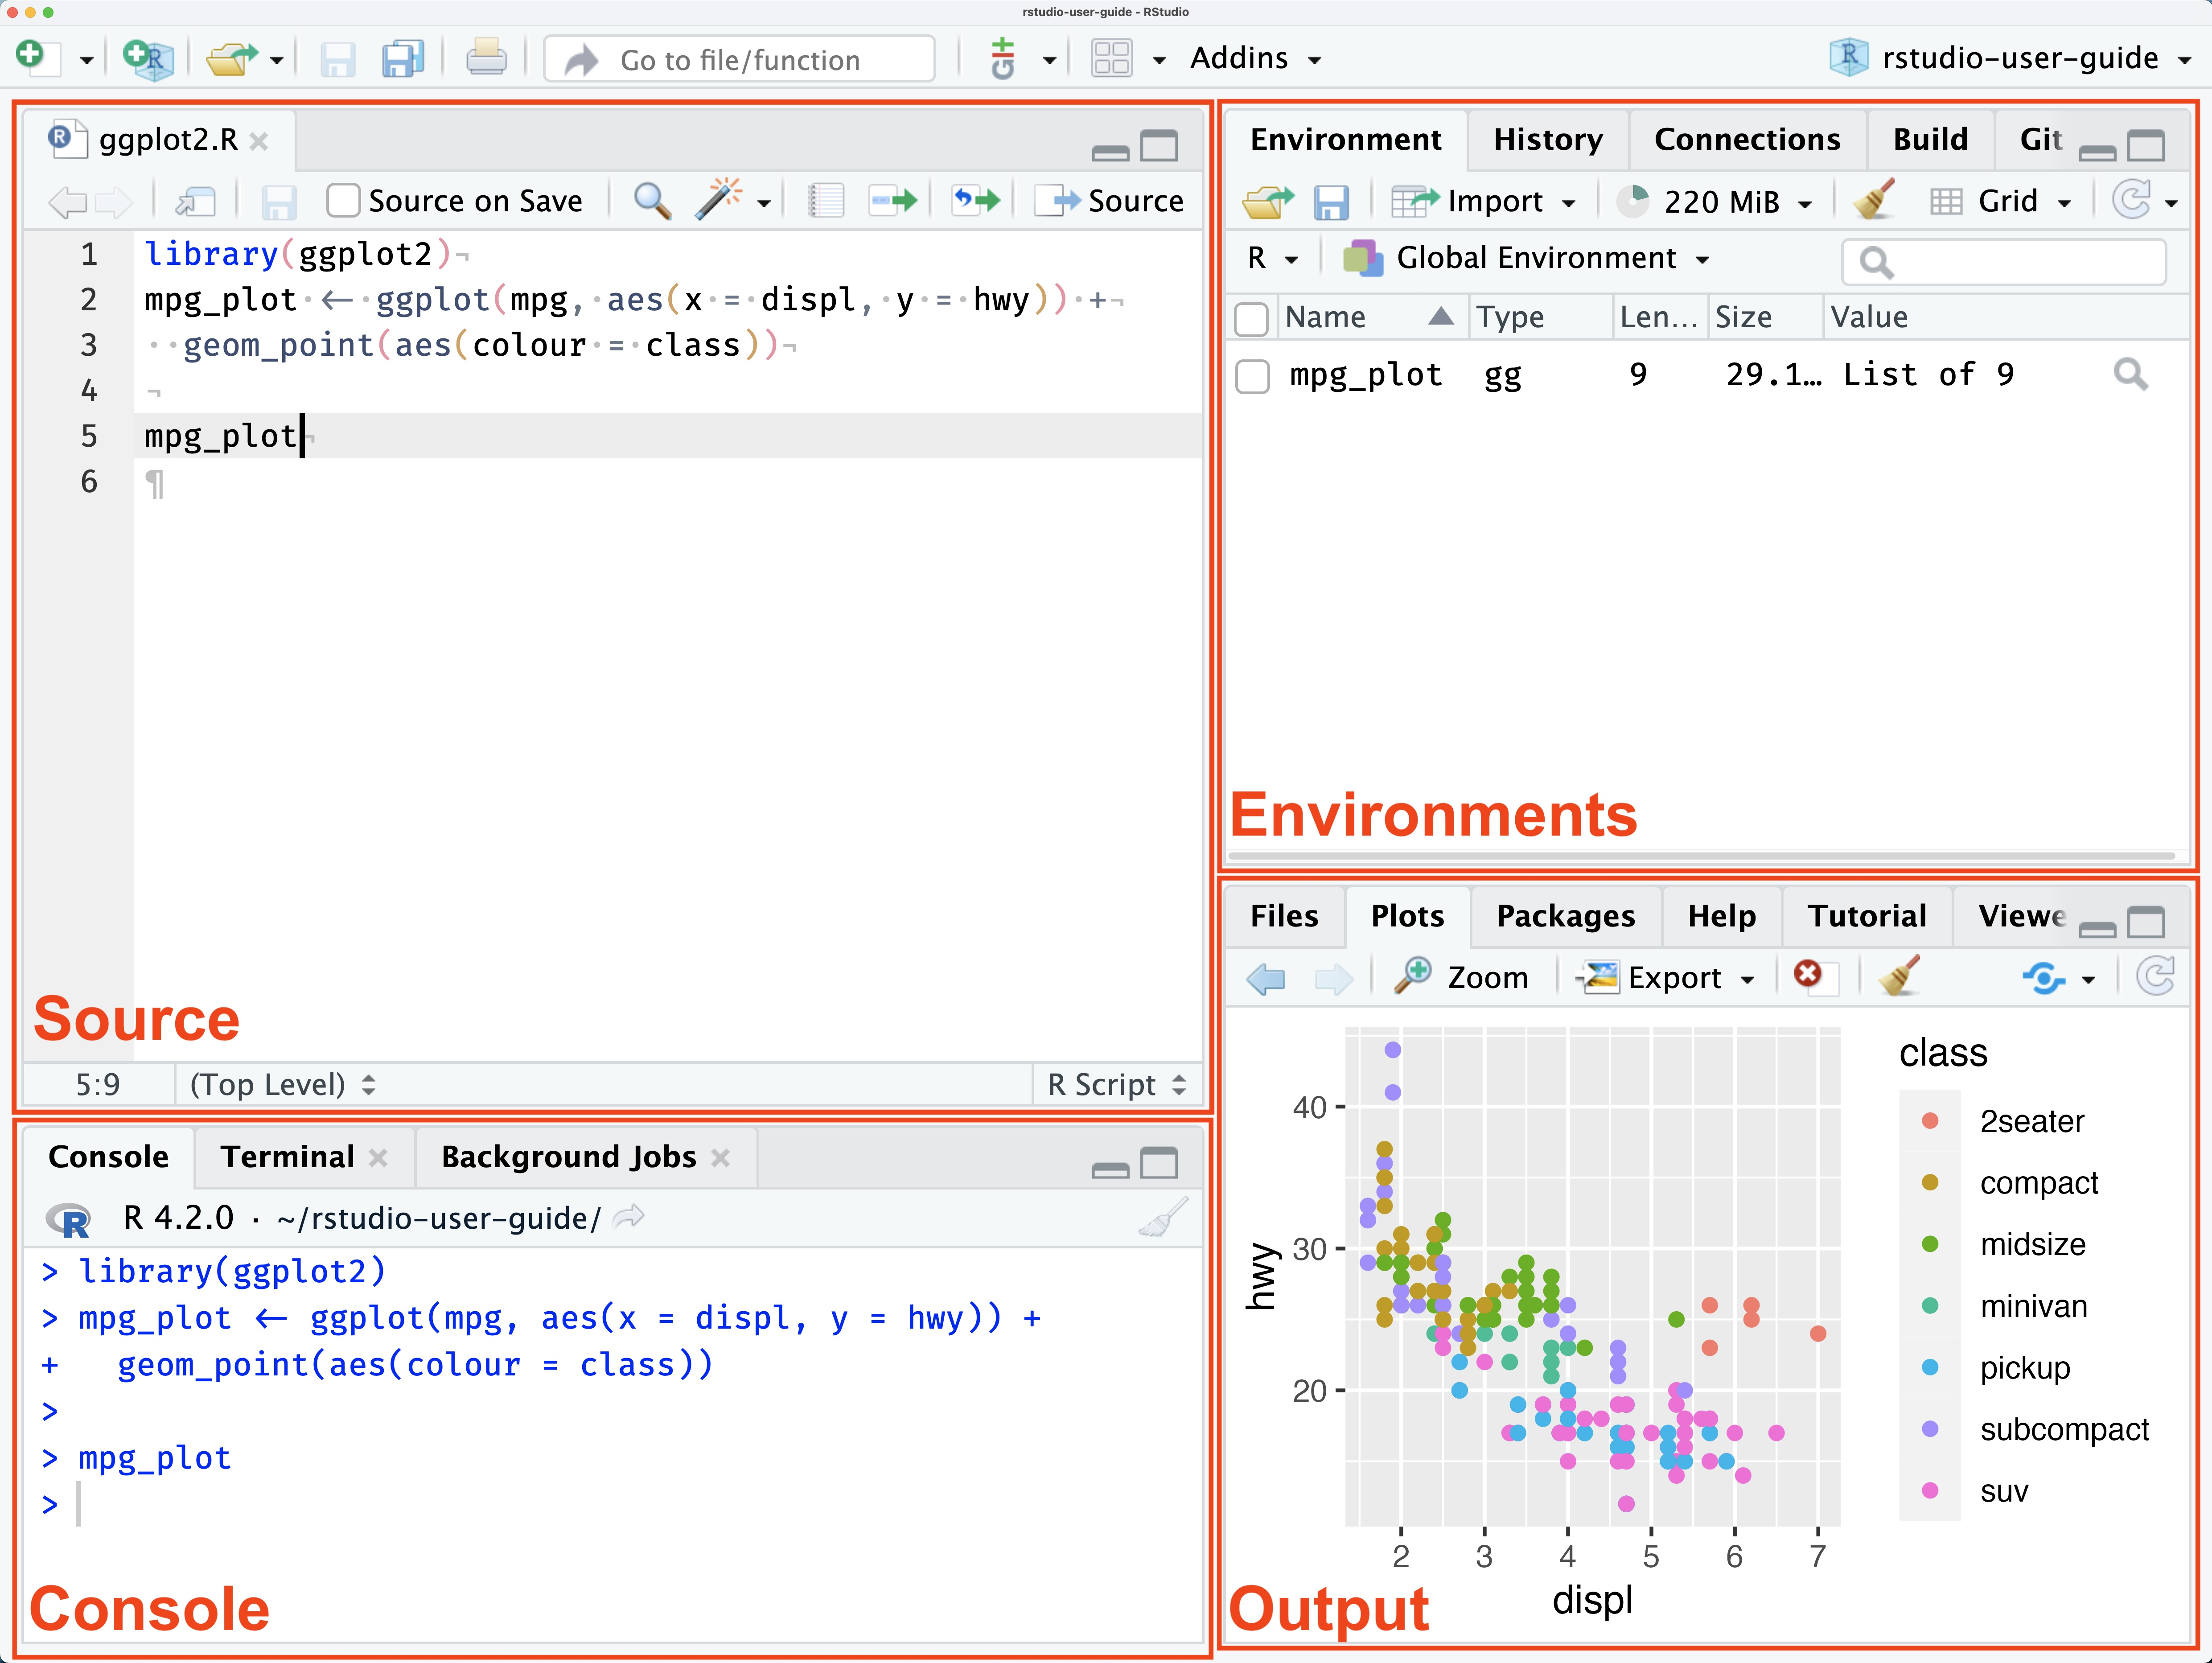
\includegraphics{images/panes.jpeg}
\caption{RStudio Panes}
\end{figure}

По \href{https://docs.posit.co/ide/user/ide/guide/ui/ui-panes.html}{ссылке} можно подробнее прочитать, что за что отвечает (и как это поменять).

Для начала попробуйте получить информацию о сессии, введя в \textbf{консоли} такую команду:

\begin{Shaded}
\begin{Highlighting}[]
\FunctionTok{sessionInfo}\NormalTok{()}
\end{Highlighting}
\end{Shaded}

\texttt{sessionInfo()} -- это \textbf{функция}. За названием функции всегда следуют круглые скобки, внутри которых могут находиться \textbf{аргументы функции}. О функциях можно думать как о глаголах (``сделай то-то!''). Аргументы -- это что-то вроде дополнений и обстоятельств. (Кстати, в ``диалекте'' tidyverse есть функции-наречия, так что аналогия законная.) Аргументы могут быть обязательные и необязательные.

Чтобы узнать, каких аргументов требует функция, надо вызывать \textbf{help}: \texttt{?mean()}. Также можно (и нужно) читать техническую документацию к пакетам.

Уточнить свою \textbf{рабочую директорию} (в которой R будет искать и сохранять файлы) можно при помощи функции \texttt{getwd()} без аргументов. Установить рабочую директорию можно при помощи функции \texttt{setwd()}, указав в качестве аргумента путь к рабочей директории на вашем компьютере (в кавычках, так как это символьный вектор). В моем случае это выглядит так:

\begin{Shaded}
\begin{Highlighting}[]
\FunctionTok{setwd}\NormalTok{(}\StringTok{"/Users/olga/R\_Workflow/"}\NormalTok{)}
\end{Highlighting}
\end{Shaded}

Также для выбора рабочей директории можно использовать меню R \texttt{Session\ \textgreater{}\ Set\ Working\ Directory}.

Пакеты для работы устанавливаются один раз, однако подключать их надо во время каждой сессии. Чтобы установить новый пакет, можно воспользоваться меню \texttt{Tools\ \textgreater{}\ Install\ Packages}. Также можно устанавливать пакеты из консоли. Установим пакет для анализа лингвистических данных:

\begin{Shaded}
\begin{Highlighting}[]
\FunctionTok{install.packages}\NormalTok{(}\StringTok{"languageR"}\NormalTok{)}
\end{Highlighting}
\end{Shaded}

Для подключения используем функцию \texttt{library()}, которой передаем в качестве аргумента название пакета без кавычек:

\begin{Shaded}
\begin{Highlighting}[]
\FunctionTok{library}\NormalTok{(languageR)}
\end{Highlighting}
\end{Shaded}

Что еще надо знать:

\begin{itemize}
\tightlist
\item
  как создавать проекты в R и почему это удобно \footnote{\url{https://intro2r.com/rsprojs.html}}
\item
  как создавать и хранить файлы с кодом
\end{itemize}

\hypertarget{r-ux43aux430ux43a-ux43aux430ux43bux44cux43aux443ux43bux44fux442ux43eux440}{%
\section{R как калькулятор}\label{r-ux43aux430ux43a-ux43aux430ux43bux44cux43aux443ux43bux44fux442ux43eux440}}

Можно использовать . Для этого вводим данные рядом с символом приглашения \texttt{\textgreater{}}, который называется \textbf{prompt}.

\begin{Shaded}
\begin{Highlighting}[]
\FunctionTok{sqrt}\NormalTok{(}\DecValTok{4}\NormalTok{) }\CommentTok{\# квадратный корень}
\end{Highlighting}
\end{Shaded}

\begin{verbatim}
## [1] 2
\end{verbatim}

\begin{Shaded}
\begin{Highlighting}[]
\DecValTok{2}\SpecialCharTok{\^{}}\DecValTok{3} \CommentTok{\# степень}
\end{Highlighting}
\end{Shaded}

\begin{verbatim}
## [1] 8
\end{verbatim}

\begin{Shaded}
\begin{Highlighting}[]
\FunctionTok{log10}\NormalTok{(}\DecValTok{100}\NormalTok{) }\CommentTok{\#логарифм}
\end{Highlighting}
\end{Shaded}

\begin{verbatim}
## [1] 2
\end{verbatim}

Если в начале консольной строки стоит \texttt{+}, значит предыдущий код не завершен. Например, вы забыли закрыть скобку функции. Ее можно дописать на следующей строке. Попробуйте набрать \texttt{sqrt(2} в консоли.

\hypertarget{ux43eux43fux435ux440ux430ux442ux43eux440ux44b-ux43fux440ux438ux441ux432ux430ux438ux432ux430ux43dux438ux44f}{%
\section{Операторы присваивания}\label{ux43eux43fux435ux440ux430ux442ux43eux440ux44b-ux43fux440ux438ux441ux432ux430ux438ux432ux430ux43dux438ux44f}}

Чтобы в окружении появился новый объект, надо присвоить результат вычислений какой-нибудь переменной при помощи \textbf{оператора присваивания} \texttt{\textless{}-} (\texttt{Alt} + \texttt{-} (Windows) или \texttt{Option} + \texttt{-} (Mac)). Знак \texttt{=} также работает как оператор присваивания, но не во всех контекстах, поэтому им лучше не пользоваться.

\begin{Shaded}
\begin{Highlighting}[]
\NormalTok{x }\OtherTok{\textless{}{-}} \DecValTok{2} \SpecialCharTok{+} \DecValTok{2} \CommentTok{\# создаем переменную}
\NormalTok{y }\OtherTok{\textless{}{-}} \FloatTok{0.1} \CommentTok{\# создаем еще одну переменную}
\NormalTok{x }\OtherTok{\textless{}{-}}\NormalTok{ y }\CommentTok{\# переназначаем значение }
\NormalTok{x }\SpecialCharTok{+}\NormalTok{ y}
\end{Highlighting}
\end{Shaded}

\begin{verbatim}
## [1] 0.2
\end{verbatim}

\textbf{Имя переменной}, как и имя функции, может содержать прописные и строчные буквы, точку и знак подчеркивания. Функция \texttt{c()} (concatenation) позволяет собрать несколько элементов в единый вектор:

\begin{Shaded}
\begin{Highlighting}[]
\NormalTok{x }\OtherTok{\textless{}{-}} \FunctionTok{c}\NormalTok{(}\DecValTok{3}\NormalTok{, }\DecValTok{5}\NormalTok{, }\DecValTok{7}\NormalTok{)}
\NormalTok{x\_mean }\OtherTok{\textless{}{-}} \FunctionTok{mean}\NormalTok{(x) }\CommentTok{\# также возможно x.mean или xMean}
\NormalTok{x\_mean}
\end{Highlighting}
\end{Shaded}

\begin{verbatim}
## [1] 5
\end{verbatim}

В диалекте tidyverse предпочтение отдается подчеркиванию, а не точке; здесь сказывается влияние синтаксиса Python, где через точку получают доступ к методам объекта. Будьте внимательны: R чувствительна к регистру!

\textbf{Объекты, предназначенные для хранения данных}, -- это отдельные переменные, векторы, матрицы и массивы, списки, факторы, таблицы данных. \textbf{Функции} -- это поименованные программы, предназначенные для создания новых объектов или выполнения определенных действий над ними \citep[24]{мастицкий2015}

Чтобы получить список всех объектов в окружении, используется функция \texttt{ls()}. Удалять объекты можно при помощи \texttt{rm()}. Функции можно вкладывать друг в друга:

\begin{Shaded}
\begin{Highlighting}[]
\FunctionTok{rm}\NormalTok{(}\AttributeTok{list =} \FunctionTok{ls}\NormalTok{()) }\CommentTok{\# удаляет все объекты в окружении}
\end{Highlighting}
\end{Shaded}

\hypertarget{ux432ux435ux43aux442ux43eux440ux44b}{%
\section{Векторы}\label{ux432ux435ux43aux442ux43eux440ux44b}}

В языке R нет скаляров (отдельных чисел). Числа считаются векторами из одного элемента.

\begin{Shaded}
\begin{Highlighting}[]
\NormalTok{x }\OtherTok{\textless{}{-}} \DecValTok{2}
\FunctionTok{class}\NormalTok{(x) }\CommentTok{\# числовой вектор}
\end{Highlighting}
\end{Shaded}

\begin{verbatim}
## [1] "numeric"
\end{verbatim}

\begin{Shaded}
\begin{Highlighting}[]
\FunctionTok{length}\NormalTok{(x) }\CommentTok{\# длина вектора}
\end{Highlighting}
\end{Shaded}

\begin{verbatim}
## [1] 1
\end{verbatim}

\begin{Shaded}
\begin{Highlighting}[]
\NormalTok{y }\OtherTok{\textless{}{-}} \FunctionTok{c}\NormalTok{() }\CommentTok{\# создадим пустой вектор}
\NormalTok{y }\CommentTok{\# при попытке распечатать получаем NULL }
\end{Highlighting}
\end{Shaded}

\begin{verbatim}
## NULL
\end{verbatim}

\begin{Shaded}
\begin{Highlighting}[]
\FunctionTok{length}\NormalTok{(y) }\CommentTok{\# длина равна 0}
\end{Highlighting}
\end{Shaded}

\begin{verbatim}
## [1] 0
\end{verbatim}

\texttt{NULL} означает, что значение не существует; \texttt{NA} (not available) -- что оно существует, но неизвестно. Поэтому \texttt{mean(c(1,\ NA,\ 2))} выдаст ошибку, а \texttt{mean(c(1,\ NULL,\ 2))} вернет среднее. В первом случае можно использовать дополнительный аргумент: \texttt{mean(c(1,\ NA,\ 2),\ na.rm=T)}. Подробнее см. \citep{мэтлофф2019}.

Основные типы данных, с которыми мы будем работать, следующие:

\begin{itemize}
\tightlist
\item
  целое число (integer)
\item
  число с плавающей точкой (numeric, также называются double, то есть число двойной точности)
\item
  строка (character)
\item
  логическая переменная (logical)
\item
  категориальная переменная, или фактор (factor)
\end{itemize}

\begin{Shaded}
\begin{Highlighting}[]
\CommentTok{\# проверить тип данных }
\NormalTok{x }\OtherTok{\textless{}{-}} \FunctionTok{sqrt}\NormalTok{(}\DecValTok{2}\NormalTok{)}
\FunctionTok{typeof}\NormalTok{(x)}
\end{Highlighting}
\end{Shaded}

\begin{verbatim}
## [1] "double"
\end{verbatim}

\begin{Shaded}
\begin{Highlighting}[]
\FunctionTok{is.integer}\NormalTok{(x)}
\end{Highlighting}
\end{Shaded}

\begin{verbatim}
## [1] FALSE
\end{verbatim}

\begin{Shaded}
\begin{Highlighting}[]
\FunctionTok{is.numeric}\NormalTok{(x)}
\end{Highlighting}
\end{Shaded}

\begin{verbatim}
## [1] TRUE
\end{verbatim}

При попытке объединить в единый вектор данные разных типов, они будут принудительно приведены к одному типу:

\begin{Shaded}
\begin{Highlighting}[]
\NormalTok{x }\OtherTok{\textless{}{-}} \FunctionTok{c}\NormalTok{(}\ConstantTok{TRUE}\NormalTok{, }\DecValTok{1}\NormalTok{, }\DecValTok{3}\NormalTok{, }\ConstantTok{FALSE}\NormalTok{)}
\NormalTok{x }\CommentTok{\# логические значения переработаны в числовые}
\end{Highlighting}
\end{Shaded}

\begin{verbatim}
## [1] 1 1 3 0
\end{verbatim}

\begin{Shaded}
\begin{Highlighting}[]
\NormalTok{y }\OtherTok{\textless{}{-}} \FunctionTok{c}\NormalTok{(}\DecValTok{1}\NormalTok{, }\StringTok{"a"}\NormalTok{, }\DecValTok{2}\NormalTok{, }\StringTok{"лукоморье"}\NormalTok{) }\CommentTok{\# строки всегда в кавычках}
\NormalTok{y }\CommentTok{\# числа превратились в строки}
\end{Highlighting}
\end{Shaded}

\begin{verbatim}
## [1] "1"         "a"         "2"         "лукоморье"
\end{verbatim}

\textbf{Добавить ссылку: Типы векторов в R}

Логические векторы можно получить в результате применения \textbf{логических выражений} (\texttt{==} ``равно'', \texttt{!=} ``не равно'', \texttt{\textless{}=} ``меньше или равно'') к данным других типов:

\begin{Shaded}
\begin{Highlighting}[]
\NormalTok{x }\OtherTok{\textless{}{-}} \FunctionTok{c}\NormalTok{(}\DecValTok{1}\SpecialCharTok{:}\DecValTok{10}\NormalTok{) }\CommentTok{\# числа от 1 до 10}
\NormalTok{y }\OtherTok{\textless{}{-}}\NormalTok{ x }\SpecialCharTok{\textgreater{}} \DecValTok{5}
\NormalTok{y }\CommentTok{\# значения TRUE соответствуют единице, поэтому их можно складывать}
\end{Highlighting}
\end{Shaded}

\begin{verbatim}
##  [1] FALSE FALSE FALSE FALSE FALSE  TRUE  TRUE  TRUE  TRUE  TRUE
\end{verbatim}

\begin{Shaded}
\begin{Highlighting}[]
\FunctionTok{sum}\NormalTok{(y)}
\end{Highlighting}
\end{Shaded}

\begin{verbatim}
## [1] 5
\end{verbatim}

Функции \texttt{all()} и \texttt{any()} также возвращают логические значения:

\begin{Shaded}
\begin{Highlighting}[]
\NormalTok{x }\OtherTok{\textless{}{-}} \DecValTok{10}\SpecialCharTok{:}\DecValTok{20} 
\FunctionTok{any}\NormalTok{(x }\SpecialCharTok{==} \DecValTok{15}\NormalTok{)}
\end{Highlighting}
\end{Shaded}

\begin{verbatim}
## [1] TRUE
\end{verbatim}

\begin{Shaded}
\begin{Highlighting}[]
\FunctionTok{all}\NormalTok{(x }\SpecialCharTok{\textgreater{}} \DecValTok{9}\NormalTok{)}
\end{Highlighting}
\end{Shaded}

\begin{verbatim}
## [1] TRUE
\end{verbatim}

Существуют различные способы сгенерировать векторы:

\begin{Shaded}
\begin{Highlighting}[]
\FunctionTok{seq}\NormalTok{(}\DecValTok{1}\NormalTok{, }\DecValTok{5}\NormalTok{, }\FloatTok{0.5}\NormalTok{)}
\end{Highlighting}
\end{Shaded}

\begin{verbatim}
## [1] 1.0 1.5 2.0 2.5 3.0 3.5 4.0 4.5 5.0
\end{verbatim}

\begin{Shaded}
\begin{Highlighting}[]
\FunctionTok{rep}\NormalTok{(}\StringTok{"foo"}\NormalTok{, }\DecValTok{5}\NormalTok{)}
\end{Highlighting}
\end{Shaded}

\begin{verbatim}
## [1] "foo" "foo" "foo" "foo" "foo"
\end{verbatim}

Векторы можно индексировать, то есть забирать из них какие-то элементы:

\begin{Shaded}
\begin{Highlighting}[]
\NormalTok{x }\OtherTok{\textless{}{-}} \FunctionTok{seq}\NormalTok{(}\DecValTok{1}\NormalTok{, }\DecValTok{5}\NormalTok{, }\FloatTok{0.5}\NormalTok{)}
\NormalTok{x[}\DecValTok{4}\SpecialCharTok{:}\DecValTok{5}\NormalTok{] }\CommentTok{\# индексы начинаются с 1 (в отличие от Python)}
\end{Highlighting}
\end{Shaded}

\begin{verbatim}
## [1] 2.5 3.0
\end{verbatim}

Над векторами можно совершать арифметические операции, но будьте внимательны, применяя операции к векторам разной длины: в этом случае более короткий вектор будет \textbf{переработан}, то есть повторен до тех пор, пока его длина не сравняется с длиной вектора большей длины.

\begin{Shaded}
\begin{Highlighting}[]
\NormalTok{x }\OtherTok{\textless{}{-}} \DecValTok{2}\NormalTok{; y }\OtherTok{\textless{}{-}} \FunctionTok{c}\NormalTok{(}\DecValTok{10}\NormalTok{, }\DecValTok{20}\NormalTok{, }\DecValTok{30}\NormalTok{); z }\OtherTok{\textless{}{-}} \FunctionTok{c}\NormalTok{(}\DecValTok{5}\NormalTok{, }\DecValTok{6}\NormalTok{, }\DecValTok{7}\NormalTok{)}
\NormalTok{y }\SpecialCharTok{/}\NormalTok{ x }
\end{Highlighting}
\end{Shaded}

\begin{verbatim}
## [1]  5 10 15
\end{verbatim}

\begin{Shaded}
\begin{Highlighting}[]
\NormalTok{x }\SpecialCharTok{+}\NormalTok{ y }
\end{Highlighting}
\end{Shaded}

\begin{verbatim}
## [1] 12 22 32
\end{verbatim}

\begin{Shaded}
\begin{Highlighting}[]
\NormalTok{y }\SpecialCharTok{+}\NormalTok{ z}
\end{Highlighting}
\end{Shaded}

\begin{verbatim}
## [1] 15 26 37
\end{verbatim}

Отдельно несколько слов про \textbf{факторы}. Факторы внешне похожи на строки, но в отличие от них хранят информацию об \emph{уровнях} категориальных переменных. Уровень может обозначаться как числом (например, 1 и 0), так и строкой.

\begin{Shaded}
\begin{Highlighting}[]
\NormalTok{t }\OtherTok{\textless{}{-}} \FunctionTok{factor}\NormalTok{(}\FunctionTok{c}\NormalTok{(}\StringTok{"A"}\NormalTok{, }\StringTok{"B"}\NormalTok{, }\StringTok{"C"}\NormalTok{), }\AttributeTok{levels =} \FunctionTok{c}\NormalTok{(}\StringTok{"A"}\NormalTok{, }\StringTok{"B"}\NormalTok{, }\StringTok{"C"}\NormalTok{))}
\NormalTok{t}
\end{Highlighting}
\end{Shaded}

\begin{verbatim}
## [1] A B C
## Levels: A B C
\end{verbatim}

\hypertarget{ux441ux43fux438ux441ux43aux438}{%
\section{Списки}\label{ux441ux43fux438ux441ux43aux438}}

Списки, или рекурсивные векторы (в отличие от атомарных векторов), могут хранить данные разных типов.

\begin{Shaded}
\begin{Highlighting}[]
\NormalTok{list }\OtherTok{=} \FunctionTok{list}\NormalTok{(}\AttributeTok{a =} \FunctionTok{c}\NormalTok{(}\StringTok{"a"}\NormalTok{, }\StringTok{"b"}\NormalTok{, }\StringTok{"c"}\NormalTok{), }\AttributeTok{b =} \FunctionTok{c}\NormalTok{(}\DecValTok{1}\NormalTok{, }\DecValTok{2}\NormalTok{, }\DecValTok{3}\NormalTok{), }\AttributeTok{c =} \FunctionTok{c}\NormalTok{(T, F, T))}
\NormalTok{list}
\end{Highlighting}
\end{Shaded}

\begin{verbatim}
## $a
## [1] "a" "b" "c"
## 
## $b
## [1] 1 2 3
## 
## $c
## [1]  TRUE FALSE  TRUE
\end{verbatim}

Можно получить доступ как к элементам списка целиком, так и к их содержимому.

\begin{Shaded}
\begin{Highlighting}[]
\NormalTok{list}\SpecialCharTok{$}\NormalTok{a }\CommentTok{\# обращение к поименованным элементам }
\end{Highlighting}
\end{Shaded}

\begin{verbatim}
## [1] "a" "b" "c"
\end{verbatim}

\begin{Shaded}
\begin{Highlighting}[]
\NormalTok{list[}\DecValTok{2}\NormalTok{] }\CommentTok{\# одинарные квадратные скобки извлекают элемент списка целиком}
\end{Highlighting}
\end{Shaded}

\begin{verbatim}
## $b
## [1] 1 2 3
\end{verbatim}

\begin{Shaded}
\begin{Highlighting}[]
\FunctionTok{class}\NormalTok{(list[}\DecValTok{2}\NormalTok{])}
\end{Highlighting}
\end{Shaded}

\begin{verbatim}
## [1] "list"
\end{verbatim}

\begin{Shaded}
\begin{Highlighting}[]
\NormalTok{list[[}\DecValTok{2}\NormalTok{]] }\CommentTok{\#  элементы второго элемента }
\end{Highlighting}
\end{Shaded}

\begin{verbatim}
## [1] 1 2 3
\end{verbatim}

\begin{Shaded}
\begin{Highlighting}[]
\FunctionTok{class}\NormalTok{(list[[}\DecValTok{2}\NormalTok{]])}
\end{Highlighting}
\end{Shaded}

\begin{verbatim}
## [1] "numeric"
\end{verbatim}

\begin{Shaded}
\begin{Highlighting}[]
\NormalTok{list}\SpecialCharTok{$}\NormalTok{c[}\DecValTok{1}\NormalTok{]}\CommentTok{\# первый элемент второго элемента}
\end{Highlighting}
\end{Shaded}

\begin{verbatim}
## [1] TRUE
\end{verbatim}

Обратите внимание, что \texttt{list{[}2{]}} и \texttt{list{[}{[}2{]}{]}} возвращают объекты разных классов. Нам это еще понадобится при работе с XML.

\textbf{Добавить картинку: Индексирование списка в R}

Если пройти по ссылке под картинкой, можно увидеть еще несколько замечательных иллюстраций этой мысли🧂.

\hypertarget{ux43cux430ux442ux440ux438ux446ux44b}{%
\section{Матрицы}\label{ux43cux430ux442ux440ux438ux446ux44b}}

Матрица -- это вектор, который имеет два дополнительных атрибута: количество строк и количество столбцов. Из этого следует, что матрица, как и вектор, может хранить данные одного типа. Проверим.

\begin{Shaded}
\begin{Highlighting}[]
\NormalTok{M }\OtherTok{=} \FunctionTok{matrix}\NormalTok{(}\FunctionTok{c}\NormalTok{(}\DecValTok{1}\NormalTok{, }\DecValTok{2}\NormalTok{, }\DecValTok{3}\NormalTok{, }\DecValTok{4}\NormalTok{), }\AttributeTok{nrow =} \DecValTok{2}\NormalTok{)}
\NormalTok{M }\CommentTok{\# все ок}
\end{Highlighting}
\end{Shaded}

\begin{verbatim}
##      [,1] [,2]
## [1,]    1    3
## [2,]    2    4
\end{verbatim}

\begin{Shaded}
\begin{Highlighting}[]
\NormalTok{M }\OtherTok{=} \FunctionTok{matrix}\NormalTok{(}\FunctionTok{c}\NormalTok{(}\DecValTok{1}\NormalTok{, }\DecValTok{2}\NormalTok{, }\DecValTok{3}\NormalTok{, }\StringTok{"a"}\NormalTok{), }\AttributeTok{nrow =} \DecValTok{2}\NormalTok{)}
\NormalTok{M }\CommentTok{\# все превратилось в строку! }
\end{Highlighting}
\end{Shaded}

\begin{verbatim}
##      [,1] [,2]
## [1,] "1"  "3" 
## [2,] "2"  "a"
\end{verbatim}

В матрице есть строки и столбцы. Их количество определяет размер (порядок) матрицы. Выше мы создали матрицу 2 x 2. Элементы матрицы, как и элементы вектора, можно извлекать по индексу. Сначала указывается номер строки, потом номер столбца.

\begin{Shaded}
\begin{Highlighting}[]
\NormalTok{M }\OtherTok{=} \FunctionTok{matrix}\NormalTok{(}\FunctionTok{c}\NormalTok{(}\DecValTok{1}\NormalTok{, }\DecValTok{2}\NormalTok{, }\DecValTok{3}\NormalTok{, }\DecValTok{4}\NormalTok{), }\AttributeTok{nrow =} \DecValTok{2}\NormalTok{)}
\NormalTok{M[}\DecValTok{1}\NormalTok{, ] }\CommentTok{\# первая строка полностью}
\end{Highlighting}
\end{Shaded}

\begin{verbatim}
## [1] 1 3
\end{verbatim}

\begin{Shaded}
\begin{Highlighting}[]
\NormalTok{M[,}\DecValTok{2}\NormalTok{] }\CommentTok{\# второй столбец полностью}
\end{Highlighting}
\end{Shaded}

\begin{verbatim}
## [1] 3 4
\end{verbatim}

\begin{Shaded}
\begin{Highlighting}[]
\NormalTok{M[}\DecValTok{1}\NormalTok{,}\DecValTok{1}\NormalTok{] }\CommentTok{\# одно значение}
\end{Highlighting}
\end{Shaded}

\begin{verbatim}
## [1] 1
\end{verbatim}

Обратите внимание, как меняется размерность при индексировании.

\begin{Shaded}
\begin{Highlighting}[]
\NormalTok{M }\OtherTok{=} \FunctionTok{matrix}\NormalTok{(}\FunctionTok{c}\NormalTok{(}\DecValTok{1}\NormalTok{, }\DecValTok{2}\NormalTok{, }\DecValTok{3}\NormalTok{, }\DecValTok{4}\NormalTok{), }\AttributeTok{nrow =} \DecValTok{2}\NormalTok{)}
\FunctionTok{class}\NormalTok{(M)}
\end{Highlighting}
\end{Shaded}

\begin{verbatim}
## [1] "matrix" "array"
\end{verbatim}

\begin{Shaded}
\begin{Highlighting}[]
\FunctionTok{dim}\NormalTok{(M) }\CommentTok{\# функция для извлечения измерений}
\end{Highlighting}
\end{Shaded}

\begin{verbatim}
## [1] 2 2
\end{verbatim}

\begin{Shaded}
\begin{Highlighting}[]
\FunctionTok{class}\NormalTok{(M[}\DecValTok{1}\NormalTok{, ]) }\CommentTok{\# первая строка полностью}
\end{Highlighting}
\end{Shaded}

\begin{verbatim}
## [1] "numeric"
\end{verbatim}

\begin{Shaded}
\begin{Highlighting}[]
\FunctionTok{dim}\NormalTok{(M[}\DecValTok{1}\NormalTok{, ]) }
\end{Highlighting}
\end{Shaded}

\begin{verbatim}
## NULL
\end{verbatim}

Попытка узнать измерения вектора возвращает \texttt{NULL}, потому что с точки зрения R векторы не являются матрицами из одного столбца или одной строки, и потому не имеют измерений. С другой стороны, можно создать матрицу, в которой будет одна строка или один столбцец. При выводе они выглядят не так, как обычные векторы. Хотя казалось бы.

\begin{Shaded}
\begin{Highlighting}[]
\CommentTok{\# вектор{-}строка}
\NormalTok{C }\OtherTok{=} \FunctionTok{matrix}\NormalTok{(}\FunctionTok{c}\NormalTok{(}\DecValTok{1}\NormalTok{, }\DecValTok{2}\NormalTok{, }\DecValTok{3}\NormalTok{), }\AttributeTok{nrow =} \DecValTok{1}\NormalTok{)}
\NormalTok{C}
\end{Highlighting}
\end{Shaded}

\begin{verbatim}
##      [,1] [,2] [,3]
## [1,]    1    2    3
\end{verbatim}

\begin{Shaded}
\begin{Highlighting}[]
\CommentTok{\# вектор{-}столбец}
\NormalTok{D }\OtherTok{=} \FunctionTok{matrix}\NormalTok{(}\FunctionTok{c}\NormalTok{(}\DecValTok{1}\NormalTok{, }\DecValTok{2}\NormalTok{, }\DecValTok{3}\NormalTok{), }\AttributeTok{nrow =} \DecValTok{3}\NormalTok{)}
\NormalTok{D}
\end{Highlighting}
\end{Shaded}

\begin{verbatim}
##      [,1]
## [1,]    1
## [2,]    2
## [3,]    3
\end{verbatim}

Над числовыми матрицами в R можно совершать разные операции из линейной алгебры; многие из них нам понадобятся, когда мы будем говорить о латентно-семантическом анализе.

Пока лишь несколько полезных функций.

\begin{Shaded}
\begin{Highlighting}[]
\CommentTok{\# в квадратной матрице есть главная и побочная диагонали}
\NormalTok{M }\OtherTok{=} \FunctionTok{matrix}\NormalTok{(}\FunctionTok{c}\NormalTok{(}\DecValTok{1}\NormalTok{, }\DecValTok{2}\NormalTok{, }\DecValTok{3}\NormalTok{, }\DecValTok{4}\NormalTok{), }\AttributeTok{nrow =} \DecValTok{2}\NormalTok{) }\CommentTok{\# ее мы распечатывали выше}
\FunctionTok{diag}\NormalTok{(M)}
\end{Highlighting}
\end{Shaded}

\begin{verbatim}
## [1] 1 4
\end{verbatim}

\begin{Shaded}
\begin{Highlighting}[]
\CommentTok{\# если поставить матрицу на бок, то получится транспонированная матрица}
\FunctionTok{t}\NormalTok{(M)}
\end{Highlighting}
\end{Shaded}

\begin{verbatim}
##      [,1] [,2]
## [1,]    1    2
## [2,]    3    4
\end{verbatim}

\begin{Shaded}
\begin{Highlighting}[]
\CommentTok{\# матрицу можно умножить на скаляр, то есть на обычное число. }
\NormalTok{M }\SpecialCharTok{*} \DecValTok{3}
\end{Highlighting}
\end{Shaded}

\begin{verbatim}
##      [,1] [,2]
## [1,]    3    9
## [2,]    6   12
\end{verbatim}

\begin{Shaded}
\begin{Highlighting}[]
\CommentTok{\# матрицы одного размера можно складывать}
\NormalTok{M }\SpecialCharTok{+}\NormalTok{ M}
\end{Highlighting}
\end{Shaded}

\begin{verbatim}
##      [,1] [,2]
## [1,]    2    6
## [2,]    4    8
\end{verbatim}

Матрицы также можно умножать на другие матрицы и на векторы. Но это уже линан, и мы вернемся к этому в другой раз. Пока, если хотите, можете посмотреть видео.

\href{https://vk.com/video-211800158_456239317}{Операции с матрицами: сложение и умножение, транспонирование. Диагональная матрица}

Подробнее об элементах линейной алгебры в R см. \citep{буховец2015}.

\hypertarget{ux442ux430ux431ux43bux438ux446ux44b}{%
\section{Таблицы}\label{ux442ux430ux431ux43bux438ux446ux44b}}

Таблицы (кадры данных, data frames) -- это двумерные объекты (как и матрицы). Датафреймы отличаются от матриц тем, что их столбцы могут хранить данные разного типа.

\begin{quote}
Если списки являются разнородными аналогами векторов в одном измерении, кадры данных являются разнородными аналогами матриц для двухмерных данных.

--- \citep[133]{мэтлофф2019}.
\end{quote}

\begin{Shaded}
\begin{Highlighting}[]
\CommentTok{\# создание датафрейма}
\NormalTok{df }\OtherTok{\textless{}{-}} \FunctionTok{data.frame}\NormalTok{(}\AttributeTok{names =} \FunctionTok{c}\NormalTok{(}\StringTok{"A"}\NormalTok{, }\StringTok{"B"}\NormalTok{), }\AttributeTok{age =} \FunctionTok{c}\NormalTok{(}\DecValTok{10}\NormalTok{, }\DecValTok{11}\NormalTok{))}
\NormalTok{df}
\end{Highlighting}
\end{Shaded}

\begin{verbatim}
##   names age
## 1     A  10
## 2     B  11
\end{verbatim}

\begin{Shaded}
\begin{Highlighting}[]
\CommentTok{\# извлечение элементов}
\NormalTok{df}\SpecialCharTok{$}\NormalTok{names }\CommentTok{\# забирает весь столбец}
\end{Highlighting}
\end{Shaded}

\begin{verbatim}
## [1] "A" "B"
\end{verbatim}

\begin{Shaded}
\begin{Highlighting}[]
\NormalTok{df[,}\StringTok{"names"}\NormalTok{] }\CommentTok{\# то же самое, другой способ}
\end{Highlighting}
\end{Shaded}

\begin{verbatim}
## [1] "A" "B"
\end{verbatim}

\begin{Shaded}
\begin{Highlighting}[]
\NormalTok{df[}\DecValTok{1}\NormalTok{, ] }\CommentTok{\# забирает ряд}
\end{Highlighting}
\end{Shaded}

\begin{verbatim}
##   names age
## 1     A  10
\end{verbatim}

Потренируемся на датасете с данными о гапаксах в диалогах Платона.

Гапакс -- это слово, которое встречается один раз в корпусе.

Этот датасет позволяет перепроверить выводы Льюиса Кэмпбелла, профессора Сент-Эндрюсского университета в Шотландии. Еще 1867 г., впервые применив количественный метод для датировки диалогов Платона, он пришел к выводу, что для ``позднего'' стиля Платона, среди прочего, характерно обилие редкой лексики \citep[xxxi]{campbell1867}.

В корпус подлинных диалогов Кэмпбелл включал 26 текстов, которые делил на три хронологические группы. Свои вычисления он делал вручную, а мы можем попробовать все пересчитать в R.

\begin{verbatim}
##        dialogue  words hapax ratio group
## 1       Apology   8745    36 0.004     1
## 2     Charmides   8311    31 0.004     1
## 3      Cratylus  17944   122 0.007     1
## 4       Critias   4950   104 0.021     3
## 5         Crito   4169    19 0.005     1
## 6    Euthydemus  12453    87 0.007     1
## 7     Euthyphro   5181    15 0.003     1
## 8       Gorgias  26337   125 0.005     1
## 9  HippiasMinor   4360    12 0.003     1
## 10          Ion   4024    32 0.008     1
## 11       Laches   7674    27 0.004     1
## 12         Laws 103193   914 0.009     3
## 13        Lysis   6980    49 0.007     1
## 14    Menexenus   4808    43 0.009     1
## 15         Meno   9791    30 0.003     1
## 16   Parmenides  15155    20 0.001     2
## 17       Phaedo  21825   140 0.006     1
## 18     Phaedrus  16645   228 0.014     2
## 19     Philebus  17668    64 0.004     3
## 20   Protagoras  17795   102 0.006     1
## 21     Republic  88878   668 0.008     2
## 22      Sophist  16024   107 0.007     3
## 23    Statesman  16953   180 0.011     3
## 24    Symposium  17461   127 0.007     1
## 25   Theaetetus  22489   162 0.007     2
## 26      Timaeus  23662   370 0.016     3
\end{verbatim}

Вот так выглядят наши данные. Функция \texttt{class()} позволяет убедиться, что это датафрейм.

\begin{verbatim}
## [1] "data.frame"
\end{verbatim}

Потренируемся работать с данными в таблицах.

\begin{Shaded}
\begin{Highlighting}[]
\CommentTok{\# узнать имена столбцов}
\FunctionTok{colnames}\NormalTok{(hapax\_plato) }
\end{Highlighting}
\end{Shaded}

\begin{verbatim}
## [1] "dialogue" "words"    "hapax"    "ratio"    "group"
\end{verbatim}

\begin{Shaded}
\begin{Highlighting}[]
\CommentTok{\# извлечь ряд(ы) по значению}
\NormalTok{hapax\_plato[hapax\_plato}\SpecialCharTok{$}\NormalTok{dialogue }\SpecialCharTok{==} \StringTok{"Parmenides"}\NormalTok{, ] }
\end{Highlighting}
\end{Shaded}

\begin{verbatim}
##      dialogue words hapax ratio group
## 16 Parmenides 15155    20 0.001     2
\end{verbatim}

\begin{Shaded}
\begin{Highlighting}[]
\CommentTok{\# узнать тип данных в столбцах}
\FunctionTok{str}\NormalTok{(hapax\_plato) }
\end{Highlighting}
\end{Shaded}

\begin{verbatim}
## 'data.frame':    26 obs. of  5 variables:
##  $ dialogue: chr  "Apology" "Charmides" "Cratylus" "Critias" ...
##  $ words   : chr  "8745" "8311" "17944" "4950" ...
##  $ hapax   : chr  "36" "31" "122" "104" ...
##  $ ratio   : chr  "0.004" "0.004" "0.007" "0.021" ...
##  $ group   : num  1 1 1 3 1 1 1 1 1 1 ...
\end{verbatim}

\begin{Shaded}
\begin{Highlighting}[]
\CommentTok{\# отобрать ряды по количеству слов}
\NormalTok{hapax\_plato[hapax\_plato}\SpecialCharTok{$}\NormalTok{words }\SpecialCharTok{\textgreater{}} \DecValTok{10000}\NormalTok{, ]}
\end{Highlighting}
\end{Shaded}

\begin{verbatim}
##        dialogue  words hapax ratio group
## 1       Apology   8745    36 0.004     1
## 2     Charmides   8311    31 0.004     1
## 3      Cratylus  17944   122 0.007     1
## 4       Critias   4950   104 0.021     3
## 5         Crito   4169    19 0.005     1
## 6    Euthydemus  12453    87 0.007     1
## 7     Euthyphro   5181    15 0.003     1
## 8       Gorgias  26337   125 0.005     1
## 9  HippiasMinor   4360    12 0.003     1
## 10          Ion   4024    32 0.008     1
## 11       Laches   7674    27 0.004     1
## 12         Laws 103193   914 0.009     3
## 13        Lysis   6980    49 0.007     1
## 14    Menexenus   4808    43 0.009     1
## 15         Meno   9791    30 0.003     1
## 16   Parmenides  15155    20 0.001     2
## 17       Phaedo  21825   140 0.006     1
## 18     Phaedrus  16645   228 0.014     2
## 19     Philebus  17668    64 0.004     3
## 20   Protagoras  17795   102 0.006     1
## 21     Republic  88878   668 0.008     2
## 22      Sophist  16024   107 0.007     3
## 23    Statesman  16953   180 0.011     3
## 24    Symposium  17461   127 0.007     1
## 25   Theaetetus  22489   162 0.007     2
## 26      Timaeus  23662   370 0.016     3
\end{verbatim}

\begin{Shaded}
\begin{Highlighting}[]
\CommentTok{\# преобразовать тип данных в столбцах}
\NormalTok{hapax\_plato}\SpecialCharTok{$}\NormalTok{group }\OtherTok{\textless{}{-}} \FunctionTok{as.factor}\NormalTok{(hapax\_plato}\SpecialCharTok{$}\NormalTok{group)}
\NormalTok{hapax\_plato[,}\DecValTok{2}\SpecialCharTok{:}\DecValTok{4}\NormalTok{] }\OtherTok{\textless{}{-}} \FunctionTok{sapply}\NormalTok{(hapax\_plato[,}\DecValTok{2}\SpecialCharTok{:}\DecValTok{4}\NormalTok{],as.numeric)}
\end{Highlighting}
\end{Shaded}

И еще с датафреймами полезна функция \texttt{summary()}:

\begin{Shaded}
\begin{Highlighting}[]
\FunctionTok{summary}\NormalTok{(hapax\_plato)}
\end{Highlighting}
\end{Shaded}

\begin{verbatim}
##    dialogue             words            hapax            ratio          group 
##  Length:26          Min.   :  4024   Min.   : 12.00   Min.   :0.001000   1:16  
##  Class :character   1st Qu.:  7154   1st Qu.: 31.25   1st Qu.:0.004000   2: 4  
##  Mode  :character   Median : 15590   Median : 94.50   Median :0.007000   3: 6  
##                     Mean   : 19364   Mean   :146.69   Mean   :0.007154         
##                     3rd Qu.: 17907   3rd Qu.:136.75   3rd Qu.:0.008000         
##                     Max.   :103193   Max.   :914.00   Max.   :0.021000
\end{verbatim}

\hypertarget{ux448ux43eux440ux442ux43aux430ux442ux44b}{%
\section{Шорткаты}\label{ux448ux43eux440ux442ux43aux430ux442ux44b}}

Этот раздел я допишу позже.

\hypertarget{ux432ux438ux437ux443ux430ux43bux438ux437ux430ux446ux438ux438}{%
\chapter{Визуализации}\label{ux432ux438ux437ux443ux430ux43bux438ux437ux430ux446ux438ux438}}

\hypertarget{ux431ux430ux437ux43eux432ux44bux439-r}{%
\section{Базовый R}\label{ux431ux430ux437ux43eux432ux44bux439-r}}

В R существуют три основные системы построения графиков, которые могут быть полезны для достижения разных целей. Базовый R -- это самая старая система, и в ее основе лежит идея палитры художника\footnote{\url{https://youtu.be/a4mvbyNGdBA}}.

Идея заключается в том, что у вас есть чистый холст, на который вы добавляете что-то одно за другим: например, сначала вы создаете \textbf{диаграмму рассеяния} с несколькими точками, затем вы добавляете метки, линию регрессии, заголовки и т.п. Каждая деталь графика занимает еще одну строчку кода.

Это интуитивно понятная модель, потому что часто в самом начале, исследуя данные, мы часто не знаем, какой график мы хотим построить. Обычно мы начинаем это построение с функции \texttt{plot()}, а затем добавляем функции, которые аннотируют график. Вот простой пример на данных о гапаксах у Платона, которые мы видели раньше.

Чтобы построить диаграмму рассеяния (scatter plot), нужно передать функции \texttt{plot()} в качестве аргументов названия тех столбцов, которые мы хотим изобразить по осям x и y. Это можно записать так: \texttt{plot(x,\ y)}. Или так: \texttt{plot(y\ \textasciitilde{}\ x)}. Знак \texttt{\textasciitilde{}} (тильда) указывает на функцию.

\begin{Shaded}
\begin{Highlighting}[]
\FunctionTok{attach}\NormalTok{(hapax\_plato)}
\FunctionTok{plot}\NormalTok{(hapax }\SpecialCharTok{\textasciitilde{}}\NormalTok{ words)}
\end{Highlighting}
\end{Shaded}

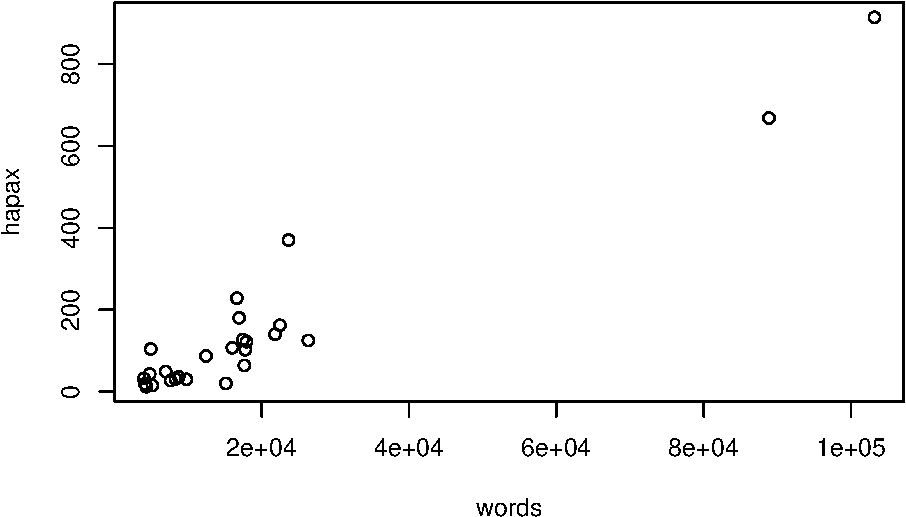
\includegraphics{_main_files/figure-latex/unnamed-chunk-35-1.pdf}

Это можно записать и иначе: \texttt{plot(hapax\_plato\$hapax\ \textasciitilde{}\ hapax\_plato\$words)}. Результат будет одинаковый.

Теперь беремся за палитру. Данные скучились в левом нижнем углу и потому плохо читаются. Мы можем пожертвовать двумя очень длинными диалогами (это ``Государство'' и ``Законы'') и ``приблизить'' картинку, указав вручную границы осей.

\begin{Shaded}
\begin{Highlighting}[]
\FunctionTok{attach}\NormalTok{(hapax\_plato) }
\FunctionTok{plot}\NormalTok{(hapax }\SpecialCharTok{\textasciitilde{}}\NormalTok{ words, }\AttributeTok{xlim =} \FunctionTok{c}\NormalTok{(}\DecValTok{0}\NormalTok{, }\DecValTok{30000}\NormalTok{), }\AttributeTok{ylim =} \FunctionTok{c}\NormalTok{(}\DecValTok{0}\NormalTok{, }\DecValTok{500}\NormalTok{))  }
\end{Highlighting}
\end{Shaded}

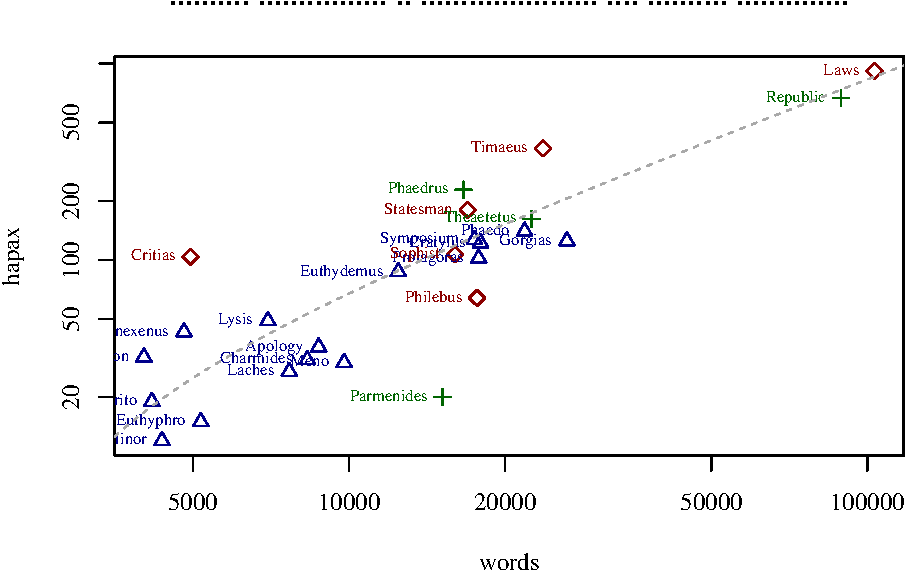
\includegraphics{_main_files/figure-latex/unnamed-chunk-36-1.pdf}

Но так мы все-таки теряем какую-то информацию -- а вдруг она важная? Еще один способ справиться со слипшимися данными -- преобразовать их. Применим логарифмическое преобразование. Обратите внимание, как меняются значения на осях.

\begin{Shaded}
\begin{Highlighting}[]
\FunctionTok{attach}\NormalTok{(hapax\_plato)}
\FunctionTok{options}\NormalTok{(}\AttributeTok{scipen=}\DecValTok{999}\NormalTok{) }\CommentTok{\# избавляет от научной нотации}
\FunctionTok{plot}\NormalTok{(words, hapax, }\AttributeTok{log =} \StringTok{"xy"}\NormalTok{)  }
\CommentTok{\# добавим текст}
\FunctionTok{text}\NormalTok{(hapax }\SpecialCharTok{\textasciitilde{}}\NormalTok{ words, }\AttributeTok{labels =}\NormalTok{ dialogue, }\AttributeTok{pos =} \DecValTok{2}\NormalTok{, }\AttributeTok{cex =} \FloatTok{0.7}\NormalTok{)}
\end{Highlighting}
\end{Shaded}

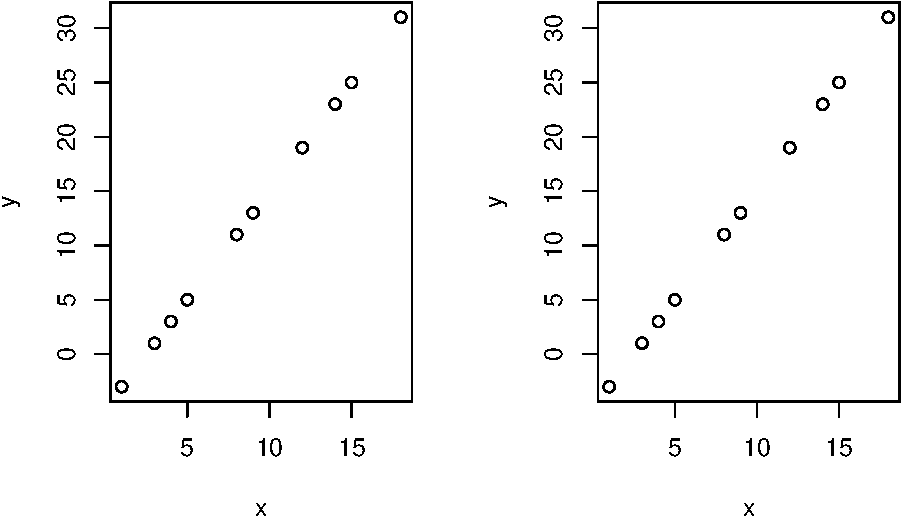
\includegraphics{_main_files/figure-latex/unnamed-chunk-37-1.pdf}

Уже гораздо интереснее! Попробуем обозначить цветом и формой пересказанные и прямые диалоги. Форма задается внутри функции \texttt{plot()} при помощи атрибута \texttt{pch}. Числовые значения этого атрибута соответствуют следующим значкам. Мы используем 2, 3 и 5.

\textbf{Добавить картинку: значения атрибута pch}

Перестраиваем наш график.

\begin{Shaded}
\begin{Highlighting}[]
\FunctionTok{attach}\NormalTok{(hapax\_plato)}
\FunctionTok{options}\NormalTok{(}\AttributeTok{scipen=}\DecValTok{999}\NormalTok{) }\CommentTok{\# избавляет от научной нотации}
\FunctionTok{plot}\NormalTok{(words, hapax, }\AttributeTok{log =} \StringTok{"xy"}\NormalTok{, }\AttributeTok{col =} \FunctionTok{c}\NormalTok{(}\StringTok{"darkblue"}\NormalTok{, }\StringTok{"darkgreen"}\NormalTok{, }\StringTok{"darkred"}\NormalTok{)[group], }
     \AttributeTok{pch =} \FunctionTok{c}\NormalTok{(}\DecValTok{2}\NormalTok{, }\DecValTok{3}\NormalTok{, }\DecValTok{5}\NormalTok{)[group])}
\FunctionTok{text}\NormalTok{(hapax }\SpecialCharTok{\textasciitilde{}}\NormalTok{ words, }\AttributeTok{labels =}\NormalTok{ dialogue, }
     \AttributeTok{pos =} \DecValTok{2}\NormalTok{, }\AttributeTok{cex =} \FloatTok{0.7}\NormalTok{, }\AttributeTok{col =} \FunctionTok{c}\NormalTok{(}\StringTok{"darkblue"}\NormalTok{, }\StringTok{"darkgreen"}\NormalTok{, }\StringTok{"darkred"}\NormalTok{)[group])}
\end{Highlighting}
\end{Shaded}

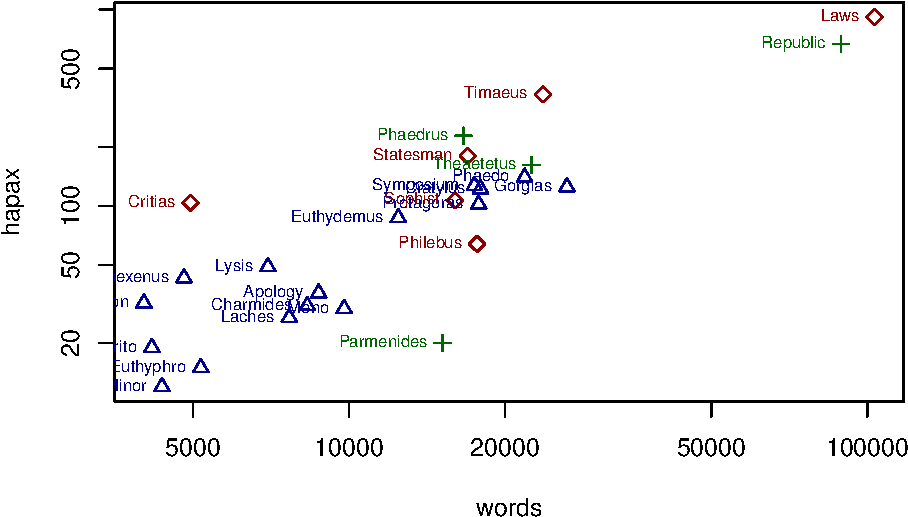
\includegraphics{_main_files/figure-latex/unnamed-chunk-38-1.pdf}

Некоторые названия перекрываютcя, но все равно намного понятнее. Теперь можем поменять шрифт и, например, добавить линию регрессии (не хватает легенды, но что-то уже нет сил).

\begin{Shaded}
\begin{Highlighting}[]
\FunctionTok{attach}\NormalTok{(hapax\_plato)}
\FunctionTok{options}\NormalTok{(}\AttributeTok{scipen=}\DecValTok{999}\NormalTok{) }\CommentTok{\# избавляет от научной нотации}
\FunctionTok{plot}\NormalTok{(words, hapax, }\AttributeTok{log =} \StringTok{"xy"}\NormalTok{, }\AttributeTok{col =} \FunctionTok{c}\NormalTok{(}\StringTok{"darkblue"}\NormalTok{, }\StringTok{"darkgreen"}\NormalTok{, }\StringTok{"darkred"}\NormalTok{)[group], }\AttributeTok{pch =} \FunctionTok{c}\NormalTok{(}\DecValTok{2}\NormalTok{, }\DecValTok{3}\NormalTok{, }\DecValTok{5}\NormalTok{)[group], }\AttributeTok{family =} \StringTok{"serif"}\NormalTok{)}
\FunctionTok{text}\NormalTok{(hapax }\SpecialCharTok{\textasciitilde{}}\NormalTok{ words, }\AttributeTok{labels =}\NormalTok{ dialogue, }
     \AttributeTok{pos =} \DecValTok{2}\NormalTok{, }\AttributeTok{cex =} \FloatTok{0.7}\NormalTok{, }\AttributeTok{col =} \FunctionTok{c}\NormalTok{(}\StringTok{"darkblue"}\NormalTok{, }\StringTok{"darkgreen"}\NormalTok{, }\StringTok{"darkred"}\NormalTok{)[group], }\AttributeTok{family =} \StringTok{"serif"}\NormalTok{)}

\CommentTok{\# добавим линию регрессии}
\NormalTok{my\_lm }\OtherTok{\textless{}{-}} \FunctionTok{lm}\NormalTok{(hapax\_plato}\SpecialCharTok{$}\NormalTok{hapax }\SpecialCharTok{\textasciitilde{}}\NormalTok{ hapax\_plato}\SpecialCharTok{$}\NormalTok{words)}
\FunctionTok{abline}\NormalTok{(my\_lm, }\AttributeTok{lty =} \StringTok{"dashed"}\NormalTok{, }\AttributeTok{col =} \StringTok{"darkgrey"}\NormalTok{, }\AttributeTok{untf =}\NormalTok{ T)}

\CommentTok{\# и заголовок}
\FunctionTok{title}\NormalTok{(}\AttributeTok{main =} \StringTok{"Число гапаксов в зависимости от длины диалога"}\NormalTok{)}
\end{Highlighting}
\end{Shaded}

\begin{verbatim}
## Warning in title(main = "Число гапаксов в зависимости от длины диалога"):
## conversion failure on 'Число гапаксов в зависимости от длины диалога' in
## 'mbcsToSbcs': dot substituted for <d0>
\end{verbatim}

\begin{verbatim}
## Warning in title(main = "Число гапаксов в зависимости от длины диалога"):
## conversion failure on 'Число гапаксов в зависимости от длины диалога' in
## 'mbcsToSbcs': dot substituted for <a7>
\end{verbatim}

\begin{verbatim}
## Warning in title(main = "Число гапаксов в зависимости от длины диалога"):
## conversion failure on 'Число гапаксов в зависимости от длины диалога' in
## 'mbcsToSbcs': dot substituted for <d0>
\end{verbatim}

\begin{verbatim}
## Warning in title(main = "Число гапаксов в зависимости от длины диалога"):
## conversion failure on 'Число гапаксов в зависимости от длины диалога' in
## 'mbcsToSbcs': dot substituted for <b8>
\end{verbatim}

\begin{verbatim}
## Warning in title(main = "Число гапаксов в зависимости от длины диалога"):
## conversion failure on 'Число гапаксов в зависимости от длины диалога' in
## 'mbcsToSbcs': dot substituted for <d1>
\end{verbatim}

\begin{verbatim}
## Warning in title(main = "Число гапаксов в зависимости от длины диалога"):
## conversion failure on 'Число гапаксов в зависимости от длины диалога' in
## 'mbcsToSbcs': dot substituted for <81>
\end{verbatim}

\begin{verbatim}
## Warning in title(main = "Число гапаксов в зависимости от длины диалога"):
## conversion failure on 'Число гапаксов в зависимости от длины диалога' in
## 'mbcsToSbcs': dot substituted for <d0>
\end{verbatim}

\begin{verbatim}
## Warning in title(main = "Число гапаксов в зависимости от длины диалога"):
## conversion failure on 'Число гапаксов в зависимости от длины диалога' in
## 'mbcsToSbcs': dot substituted for <bb>
\end{verbatim}

\begin{verbatim}
## Warning in title(main = "Число гапаксов в зависимости от длины диалога"):
## conversion failure on 'Число гапаксов в зависимости от длины диалога' in
## 'mbcsToSbcs': dot substituted for <d0>
\end{verbatim}

\begin{verbatim}
## Warning in title(main = "Число гапаксов в зависимости от длины диалога"):
## conversion failure on 'Число гапаксов в зависимости от длины диалога' in
## 'mbcsToSbcs': dot substituted for <be>
\end{verbatim}

\begin{verbatim}
## Warning in title(main = "Число гапаксов в зависимости от длины диалога"):
## conversion failure on 'Число гапаксов в зависимости от длины диалога' in
## 'mbcsToSbcs': dot substituted for <d0>
\end{verbatim}

\begin{verbatim}
## Warning in title(main = "Число гапаксов в зависимости от длины диалога"):
## conversion failure on 'Число гапаксов в зависимости от длины диалога' in
## 'mbcsToSbcs': dot substituted for <b3>
\end{verbatim}

\begin{verbatim}
## Warning in title(main = "Число гапаксов в зависимости от длины диалога"):
## conversion failure on 'Число гапаксов в зависимости от длины диалога' in
## 'mbcsToSbcs': dot substituted for <d0>
\end{verbatim}

\begin{verbatim}
## Warning in title(main = "Число гапаксов в зависимости от длины диалога"):
## conversion failure on 'Число гапаксов в зависимости от длины диалога' in
## 'mbcsToSbcs': dot substituted for <b0>
\end{verbatim}

\begin{verbatim}
## Warning in title(main = "Число гапаксов в зависимости от длины диалога"):
## conversion failure on 'Число гапаксов в зависимости от длины диалога' in
## 'mbcsToSbcs': dot substituted for <d0>
\end{verbatim}

\begin{verbatim}
## Warning in title(main = "Число гапаксов в зависимости от длины диалога"):
## conversion failure on 'Число гапаксов в зависимости от длины диалога' in
## 'mbcsToSbcs': dot substituted for <bf>
\end{verbatim}

\begin{verbatim}
## Warning in title(main = "Число гапаксов в зависимости от длины диалога"):
## conversion failure on 'Число гапаксов в зависимости от длины диалога' in
## 'mbcsToSbcs': dot substituted for <d0>
\end{verbatim}

\begin{verbatim}
## Warning in title(main = "Число гапаксов в зависимости от длины диалога"):
## conversion failure on 'Число гапаксов в зависимости от длины диалога' in
## 'mbcsToSbcs': dot substituted for <b0>
\end{verbatim}

\begin{verbatim}
## Warning in title(main = "Число гапаксов в зависимости от длины диалога"):
## conversion failure on 'Число гапаксов в зависимости от длины диалога' in
## 'mbcsToSbcs': dot substituted for <d0>
\end{verbatim}

\begin{verbatim}
## Warning in title(main = "Число гапаксов в зависимости от длины диалога"):
## conversion failure on 'Число гапаксов в зависимости от длины диалога' in
## 'mbcsToSbcs': dot substituted for <ba>
\end{verbatim}

\begin{verbatim}
## Warning in title(main = "Число гапаксов в зависимости от длины диалога"):
## conversion failure on 'Число гапаксов в зависимости от длины диалога' in
## 'mbcsToSbcs': dot substituted for <d1>
\end{verbatim}

\begin{verbatim}
## Warning in title(main = "Число гапаксов в зависимости от длины диалога"):
## conversion failure on 'Число гапаксов в зависимости от длины диалога' in
## 'mbcsToSbcs': dot substituted for <81>
\end{verbatim}

\begin{verbatim}
## Warning in title(main = "Число гапаксов в зависимости от длины диалога"):
## conversion failure on 'Число гапаксов в зависимости от длины диалога' in
## 'mbcsToSbcs': dot substituted for <d0>
\end{verbatim}

\begin{verbatim}
## Warning in title(main = "Число гапаксов в зависимости от длины диалога"):
## conversion failure on 'Число гапаксов в зависимости от длины диалога' in
## 'mbcsToSbcs': dot substituted for <be>
\end{verbatim}

\begin{verbatim}
## Warning in title(main = "Число гапаксов в зависимости от длины диалога"):
## conversion failure on 'Число гапаксов в зависимости от длины диалога' in
## 'mbcsToSbcs': dot substituted for <d0>
\end{verbatim}

\begin{verbatim}
## Warning in title(main = "Число гапаксов в зависимости от длины диалога"):
## conversion failure on 'Число гапаксов в зависимости от длины диалога' in
## 'mbcsToSbcs': dot substituted for <b2>
\end{verbatim}

\begin{verbatim}
## Warning in title(main = "Число гапаксов в зависимости от длины диалога"):
## conversion failure on 'Число гапаксов в зависимости от длины диалога' in
## 'mbcsToSbcs': dot substituted for <d0>
\end{verbatim}

\begin{verbatim}
## Warning in title(main = "Число гапаксов в зависимости от длины диалога"):
## conversion failure on 'Число гапаксов в зависимости от длины диалога' in
## 'mbcsToSbcs': dot substituted for <b2>
\end{verbatim}

\begin{verbatim}
## Warning in title(main = "Число гапаксов в зависимости от длины диалога"):
## conversion failure on 'Число гапаксов в зависимости от длины диалога' in
## 'mbcsToSbcs': dot substituted for <d0>
\end{verbatim}

\begin{verbatim}
## Warning in title(main = "Число гапаксов в зависимости от длины диалога"):
## conversion failure on 'Число гапаксов в зависимости от длины диалога' in
## 'mbcsToSbcs': dot substituted for <b7>
\end{verbatim}

\begin{verbatim}
## Warning in title(main = "Число гапаксов в зависимости от длины диалога"):
## conversion failure on 'Число гапаксов в зависимости от длины диалога' in
## 'mbcsToSbcs': dot substituted for <d0>
\end{verbatim}

\begin{verbatim}
## Warning in title(main = "Число гапаксов в зависимости от длины диалога"):
## conversion failure on 'Число гапаксов в зависимости от длины диалога' in
## 'mbcsToSbcs': dot substituted for <b0>
\end{verbatim}

\begin{verbatim}
## Warning in title(main = "Число гапаксов в зависимости от длины диалога"):
## conversion failure on 'Число гапаксов в зависимости от длины диалога' in
## 'mbcsToSbcs': dot substituted for <d0>
\end{verbatim}

\begin{verbatim}
## Warning in title(main = "Число гапаксов в зависимости от длины диалога"):
## conversion failure on 'Число гапаксов в зависимости от длины диалога' in
## 'mbcsToSbcs': dot substituted for <b2>
\end{verbatim}

\begin{verbatim}
## Warning in title(main = "Число гапаксов в зависимости от длины диалога"):
## conversion failure on 'Число гапаксов в зависимости от длины диалога' in
## 'mbcsToSbcs': dot substituted for <d0>
\end{verbatim}

\begin{verbatim}
## Warning in title(main = "Число гапаксов в зависимости от длины диалога"):
## conversion failure on 'Число гапаксов в зависимости от длины диалога' in
## 'mbcsToSbcs': dot substituted for <b8>
\end{verbatim}

\begin{verbatim}
## Warning in title(main = "Число гапаксов в зависимости от длины диалога"):
## conversion failure on 'Число гапаксов в зависимости от длины диалога' in
## 'mbcsToSbcs': dot substituted for <d1>
\end{verbatim}

\begin{verbatim}
## Warning in title(main = "Число гапаксов в зависимости от длины диалога"):
## conversion failure on 'Число гапаксов в зависимости от длины диалога' in
## 'mbcsToSbcs': dot substituted for <81>
\end{verbatim}

\begin{verbatim}
## Warning in title(main = "Число гапаксов в зависимости от длины диалога"):
## conversion failure on 'Число гапаксов в зависимости от длины диалога' in
## 'mbcsToSbcs': dot substituted for <d0>
\end{verbatim}

\begin{verbatim}
## Warning in title(main = "Число гапаксов в зависимости от длины диалога"):
## conversion failure on 'Число гапаксов в зависимости от длины диалога' in
## 'mbcsToSbcs': dot substituted for <b8>
\end{verbatim}

\begin{verbatim}
## Warning in title(main = "Число гапаксов в зависимости от длины диалога"):
## conversion failure on 'Число гапаксов в зависимости от длины диалога' in
## 'mbcsToSbcs': dot substituted for <d0>
\end{verbatim}

\begin{verbatim}
## Warning in title(main = "Число гапаксов в зависимости от длины диалога"):
## conversion failure on 'Число гапаксов в зависимости от длины диалога' in
## 'mbcsToSbcs': dot substituted for <bc>
\end{verbatim}

\begin{verbatim}
## Warning in title(main = "Число гапаксов в зависимости от длины диалога"):
## conversion failure on 'Число гапаксов в зависимости от длины диалога' in
## 'mbcsToSbcs': dot substituted for <d0>
\end{verbatim}

\begin{verbatim}
## Warning in title(main = "Число гапаксов в зависимости от длины диалога"):
## conversion failure on 'Число гапаксов в зависимости от длины диалога' in
## 'mbcsToSbcs': dot substituted for <be>
\end{verbatim}

\begin{verbatim}
## Warning in title(main = "Число гапаксов в зависимости от длины диалога"):
## conversion failure on 'Число гапаксов в зависимости от длины диалога' in
## 'mbcsToSbcs': dot substituted for <d1>
\end{verbatim}

\begin{verbatim}
## Warning in title(main = "Число гапаксов в зависимости от длины диалога"):
## conversion failure on 'Число гапаксов в зависимости от длины диалога' in
## 'mbcsToSbcs': dot substituted for <81>
\end{verbatim}

\begin{verbatim}
## Warning in title(main = "Число гапаксов в зависимости от длины диалога"):
## conversion failure on 'Число гапаксов в зависимости от длины диалога' in
## 'mbcsToSbcs': dot substituted for <d1>
\end{verbatim}

\begin{verbatim}
## Warning in title(main = "Число гапаксов в зависимости от длины диалога"):
## conversion failure on 'Число гапаксов в зависимости от длины диалога' in
## 'mbcsToSbcs': dot substituted for <82>
\end{verbatim}

\begin{verbatim}
## Warning in title(main = "Число гапаксов в зависимости от длины диалога"):
## conversion failure on 'Число гапаксов в зависимости от длины диалога' in
## 'mbcsToSbcs': dot substituted for <d0>
\end{verbatim}

\begin{verbatim}
## Warning in title(main = "Число гапаксов в зависимости от длины диалога"):
## conversion failure on 'Число гапаксов в зависимости от длины диалога' in
## 'mbcsToSbcs': dot substituted for <b8>
\end{verbatim}

\begin{verbatim}
## Warning in title(main = "Число гапаксов в зависимости от длины диалога"):
## conversion failure on 'Число гапаксов в зависимости от длины диалога' in
## 'mbcsToSbcs': dot substituted for <d0>
\end{verbatim}

\begin{verbatim}
## Warning in title(main = "Число гапаксов в зависимости от длины диалога"):
## conversion failure on 'Число гапаксов в зависимости от длины диалога' in
## 'mbcsToSbcs': dot substituted for <be>
\end{verbatim}

\begin{verbatim}
## Warning in title(main = "Число гапаксов в зависимости от длины диалога"):
## conversion failure on 'Число гапаксов в зависимости от длины диалога' in
## 'mbcsToSbcs': dot substituted for <d1>
\end{verbatim}

\begin{verbatim}
## Warning in title(main = "Число гапаксов в зависимости от длины диалога"):
## conversion failure on 'Число гапаксов в зависимости от длины диалога' in
## 'mbcsToSbcs': dot substituted for <82>
\end{verbatim}

\begin{verbatim}
## Warning in title(main = "Число гапаксов в зависимости от длины диалога"):
## conversion failure on 'Число гапаксов в зависимости от длины диалога' in
## 'mbcsToSbcs': dot substituted for <d0>
\end{verbatim}

\begin{verbatim}
## Warning in title(main = "Число гапаксов в зависимости от длины диалога"):
## conversion failure on 'Число гапаксов в зависимости от длины диалога' in
## 'mbcsToSbcs': dot substituted for <b4>
\end{verbatim}

\begin{verbatim}
## Warning in title(main = "Число гапаксов в зависимости от длины диалога"):
## conversion failure on 'Число гапаксов в зависимости от длины диалога' in
## 'mbcsToSbcs': dot substituted for <d0>
\end{verbatim}

\begin{verbatim}
## Warning in title(main = "Число гапаксов в зависимости от длины диалога"):
## conversion failure on 'Число гапаксов в зависимости от длины диалога' in
## 'mbcsToSbcs': dot substituted for <bb>
\end{verbatim}

\begin{verbatim}
## Warning in title(main = "Число гапаксов в зависимости от длины диалога"):
## conversion failure on 'Число гапаксов в зависимости от длины диалога' in
## 'mbcsToSbcs': dot substituted for <d0>
\end{verbatim}

\begin{verbatim}
## Warning in title(main = "Число гапаксов в зависимости от длины диалога"):
## conversion failure on 'Число гапаксов в зависимости от длины диалога' in
## 'mbcsToSbcs': dot substituted for <b8>
\end{verbatim}

\begin{verbatim}
## Warning in title(main = "Число гапаксов в зависимости от длины диалога"):
## conversion failure on 'Число гапаксов в зависимости от длины диалога' in
## 'mbcsToSbcs': dot substituted for <d0>
\end{verbatim}

\begin{verbatim}
## Warning in title(main = "Число гапаксов в зависимости от длины диалога"):
## conversion failure on 'Число гапаксов в зависимости от длины диалога' in
## 'mbcsToSbcs': dot substituted for <bd>
\end{verbatim}

\begin{verbatim}
## Warning in title(main = "Число гапаксов в зависимости от длины диалога"):
## conversion failure on 'Число гапаксов в зависимости от длины диалога' in
## 'mbcsToSbcs': dot substituted for <d1>
\end{verbatim}

\begin{verbatim}
## Warning in title(main = "Число гапаксов в зависимости от длины диалога"):
## conversion failure on 'Число гапаксов в зависимости от длины диалога' in
## 'mbcsToSbcs': dot substituted for <8b>
\end{verbatim}

\begin{verbatim}
## Warning in title(main = "Число гапаксов в зависимости от длины диалога"):
## conversion failure on 'Число гапаксов в зависимости от длины диалога' in
## 'mbcsToSbcs': dot substituted for <d0>
\end{verbatim}

\begin{verbatim}
## Warning in title(main = "Число гапаксов в зависимости от длины диалога"):
## conversion failure on 'Число гапаксов в зависимости от длины диалога' in
## 'mbcsToSbcs': dot substituted for <b4>
\end{verbatim}

\begin{verbatim}
## Warning in title(main = "Число гапаксов в зависимости от длины диалога"):
## conversion failure on 'Число гапаксов в зависимости от длины диалога' in
## 'mbcsToSbcs': dot substituted for <d0>
\end{verbatim}

\begin{verbatim}
## Warning in title(main = "Число гапаксов в зависимости от длины диалога"):
## conversion failure on 'Число гапаксов в зависимости от длины диалога' in
## 'mbcsToSbcs': dot substituted for <b8>
\end{verbatim}

\begin{verbatim}
## Warning in title(main = "Число гапаксов в зависимости от длины диалога"):
## conversion failure on 'Число гапаксов в зависимости от длины диалога' in
## 'mbcsToSbcs': dot substituted for <d0>
\end{verbatim}

\begin{verbatim}
## Warning in title(main = "Число гапаксов в зависимости от длины диалога"):
## conversion failure on 'Число гапаксов в зависимости от длины диалога' in
## 'mbcsToSbcs': dot substituted for <b0>
\end{verbatim}

\begin{verbatim}
## Warning in title(main = "Число гапаксов в зависимости от длины диалога"):
## conversion failure on 'Число гапаксов в зависимости от длины диалога' in
## 'mbcsToSbcs': dot substituted for <d0>
\end{verbatim}

\begin{verbatim}
## Warning in title(main = "Число гапаксов в зависимости от длины диалога"):
## conversion failure on 'Число гапаксов в зависимости от длины диалога' in
## 'mbcsToSbcs': dot substituted for <bb>
\end{verbatim}

\begin{verbatim}
## Warning in title(main = "Число гапаксов в зависимости от длины диалога"):
## conversion failure on 'Число гапаксов в зависимости от длины диалога' in
## 'mbcsToSbcs': dot substituted for <d0>
\end{verbatim}

\begin{verbatim}
## Warning in title(main = "Число гапаксов в зависимости от длины диалога"):
## conversion failure on 'Число гапаксов в зависимости от длины диалога' in
## 'mbcsToSbcs': dot substituted for <be>
\end{verbatim}

\begin{verbatim}
## Warning in title(main = "Число гапаксов в зависимости от длины диалога"):
## conversion failure on 'Число гапаксов в зависимости от длины диалога' in
## 'mbcsToSbcs': dot substituted for <d0>
\end{verbatim}

\begin{verbatim}
## Warning in title(main = "Число гапаксов в зависимости от длины диалога"):
## conversion failure on 'Число гапаксов в зависимости от длины диалога' in
## 'mbcsToSbcs': dot substituted for <b3>
\end{verbatim}

\begin{verbatim}
## Warning in title(main = "Число гапаксов в зависимости от длины диалога"):
## conversion failure on 'Число гапаксов в зависимости от длины диалога' in
## 'mbcsToSbcs': dot substituted for <d0>
\end{verbatim}

\begin{verbatim}
## Warning in title(main = "Число гапаксов в зависимости от длины диалога"):
## conversion failure on 'Число гапаксов в зависимости от длины диалога' in
## 'mbcsToSbcs': dot substituted for <b0>
\end{verbatim}

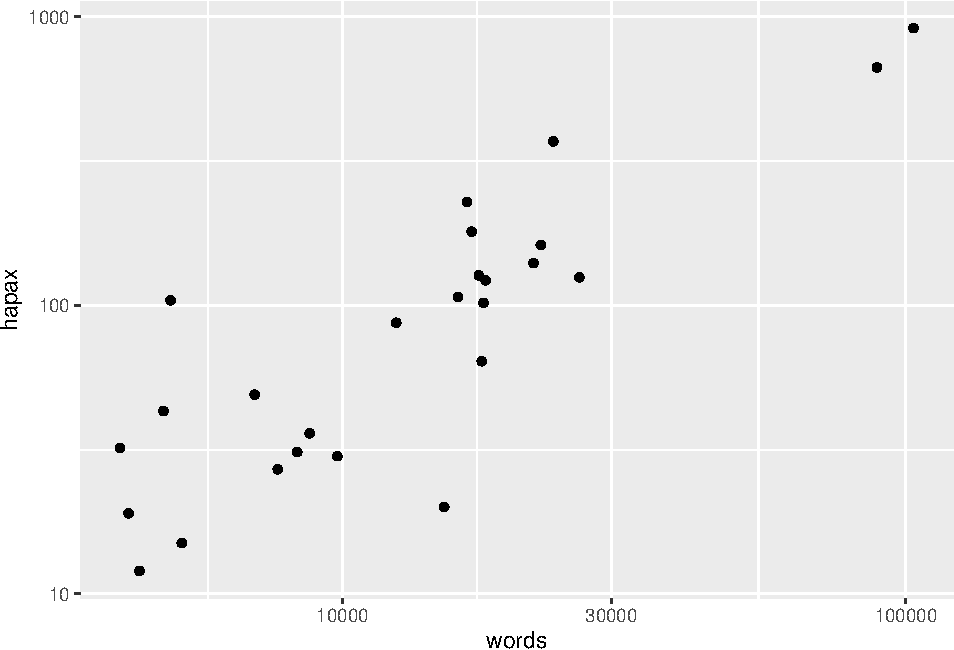
\includegraphics{_main_files/figure-latex/unnamed-chunk-39-1.pdf}

При помощи \textbf{графических параметров}\footnote{\url{https://www.rdocumentation.org/packages/graphics/versions/3.6.2/topics/par}} можно контролировать множество настроек. Но в этом и недостаток базовой графики. Не всем хватает терпения и вкуса этим заниматься, поэтому эта система сейчас не очень употребительна.

Мы построили только диаграмму рассеяния, но в базовом R можно делать и гистограммы, и диаграмму размаха, и другие графики.

Попробуйте интерпретировать график, который у нас получился. Прав ли был профессор Кэмпбелл, утверждая, что высокая доля гапаксов характерна для ``поздних'' текстов? Исходите из того, что ни для одного текста мы не знаем дату написания.

{\emph{Судя по графику, количество гапаксов зависит от количества слов в тексте. Чем длиннее текст, тем больше вероятность встретить там редкое слово.}}

\hypertarget{lattice}{%
\section{Lattice}\label{lattice}}

Система Lattice (букв. ``Решетка'') была разработана специально для анализа многомерных данных \citep{sarkar2008}.

\textbf{Тут должны быть \st{графики} цветочки}

Например, мы сравниваем точность классификации текстов в зависимости от длины отрывка и количества слов-предикторов. Это уже три переменные (длина -- количество слов -- точность). Система решеток, или панелей, позволяет представить такие многомерные данные. \textbf{Добавить ссылку}

В базовом R это тоже можно сделать, изменив графические параметры:

\begin{Shaded}
\begin{Highlighting}[]
\NormalTok{x }\OtherTok{\textless{}{-}} \FunctionTok{sample}\NormalTok{(}\DecValTok{1}\SpecialCharTok{:}\DecValTok{20}\NormalTok{, }\DecValTok{10}\NormalTok{)}
\NormalTok{y }\OtherTok{\textless{}{-}} \DecValTok{2} \SpecialCharTok{*}\NormalTok{ x  }\SpecialCharTok{{-}} \DecValTok{5}
\FunctionTok{par}\NormalTok{(}\AttributeTok{mfrow =} \FunctionTok{c}\NormalTok{(}\DecValTok{1}\NormalTok{,}\DecValTok{2}\NormalTok{)) }\CommentTok{\# вот тут указываем число рядов и столбцов}
\FunctionTok{plot}\NormalTok{(x, y)}
\FunctionTok{plot}\NormalTok{(x, y)}
\end{Highlighting}
\end{Shaded}

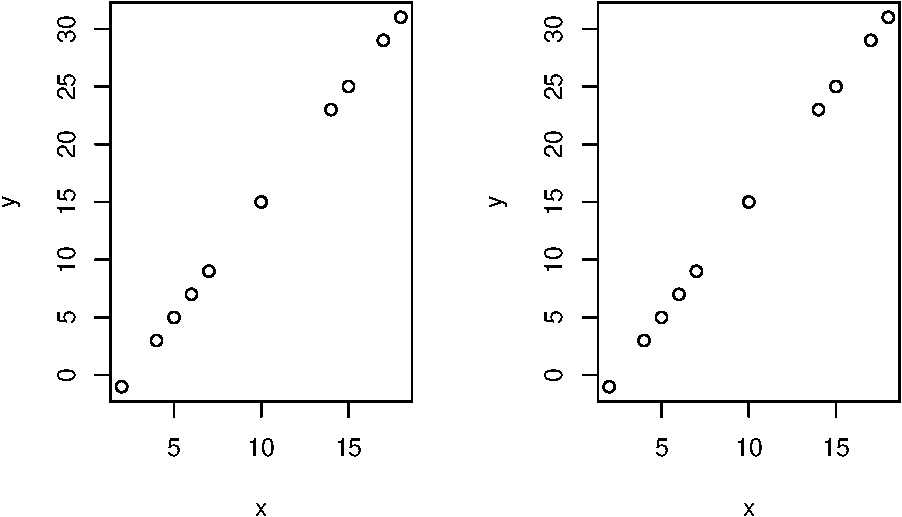
\includegraphics{_main_files/figure-latex/unnamed-chunk-40-1.pdf}

Но видно, что пространство при этом расходуется неэффективно. Кроме того, к таким графикам сложно создавать заголовки и подзаголовки, подбирать подписи и т.п. Все эти задачи решает Lattice.

Идея этой системы в том, что каждый график строится с помощью одного вызова функции. При этом необходимо сразу указать большое количество информации, чтобы у фунцкии было достаточно данных для построения графика.

\begin{Shaded}
\begin{Highlighting}[]
\FunctionTok{library}\NormalTok{(lattice)}
\FunctionTok{attach}\NormalTok{(hapax\_plato)}

\CommentTok{\# после вертикальной черты указана переменная, которая используется для группировки данных; в нашем случае номер группы (по Кэмпбеллу)}

\FunctionTok{xyplot}\NormalTok{(hapax }\SpecialCharTok{\textasciitilde{}}\NormalTok{ words }\SpecialCharTok{|}\NormalTok{ group, }\AttributeTok{data =}\NormalTok{ hapax\_plato,}
       \AttributeTok{scales=}\FunctionTok{list}\NormalTok{(}\AttributeTok{x=}\FunctionTok{list}\NormalTok{(}\AttributeTok{log=}\DecValTok{10}\NormalTok{))) }\CommentTok{\# трансформация по одной оси}
\end{Highlighting}
\end{Shaded}

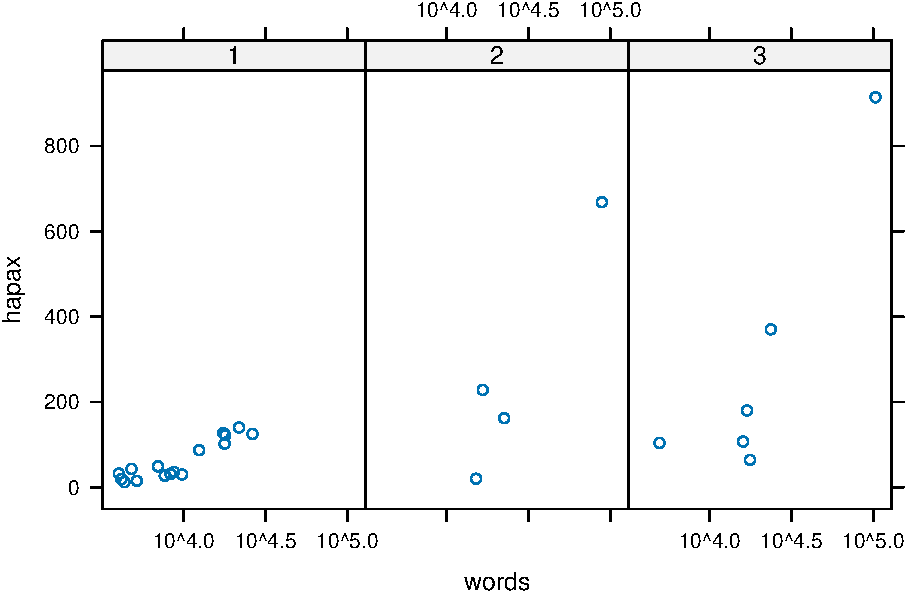
\includegraphics{_main_files/figure-latex/unnamed-chunk-41-1.pdf}

Недостаток Lattice, однако, в том, что бывает сложно аннотировать отдельные панели, а также приходится сразу задавать весь график в одном вызове функции. Это не всегда удобно. После создания графика уже ничего нельзя добавить или убавить.

\hypertarget{ggplot2}{%
\section{Ggplot2}\label{ggplot2}}

Но настоящая графическая сила R -- это пакет ggplot2. В его основе лежит идея ``грамматики графических элементов'' Лиланда Уилкинсона \citep{мастицкий2017}, и он позволяет объединить достоинства базовой графики R и Lattice. С одной стороны, вы можете постепенно достраивать график, добавляя элемент за элементом; с другой стороны, множество параметров подбираются автоматически, как в Lattice.

\hypertarget{ux431ux44bux441ux442ux440ux43eux435-ux440ux435ux448ux435ux43dux438ux435-qplot}{%
\subsection{Быстрое решение: qplot()}\label{ux431ux44bux441ux442ux440ux43eux435-ux440ux435ux448ux435ux43dux438ux435-qplot}}

Настройки по умолчанию хорошо видно на графике ниже; их легко перенастроить.

\begin{Shaded}
\begin{Highlighting}[]
\FunctionTok{library}\NormalTok{(ggplot2) }\CommentTok{\# загружается сразу с tidyverse}
\FunctionTok{options}\NormalTok{(}\AttributeTok{scipen =} \DecValTok{999}\NormalTok{)}
\FunctionTok{qplot}\NormalTok{(words, hapax, }\AttributeTok{data =}\NormalTok{ hapax\_plato, }\AttributeTok{log =} \StringTok{"xy"}\NormalTok{)}
\end{Highlighting}
\end{Shaded}

\begin{verbatim}
## Warning: `qplot()` was deprecated in ggplot2 3.4.0.
## This warning is displayed once every 8 hours.
## Call `lifecycle::last_lifecycle_warnings()` to see where this warning was
## generated.
\end{verbatim}

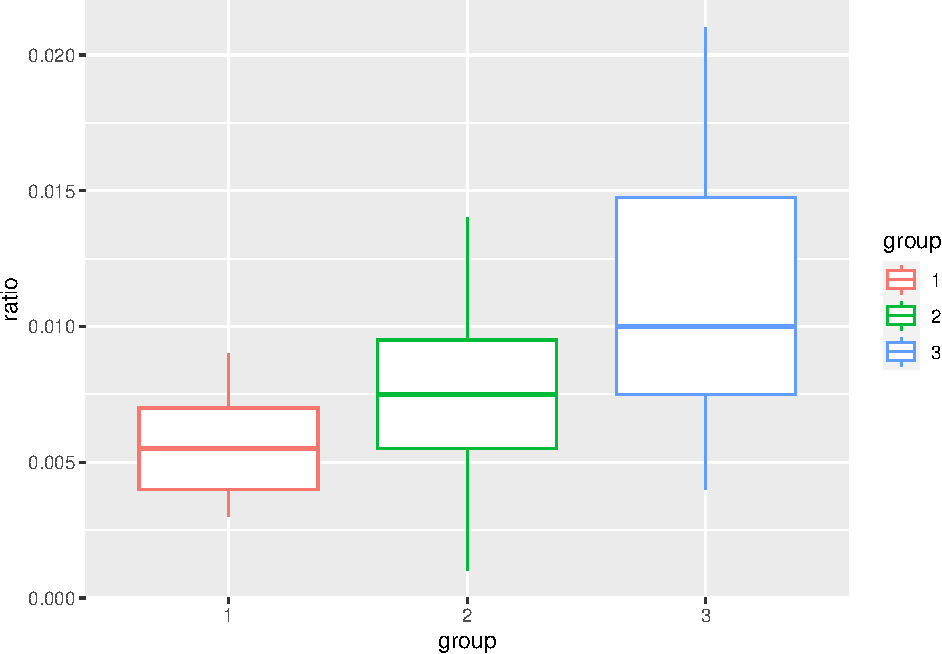
\includegraphics{_main_files/figure-latex/unnamed-chunk-42-1.pdf}

Функция \texttt{qplot()} -- это быстрое решение для задач визуализации.

В современных версиях ggplot использование функции \texttt{qplot()} не рекомендуется (deprecated), чтобы побудить пользователей изучать \texttt{ggplot()} как более совершенный инструмент для визуализаций.

В данном случае мы построили диаграмму рассеяния, используя логарифмическую трансформацию по двум осям. Можно также выделить цветом различные типы диалогов, изменить размер точек, их прозначность и т.п.

\begin{Shaded}
\begin{Highlighting}[]
\FunctionTok{qplot}\NormalTok{(words, hapax, }\AttributeTok{data =}\NormalTok{ hapax\_plato, }\AttributeTok{log =} \StringTok{"xy"}\NormalTok{, }\AttributeTok{col =}\NormalTok{ group, }\AttributeTok{size =} \FloatTok{1.5}\NormalTok{) }\SpecialCharTok{+} \FunctionTok{theme}\NormalTok{(}\AttributeTok{legend.position =} \StringTok{"none"}\NormalTok{)}
\end{Highlighting}
\end{Shaded}

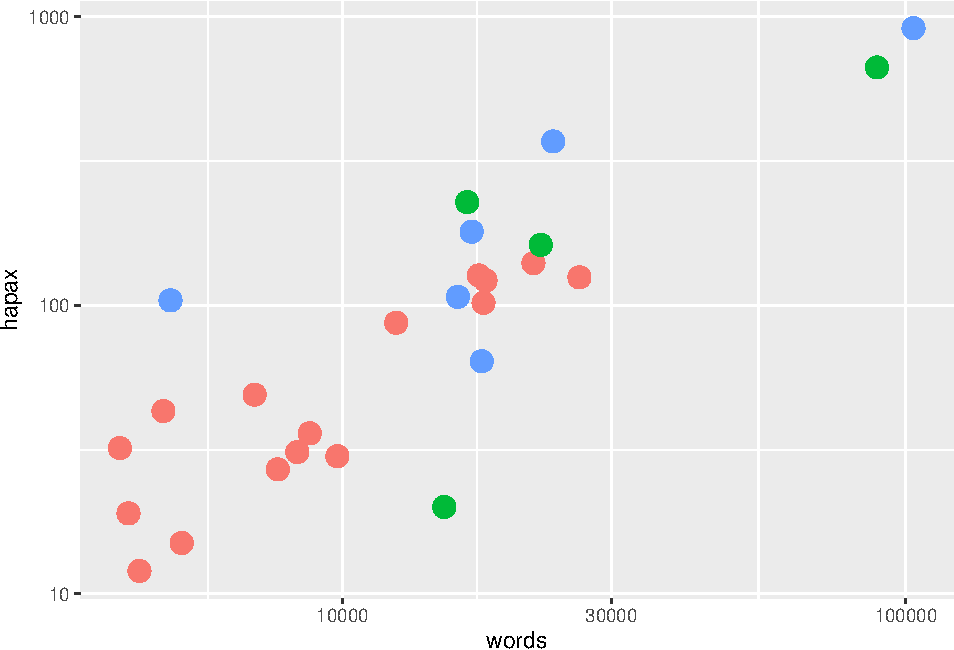
\includegraphics{_main_files/figure-latex/unnamed-chunk-43-1.pdf}

\textbf{Линия тренда} (сглаживающая линия) добавляется следующим образом:

\begin{Shaded}
\begin{Highlighting}[]
\FunctionTok{qplot}\NormalTok{(words, hapax, }\AttributeTok{data =}\NormalTok{ hapax\_plato, }\AttributeTok{log =} \StringTok{"xy"}\NormalTok{, }\AttributeTok{geom =} \FunctionTok{c}\NormalTok{(}\StringTok{"point"}\NormalTok{, }\StringTok{"smooth"}\NormalTok{))}
\end{Highlighting}
\end{Shaded}

\begin{verbatim}
## `geom_smooth()` using method = 'loess' and formula = 'y ~ x'
\end{verbatim}

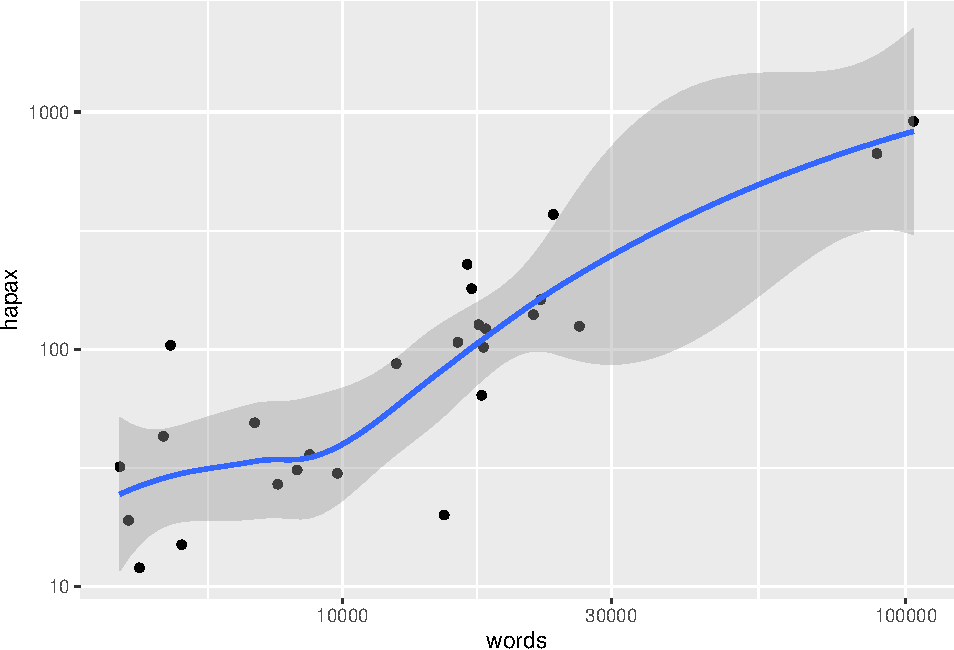
\includegraphics{_main_files/figure-latex/unnamed-chunk-44-1.pdf}

\textbf{Диаграмма размаха} (о ней подробнее можно посмотреть \href{https://vk.com/video_ext.php?oid=-211800158\&id=456239229\&hash=7e1bc800e53df22c\&hd=2}{здесь}) удобна в тех случаях, когда необходимо представить обобщенную статиситческую информацию о распределении значений количественной переменной в разных группах.

\begin{Shaded}
\begin{Highlighting}[]
\FunctionTok{attach}\NormalTok{(hapax\_plato)}
\FunctionTok{qplot}\NormalTok{(group, ratio, }\AttributeTok{data =}\NormalTok{ hapax\_plato, }\AttributeTok{geom =} \StringTok{"boxplot"}\NormalTok{, }\AttributeTok{color =}\NormalTok{ group)}
\end{Highlighting}
\end{Shaded}

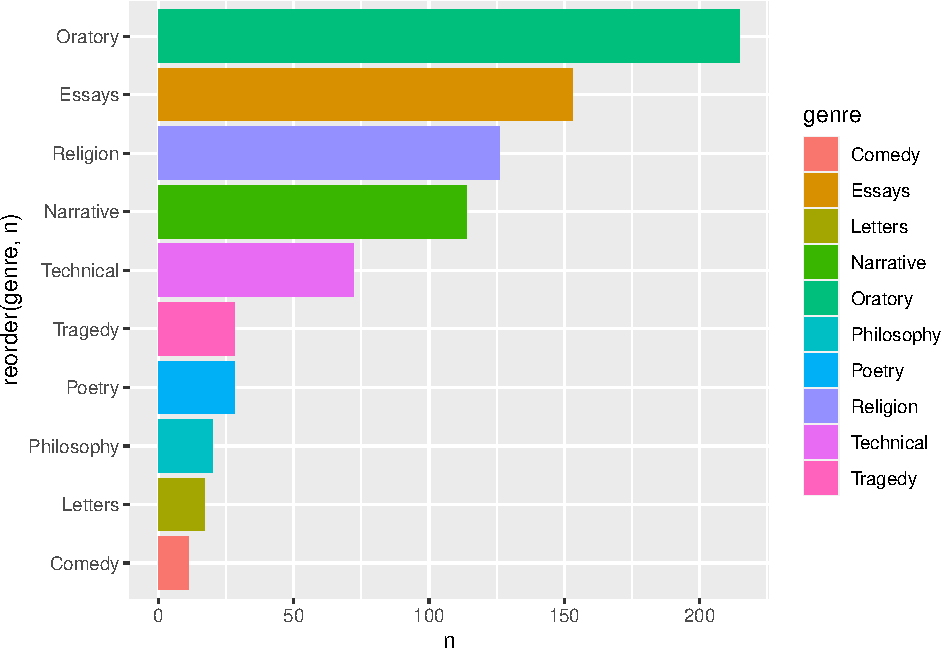
\includegraphics{_main_files/figure-latex/unnamed-chunk-45-1.pdf}

Диаграмму размаха можно совместить с \textbf{одномерной диаграммой рассеяния}.

\begin{Shaded}
\begin{Highlighting}[]
\FunctionTok{qplot}\NormalTok{(group, ratio, }\AttributeTok{data =}\NormalTok{ hapax\_plato, }\AttributeTok{geom =} \FunctionTok{c}\NormalTok{(}\StringTok{"boxplot"}\NormalTok{, }\StringTok{"jitter"}\NormalTok{), }\AttributeTok{color =}\NormalTok{ group) }\CommentTok{\# вместо color можно использовать shape, который отвечает за форму элементов}
\end{Highlighting}
\end{Shaded}

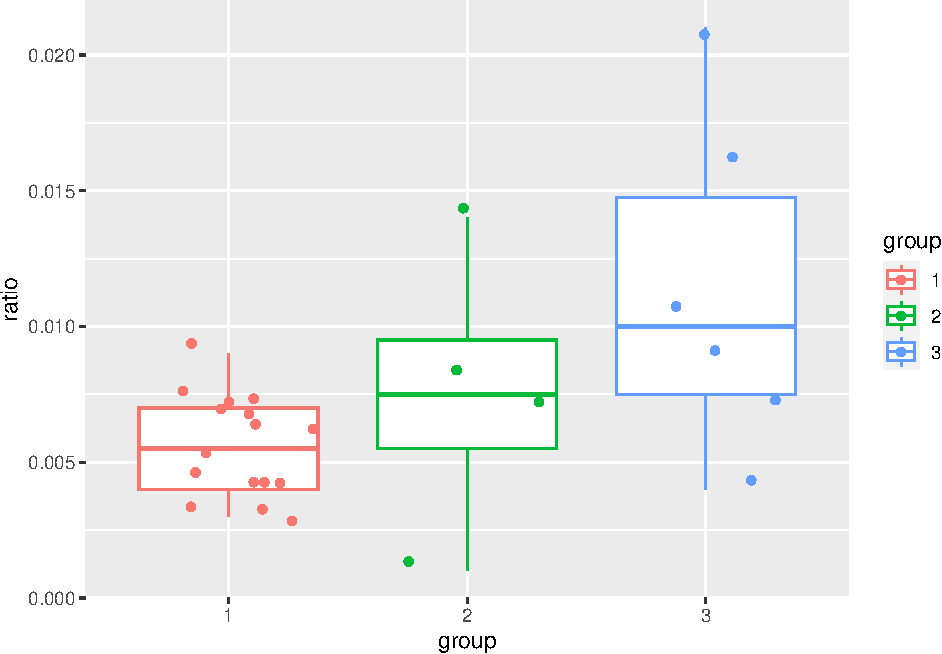
\includegraphics{_main_files/figure-latex/unnamed-chunk-46-1.pdf}

\hypertarget{ux441ux43bux43eux439-ux437ux430-ux441ux43bux43eux435ux43c-ggplot}{%
\subsection{Слой за слоем: ggplot()}\label{ux441ux43bux43eux439-ux437ux430-ux441ux43bux43eux435ux43c-ggplot}}

Для более детальной настройки графика рекомендууется использовать функцию \texttt{ggplot()}, которая имеет два основных аргумента: \texttt{data} и \texttt{aes} (англ. \emph{aesthetics}); последняя присваивает эстетические атрибуты геометрическим объектам, которые используются на графике. Эти объекты могут слоями накладываться друг на друга \citep{wickham2016}.

Посмотрим, как это работает, на примере, \textbf{столбиковой диаграммы}. Такая позволяет представить распределение как количественных, так и качественных переменных. Для примера возьмем датасет \texttt{diorisis\_meta}, который хранит данные о древнегреческих текстах, доступных в репозитории Diorisis\footnote{\url{https://figshare.com/articles/dataset/The_Diorisis_Ancient_Greek_Corpus/6187256}}.

\begin{Shaded}
\begin{Highlighting}[]
\FunctionTok{load}\NormalTok{(}\StringTok{"./datasets/DiorisisMeta.Rdata"}\NormalTok{)}
\NormalTok{diorisis\_meta}
\end{Highlighting}
\end{Shaded}

\begin{verbatim}
## # A tibble: 784 x 5
##    name            title                      date genre     subgenre       
##    <chr>           <chr>                     <dbl> <chr>     <chr>          
##  1 Achilles Tatius Leucippe and Clitophon      120 Narrative Novel          
##  2 Aelian          De Natura Animalium         230 Technical Natural History
##  3 Aelian          Epistulae Rusticae          230 Letters   Letters        
##  4 Aelian          Varia Historia              200 Essays    Miscellanea    
##  5 Aeneas Tacticus Poliorcetica               -350 Technical Military       
##  6 Aeschines       Against Ctesiphon          -330 Oratory   Oratory        
##  7 Aeschines       Against Timarchus          -347 Oratory   Oratory        
##  8 Aeschines       The Speech on the Embassy  -336 Oratory   Oratory        
##  9 Aeschylus       Agamemnon                  -458 Tragedy   Tragedy        
## 10 Aeschylus       Eumenides                  -458 Tragedy   Tragedy        
## # i 774 more rows
\end{verbatim}

Столбиковая диаграмма позволяет увидеть, тексты каких жанров чаще всего встречаются в этом корпусе.

\begin{Shaded}
\begin{Highlighting}[]
\FunctionTok{library}\NormalTok{(tidyverse)}
\NormalTok{diorisis\_meta }\SpecialCharTok{\%\textgreater{}\%}
  \FunctionTok{group\_by}\NormalTok{(genre) }\SpecialCharTok{\%\textgreater{}\%} 
  \FunctionTok{count}\NormalTok{() }\SpecialCharTok{\%\textgreater{}\%} 
  \FunctionTok{ggplot}\NormalTok{(}\FunctionTok{aes}\NormalTok{(}\FunctionTok{reorder}\NormalTok{(genre, n), n, }\AttributeTok{fill =}\NormalTok{ genre)) }\SpecialCharTok{+} 
  \FunctionTok{geom\_bar}\NormalTok{(}\AttributeTok{stat =} \StringTok{"identity"}\NormalTok{) }\SpecialCharTok{+} 
  \FunctionTok{coord\_flip}\NormalTok{()}
\end{Highlighting}
\end{Shaded}

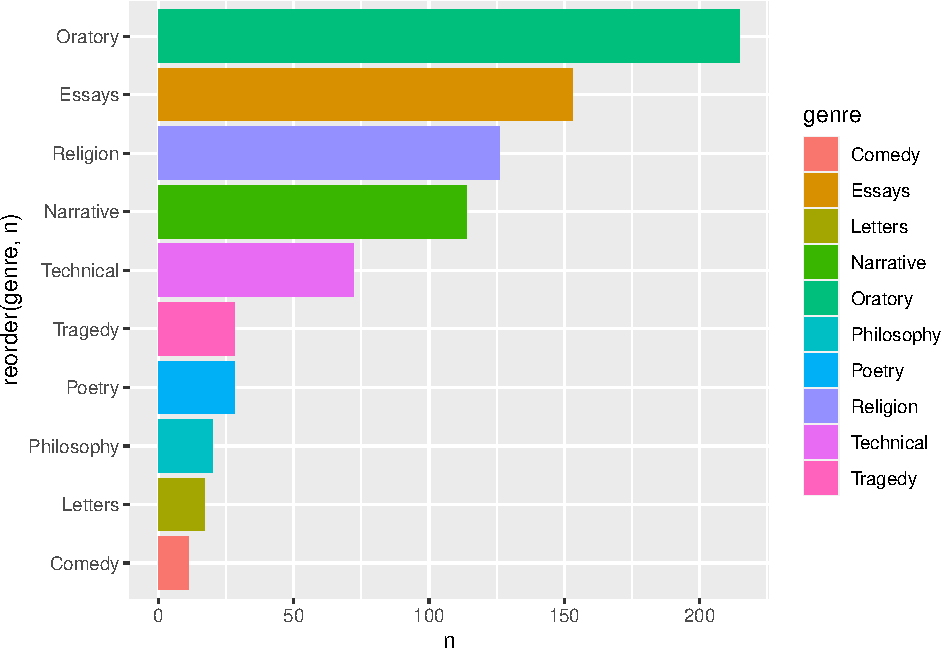
\includegraphics{_main_files/figure-latex/unnamed-chunk-48-1.pdf}

\textbf{Точечная диаграмма}, или dotplot, подходит для тех случаев, когда мы исследуем распределение наблюдений для разных групп данных, причем наблюдений не очень много. Например, мы можем отразить распределение текстов в корпусе по годам. Категориальную переменную (например, жанр) можно дополнительно закодировать цветом (\href{https://t.me/antibarbari/109}{Подробнее}).

\begin{Shaded}
\begin{Highlighting}[]
\NormalTok{diorisis\_meta }\SpecialCharTok{\%\textgreater{}\%} \FunctionTok{ggplot}\NormalTok{(}\FunctionTok{aes}\NormalTok{(date, }\AttributeTok{fill =} \FunctionTok{factor}\NormalTok{(genre))) }\SpecialCharTok{+} 
  \FunctionTok{geom\_dotplot}\NormalTok{(}\AttributeTok{binwidth =} \DecValTok{10}\NormalTok{, }\AttributeTok{stackdir =} \StringTok{"centerwhole"}\NormalTok{, }\AttributeTok{binpositions =} \StringTok{"all"}\NormalTok{) }\SpecialCharTok{+}  
  \FunctionTok{scale\_y\_continuous}\NormalTok{(}\ConstantTok{NULL}\NormalTok{, }\AttributeTok{breaks =} \ConstantTok{NULL}\NormalTok{) }\SpecialCharTok{+} 
  \FunctionTok{scale\_x\_continuous}\NormalTok{(}\AttributeTok{breaks =}\NormalTok{ scales}\SpecialCharTok{::}\FunctionTok{pretty\_breaks}\NormalTok{(}\AttributeTok{n =} \DecValTok{10}\NormalTok{))}
\end{Highlighting}
\end{Shaded}

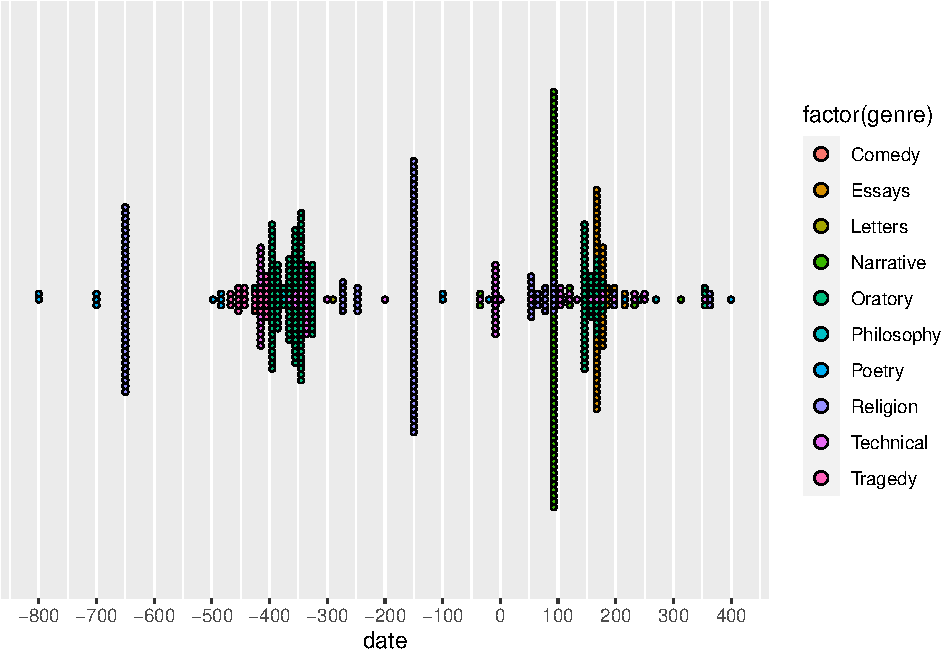
\includegraphics{_main_files/figure-latex/unnamed-chunk-49-1.pdf}

Различные группы данных можно выделять не только цветом и формой, но \textbf{Категоризованный график} -- отдельный график для разных групп. Попробуем выяснить: сколько поджанров в каждом жанре?

\begin{Shaded}
\begin{Highlighting}[]
\NormalTok{diorisis\_meta }\SpecialCharTok{\%\textgreater{}\%} 
  \FunctionTok{group\_by}\NormalTok{(genre, subgenre) }\SpecialCharTok{\%\textgreater{}\%} 
\NormalTok{  count }\SpecialCharTok{\%\textgreater{}\%}
  \FunctionTok{filter}\NormalTok{(genre }\SpecialCharTok{\%in\%} \FunctionTok{c}\NormalTok{(}\StringTok{"Poetry"}\NormalTok{, }\StringTok{"Technical"}\NormalTok{)) }\SpecialCharTok{\%\textgreater{}\%} 
  \FunctionTok{ggplot}\NormalTok{(}\FunctionTok{aes}\NormalTok{(}\FunctionTok{reorder}\NormalTok{(subgenre, n), n, }\AttributeTok{fill =}\NormalTok{ subgenre)) }\SpecialCharTok{+} 
  \FunctionTok{geom\_col}\NormalTok{(}\AttributeTok{show.legend =}\NormalTok{ F) }\SpecialCharTok{+}
  \FunctionTok{facet\_wrap}\NormalTok{(}\SpecialCharTok{\textasciitilde{}}\NormalTok{genre, }\AttributeTok{scales =} \StringTok{"free"}\NormalTok{) }\SpecialCharTok{+} \CommentTok{\# вот здесь задаем  группы}
  \FunctionTok{coord\_flip}\NormalTok{()}
\end{Highlighting}
\end{Shaded}

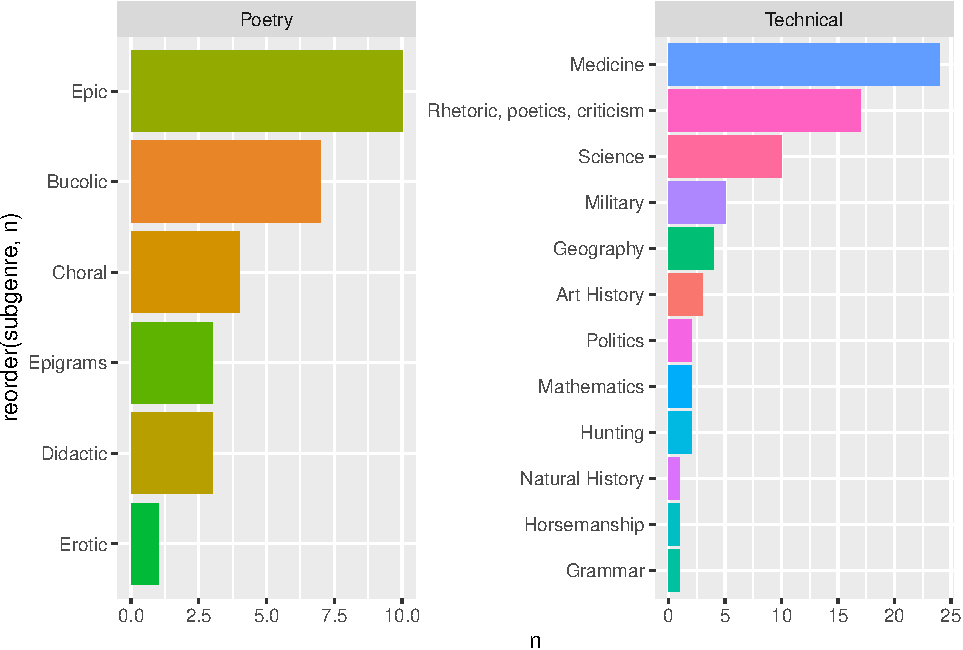
\includegraphics{_main_files/figure-latex/unnamed-chunk-50-1.pdf}

Подробнее с разными видами графиков мы познакомимся дальше.

\hypertarget{ux44dux43aux441ux43fux43eux440ux442-ux433ux440ux430ux444ux438ux43aux43eux432-ux438ux437-ux441ux440ux435ux434ux44b-r}{%
\section{Экспорт графиков из среды R}\label{ux44dux43aux441ux43fux43eux440ux442-ux433ux440ux430ux444ux438ux43aux43eux432-ux438ux437-ux441ux440ux435ux434ux44b-r}}

Способы:

\begin{itemize}
\tightlist
\item
  реализованные в R драйверы стандартных графических устройств;
\item
  функция \texttt{ggsave()}
\item
  меню программы RStudio.
\end{itemize}

\begin{Shaded}
\begin{Highlighting}[]
\CommentTok{\# код сохранит pdf в рабочую директорию }
\FunctionTok{pdf}\NormalTok{(}\AttributeTok{file =} \StringTok{"Diorisis.pdf"}\NormalTok{)}
\NormalTok{diorisis\_meta }\SpecialCharTok{\%\textgreater{}\%} 
  \FunctionTok{group\_by}\NormalTok{(genre, subgenre) }\SpecialCharTok{\%\textgreater{}\%} 
\NormalTok{  count }\SpecialCharTok{\%\textgreater{}\%}
  \FunctionTok{filter}\NormalTok{(genre }\SpecialCharTok{\%in\%} \FunctionTok{c}\NormalTok{(}\StringTok{"Poetry"}\NormalTok{, }\StringTok{"Technical"}\NormalTok{)) }\SpecialCharTok{\%\textgreater{}\%} 
  \FunctionTok{ggplot}\NormalTok{(}\FunctionTok{aes}\NormalTok{(}\FunctionTok{reorder}\NormalTok{(subgenre, n), n, }\AttributeTok{fill =}\NormalTok{ subgenre)) }\SpecialCharTok{+} 
  \FunctionTok{geom\_col}\NormalTok{(}\AttributeTok{show.legend =}\NormalTok{ F) }\SpecialCharTok{+}
  \FunctionTok{facet\_wrap}\NormalTok{(}\SpecialCharTok{\textasciitilde{}}\NormalTok{genre, }\AttributeTok{scales =} \StringTok{"free"}\NormalTok{) }\SpecialCharTok{+}
  \FunctionTok{coord\_flip}\NormalTok{()}
\FunctionTok{dev.off}\NormalTok{()}

\CommentTok{\# еще один способ сохранить последний график}
\FunctionTok{ggsave}\NormalTok{(}
  \AttributeTok{filename =} \StringTok{"Diorisis.png"}\NormalTok{,}
  \AttributeTok{plot =} \FunctionTok{last\_plot}\NormalTok{(),}
  \AttributeTok{device =} \StringTok{"png"}\NormalTok{,}
  \AttributeTok{scale =} \DecValTok{1}\NormalTok{,}
  \AttributeTok{width =} \ConstantTok{NA}\NormalTok{,}
  \AttributeTok{height =} \DecValTok{500}\NormalTok{,}
  \AttributeTok{units =} \StringTok{"px"}\NormalTok{,}
  \AttributeTok{dpi =} \DecValTok{300}
\NormalTok{)}
\end{Highlighting}
\end{Shaded}

\hypertarget{ux43eux43fux440ux44fux442ux43dux44bux435-ux434ux430ux43dux43dux44bux435}{%
\chapter{Опрятные данные}\label{ux43eux43fux440ux44fux442ux43dux44bux435-ux434ux430ux43dux43dux44bux435}}

\begin{quote}
Tidy datasets are all alike, but every messy dataset is messy in its own way.

--- Hadley Wickham
\end{quote}

\hypertarget{ux441ux438ux43dux442ux430ux43aux441ux438ux441-tidyverse}{%
\section{Синтаксис tidyverse}\label{ux441ux438ux43dux442ux430ux43aux441ux438ux441-tidyverse}}

Существуют два основных ``диалекта'' R, один из которых опирается главным образом на функции и структуры данных базового R, а другой пользуется синтаксисом tidyverse \citep{winter2020}. Tidyverse -- это семейство пакетов (\textbf{метапакет}), разработанных Хадли Уикхемом и др., которое включает в себя в том числе пакеты \texttt{dplyr}, \texttt{ggplot2} и многие другие.

\begin{Shaded}
\begin{Highlighting}[]
\CommentTok{\# загрузить все семейство}
\FunctionTok{library}\NormalTok{(tidyverse)}
\end{Highlighting}
\end{Shaded}

\hypertarget{tibble}{%
\subsection{Tibble}\label{tibble}}

Основная структура данных в tidyverse -- это tibble, современный вариант датафрейма\footnote{\url{https://r4ds.had.co.nz/tibbles.html}}. Тиббл, как говорят его разработчики, это ленивые и недовольные датафреймы: они делают меньше и жалуются больше\footnote{\url{https://tibble.tidyverse.org/}}. Это позволяет решать проблемы на более ранних этапах, что, как правило, приводит к созданию более чистого и выразительного кода.

Основные отличия от обычного датафрейма:

\begin{itemize}
\tightlist
\item
  текст по умолчанию конвертируется в строки, а не в факторы;\footnote{Подробнее о том, почему так вообще происходит: \url{https://simplystatistics.org/posts/2015-07-24-stringsasfactors-an-unauthorized-biography/}}
\item
  усовершенствованный метод \texttt{print()}, не нужно постоянно вызывать \texttt{head()};
\item
  нет имен рядов;
\item
  допускает синтаксически ``неправильные'' имена столбцов;
\item
  при индексировании не меняет тип данных на вектор и др.
\end{itemize}

\begin{Shaded}
\begin{Highlighting}[]
\FunctionTok{load}\NormalTok{(}\StringTok{"./datasets/DiorisisMeta.Rdata"}\NormalTok{)}

\CommentTok{\# распечатывает только первые 10 рядов, для каждого столбца указан тип данных, строки пронумерованы}
\FunctionTok{as\_tibble}\NormalTok{(diorisis\_meta)}
\end{Highlighting}
\end{Shaded}

\begin{verbatim}
## # A tibble: 784 x 5
##    name            title                      date genre     subgenre       
##    <chr>           <chr>                     <dbl> <chr>     <chr>          
##  1 Achilles Tatius Leucippe and Clitophon      120 Narrative Novel          
##  2 Aelian          De Natura Animalium         230 Technical Natural History
##  3 Aelian          Epistulae Rusticae          230 Letters   Letters        
##  4 Aelian          Varia Historia              200 Essays    Miscellanea    
##  5 Aeneas Tacticus Poliorcetica               -350 Technical Military       
##  6 Aeschines       Against Ctesiphon          -330 Oratory   Oratory        
##  7 Aeschines       Against Timarchus          -347 Oratory   Oratory        
##  8 Aeschines       The Speech on the Embassy  -336 Oratory   Oratory        
##  9 Aeschylus       Agamemnon                  -458 Tragedy   Tragedy        
## 10 Aeschylus       Eumenides                  -458 Tragedy   Tragedy        
## # i 774 more rows
\end{verbatim}

\begin{Shaded}
\begin{Highlighting}[]
\CommentTok{\# индексирование }
\FunctionTok{head}\NormalTok{(}\FunctionTok{as.data.frame}\NormalTok{(diorisis\_meta)[, }\DecValTok{1}\NormalTok{])  }\CommentTok{\# возвращает вектор}
\end{Highlighting}
\end{Shaded}

\begin{verbatim}
## [1] "Achilles Tatius" "Aelian"          "Aelian"          "Aelian"         
## [5] "Aeneas Tacticus" "Aeschines"
\end{verbatim}

\begin{Shaded}
\begin{Highlighting}[]
\FunctionTok{as\_tibble}\NormalTok{(diorisis\_meta)[,}\DecValTok{1}\NormalTok{] }\CommentTok{\# возвращает тиббл}
\end{Highlighting}
\end{Shaded}

\begin{verbatim}
## # A tibble: 784 x 1
##    name           
##    <chr>          
##  1 Achilles Tatius
##  2 Aelian         
##  3 Aelian         
##  4 Aelian         
##  5 Aeneas Tacticus
##  6 Aeschines      
##  7 Aeschines      
##  8 Aeschines      
##  9 Aeschylus      
## 10 Aeschylus      
## # i 774 more rows
\end{verbatim}

\begin{Shaded}
\begin{Highlighting}[]
\CommentTok{\# имена столбцов}
\NormalTok{df }\OtherTok{\textless{}{-}} \FunctionTok{data.frame}\NormalTok{(}\StringTok{\textquotesingle{}var 1\textquotesingle{}} \OtherTok{=} \DecValTok{1}\SpecialCharTok{:}\DecValTok{2}\NormalTok{, }\AttributeTok{two =} \DecValTok{3}\SpecialCharTok{:}\DecValTok{4}\NormalTok{)}
\NormalTok{df}
\end{Highlighting}
\end{Shaded}

\begin{verbatim}
##   var.1 two
## 1     1   3
## 2     2   4
\end{verbatim}

\begin{Shaded}
\begin{Highlighting}[]
\NormalTok{tbl }\OtherTok{\textless{}{-}} \FunctionTok{tibble}\NormalTok{(}\StringTok{\textquotesingle{}var 1\textquotesingle{}} \OtherTok{=} \DecValTok{1}\SpecialCharTok{:}\DecValTok{2}\NormalTok{, }\AttributeTok{two =} \DecValTok{3}\SpecialCharTok{:}\DecValTok{4}\NormalTok{)}
\NormalTok{tbl}
\end{Highlighting}
\end{Shaded}

\begin{verbatim}
## # A tibble: 2 x 2
##   `var 1`   two
##     <int> <int>
## 1       1     3
## 2       2     4
\end{verbatim}

\hypertarget{dplyr}{%
\subsection{Dplyr}\label{dplyr}}

Но самое главное, tibble подходит для ``грамматики манипуляции данных'', лежащей в основе \texttt{dplyr}\footnote{\url{https://dplyr.tidyverse.org/}}. Эта грамматика предоставляет последовательный набор глаголов, которые помогают решать наиболее распространенные задачи манипулирования данными:

\begin{itemize}
\tightlist
\item
  \texttt{mutate()} добавляет новые переменные, которые являются функциями существующих переменных;
\item
  \texttt{select()} выбирает переменные на основе их имен;
\item
  \texttt{filter()} выбирает наблюдения на основе их значений;
\item
  \texttt{summarise()} обобщает значения;
\item
  \texttt{arrange()} изменяет порядок следования строк.
\end{itemize}

Все эти глаголы естественным образом сочетаются с функцией \texttt{group\_by()}, которая позволяет выполнять любые операции ``по группам'', и с оператором \textbf{pipe} \texttt{\%\textgreater{}\%} из пакета \texttt{magrittr}.

В итоге получается более лаконичный и читаемый код, что можно показать на примере.

\begin{Shaded}
\begin{Highlighting}[]
\NormalTok{diorisis\_meta }\SpecialCharTok{\%\textgreater{}\%} 
  \FunctionTok{select}\NormalTok{(}\SpecialCharTok{{-}}\NormalTok{subgenre) }\SpecialCharTok{\%\textgreater{}\%} 
  \FunctionTok{filter}\NormalTok{(genre }\SpecialCharTok{==} \StringTok{"Narrative"}\NormalTok{) }\SpecialCharTok{\%\textgreater{}\%}  \CommentTok{\# не нужны кавычки!}
  \FunctionTok{group\_by}\NormalTok{(name) }\SpecialCharTok{\%\textgreater{}\%} 
  \FunctionTok{count}\NormalTok{() }\SpecialCharTok{\%\textgreater{}\%} 
  \FunctionTok{arrange}\NormalTok{(}\SpecialCharTok{{-}}\NormalTok{n)}
\end{Highlighting}
\end{Shaded}

\begin{verbatim}
## # A tibble: 20 x 2
## # Groups:   name [20]
##    name                           n
##    <chr>                      <int>
##  1 Plutarch                      71
##  2 Appian                        14
##  3 Flavius Josephus               4
##  4 Xenophon                       4
##  5 Arrian                         3
##  6 Diodorus Siculus               3
##  7 Philostratus the Athenian      2
##  8 Achilles Tatius                1
##  9 Cassius Dio                    1
## 10 Chariton                       1
## 11 Diogenes Laertius              1
## 12 Dionysius of Halicarnassus     1
## 13 Eusebius of Caesarea           1
## 14 Herodotus                      1
## 15 Longus                         1
## 16 Lucian                         1
## 17 Polybius                       1
## 18 Pseudo Apollodorus             1
## 19 Thucydides                     1
## 20 Xenophon of Ephesus            1
\end{verbatim}

В базовом R мы бы делали то же самое вот так:

\begin{Shaded}
\begin{Highlighting}[]
\NormalTok{diorisis\_df }\OtherTok{\textless{}{-}} \FunctionTok{as.data.frame}\NormalTok{(diorisis\_meta)}
\NormalTok{diorisis\_select }\OtherTok{\textless{}{-}}\NormalTok{ diorisis\_df[,}\SpecialCharTok{{-}}\DecValTok{5}\NormalTok{] }\CommentTok{\# remove column}
\NormalTok{diorisis\_filter }\OtherTok{\textless{}{-}}\NormalTok{ diorisis\_select[diorisis\_select}\SpecialCharTok{$}\NormalTok{genre }\SpecialCharTok{==} \StringTok{"Narrative"}\NormalTok{, ]}
\NormalTok{diorisis\_names }\OtherTok{\textless{}{-}}\NormalTok{ diorisis\_filter}\SpecialCharTok{$}\NormalTok{name}
\NormalTok{diorisis\_count }\OtherTok{\textless{}{-}} \FunctionTok{as.data.frame}\NormalTok{(}\FunctionTok{table}\NormalTok{(diorisis\_names))}
\NormalTok{diorisis\_sort }\OtherTok{\textless{}{-}}\NormalTok{ diorisis\_count[}\FunctionTok{order}\NormalTok{(diorisis\_count}\SpecialCharTok{$}\NormalTok{Freq, }\AttributeTok{decreasing =}\NormalTok{T),]}
\NormalTok{diorisis\_sort}
\end{Highlighting}
\end{Shaded}

\begin{verbatim}
##                diorisis_names Freq
## 15                   Plutarch   71
## 2                      Appian   14
## 10           Flavius Josephus    4
## 19                   Xenophon    4
## 3                      Arrian    3
## 6            Diodorus Siculus    3
## 14  Philostratus the Athenian    2
## 1             Achilles Tatius    1
## 4                 Cassius Dio    1
## 5                    Chariton    1
## 7           Diogenes Laertius    1
## 8  Dionysius of Halicarnassus    1
## 9        Eusebius of Caesarea    1
## 11                  Herodotus    1
## 12                     Longus    1
## 13                     Lucian    1
## 16                   Polybius    1
## 17         Pseudo Apollodorus    1
## 18                 Thucydides    1
## 20        Xenophon of Ephesus    1
\end{verbatim}

Тут должен быть какой-то поучительный вывод.

\hypertarget{ux43eux43fux440ux44fux442ux43dux44bux435-ux434ux430ux43dux43dux44bux435-1}{%
\section{Опрятные данные}\label{ux43eux43fux440ux44fux442ux43dux44bux435-ux434ux430ux43dux43dux44bux435-1}}

Но tidyverse -- это не только особый синтаксис, но и отдельная идеология ``опрятных данных''. ``Сырые'' данные, с которыми мы работаем, редко бывают опрятны, и перед анализом их следует ``почистить'' и преобразовать\footnote{\url{https://r4ds.had.co.nz/tidy-data.html}}.

Основные правила опрятных данных:

\begin{itemize}
\tightlist
\item
  отдельный столбец для каждой переменной;
\item
  отдельный ряд для каждого наблюдения;
\item
  у каждого значения отдельная ячейка;
\item
  один датасет -- одна таблица.
\end{itemize}

\textbf{Добавить картинку: принципы опрятных данных.}

Посмотрите на эти данные из пакета \texttt{tidyr} и подумайте, какое из этих правил нарушено в каждом случае.

\begin{Shaded}
\begin{Highlighting}[]
\FunctionTok{data}\NormalTok{(}\StringTok{"table2"}\NormalTok{)}
\NormalTok{table2}
\end{Highlighting}
\end{Shaded}

\begin{verbatim}
## # A tibble: 12 x 4
##    country      year type            count
##    <chr>       <dbl> <chr>           <dbl>
##  1 Afghanistan  1999 cases             745
##  2 Afghanistan  1999 population   19987071
##  3 Afghanistan  2000 cases            2666
##  4 Afghanistan  2000 population   20595360
##  5 Brazil       1999 cases           37737
##  6 Brazil       1999 population  172006362
##  7 Brazil       2000 cases           80488
##  8 Brazil       2000 population  174504898
##  9 China        1999 cases          212258
## 10 China        1999 population 1272915272
## 11 China        2000 cases          213766
## 12 China        2000 population 1280428583
\end{verbatim}

\begin{Shaded}
\begin{Highlighting}[]
\FunctionTok{data}\NormalTok{(}\StringTok{"table3"}\NormalTok{)}
\NormalTok{table3}
\end{Highlighting}
\end{Shaded}

\begin{verbatim}
## # A tibble: 6 x 3
##   country      year rate             
##   <chr>       <dbl> <chr>            
## 1 Afghanistan  1999 745/19987071     
## 2 Afghanistan  2000 2666/20595360    
## 3 Brazil       1999 37737/172006362  
## 4 Brazil       2000 80488/174504898  
## 5 China        1999 212258/1272915272
## 6 China        2000 213766/1280428583
\end{verbatim}

\begin{Shaded}
\begin{Highlighting}[]
\FunctionTok{data}\NormalTok{(}\StringTok{"table4a"}\NormalTok{)}
\NormalTok{table4a}
\end{Highlighting}
\end{Shaded}

\begin{verbatim}
## # A tibble: 3 x 3
##   country     `1999` `2000`
##   <chr>        <dbl>  <dbl>
## 1 Afghanistan    745   2666
## 2 Brazil       37737  80488
## 3 China       212258 213766
\end{verbatim}

\begin{Shaded}
\begin{Highlighting}[]
\FunctionTok{data}\NormalTok{(}\StringTok{"table4b"}\NormalTok{)}
\NormalTok{table4b}
\end{Highlighting}
\end{Shaded}

\begin{verbatim}
## # A tibble: 3 x 3
##   country         `1999`     `2000`
##   <chr>            <dbl>      <dbl>
## 1 Afghanistan   19987071   20595360
## 2 Brazil       172006362  174504898
## 3 China       1272915272 1280428583
\end{verbatim}

Важные функции для преобразования данных из пакета \texttt{tidyr}:\footnote{\url{https://tidyr.tidyverse.org/reference/index.html}}

\begin{itemize}
\tightlist
\item
  \texttt{separate()} делит один столбец на новые;
\item
  \texttt{unite()} объединяет столбцы;
\item
  \texttt{pivot\_longer()} удлиняет таблицу;
\item
  \texttt{pivot\_wider()} расширяет таблицу;
\item
  \texttt{drop\_na()} и \texttt{replace\_na()} указывают, что делать с NA и др.
\end{itemize}

Также упомянем функцию \texttt{distinct()} из \texttt{dplyr}, которая оставляет только уникальные наблюдения и предсталяет собой аналог базовой \texttt{unique()} для таблиц.

Кроме того, в \texttt{dplyr} есть полезное семейство функций \texttt{\_join}, позволяющих объединять данные в различных таблицах.\footnote{\url{https://r4ds.had.co.nz/relational-data.html}} Ниже мы потренируемся с ними работать.

\hypertarget{ux43fux440ux438ux43cux435ux440-ux431ux443ux43aux43aux440ux43eux441ux441ux438ux43dux433}{%
\section{Пример: буккроссинг}\label{ux43fux440ux438ux43cux435ux440-ux431ux443ux43aux43aux440ux43eux441ux441ux438ux43dux433}}

\hypertarget{ux441ux43cux43eux442ux440ux438ux43c-ux43dux430-ux434ux430ux43dux43dux44bux435}{%
\subsection{Смотрим на данные}\label{ux441ux43cux43eux442ux440ux438ux43c-ux43dux430-ux434ux430ux43dux43dux44bux435}}

Загрузим пример неопрятных данных и попробуем их преобразовать для анализа. \href{http://www2.informatik.uni-freiburg.de/~cziegler/BX/}{Book-Crossing} -- датасет с рейтингами миллионов книг и обезличенными демографическими данными о более 250 тысячах их читателей. Этот датасет хранится в трех разных таблицах.

\begin{Shaded}
\begin{Highlighting}[]
\FunctionTok{load}\NormalTok{(}\StringTok{"./datasets/BooksBX.Rdata"}\NormalTok{)}
\FunctionTok{load}\NormalTok{(}\StringTok{"./datasets/RatingsBX.Rdata"}\NormalTok{)}
\FunctionTok{load}\NormalTok{(}\StringTok{"./datasets/UsersBX.Rdata"}\NormalTok{)}

\NormalTok{ratings}
\end{Highlighting}
\end{Shaded}

\begin{verbatim}
## # A tibble: 493,813 x 3
##    `User-ID` ISBN       `Book-Rating`
##        <dbl> <chr>              <dbl>
##  1    276725 034545104X             0
##  2    276726 0155061224             5
##  3    276727 0446520802             0
##  4    276729 052165615X             3
##  5    276729 0521795028             6
##  6    276733 2080674722             0
##  7    276736 3257224281             8
##  8    276737 0600570967             6
##  9    276744 038550120X             7
## 10    276745 342310538             10
## # i 493,803 more rows
\end{verbatim}

\begin{Shaded}
\begin{Highlighting}[]
\NormalTok{users}
\end{Highlighting}
\end{Shaded}

\begin{verbatim}
## # A tibble: 246,666 x 3
##    `User-ID` Location                           Age  
##        <dbl> <chr>                              <chr>
##  1         1 nyc, new york, usa                 NULL 
##  2         2 stockton, california, usa          18   
##  3         3 moscow, yukon territory, russia    NULL 
##  4         4 porto, v.n.gaia, portugal          17   
##  5         5 farnborough, hants, united kingdom NULL 
##  6         6 santa monica, california, usa      61   
##  7         7 washington, dc, usa                NULL 
##  8         8 timmins, ontario, canada           NULL 
##  9         9 germantown, tennessee, usa         NULL 
## 10        10 albacete, wisconsin, spain         26   
## # i 246,656 more rows
\end{verbatim}

\begin{Shaded}
\begin{Highlighting}[]
\NormalTok{books}
\end{Highlighting}
\end{Shaded}

\begin{verbatim}
## # A tibble: 270,760 x 8
##    ISBN       `Book-Title`         `Book-Author` `Year-Of-Publication` Publisher
##    <chr>      <chr>                <chr>                         <dbl> <chr>    
##  1 0195153448 Classical Mythology  Mark P. O. M~                  2002 Oxford U~
##  2 0002005018 Clara Callan         Richard Bruc~                  2001 HarperFl~
##  3 0060973129 Decision in Normandy Carlo D'Este                   1991 HarperPe~
##  4 0374157065 Flu: The Story of t~ Gina Bari Ko~                  1999 Farrar S~
##  5 0393045218 The Mummies of Urum~ E. J. W. Bar~                  1999 W. W. No~
##  6 0399135782 The Kitchen God's W~ Amy Tan                        1991 Putnam P~
##  7 0425176428 What If?: The World~ Robert Cowley                  2000 Berkley ~
##  8 0671870432 PLEADING GUILTY      Scott Turow                    1993 Audiowor~
##  9 0679425608 Under the Black Fla~ David Cordin~                  1996 Random H~
## 10 074322678X Where You'll Find M~ Ann Beattie                    2002 Scribner 
## # i 270,750 more rows
## # i 3 more variables: `Image-URL-S` <chr>, `Image-URL-M` <chr>,
## #   `Image-URL-L` <chr>
\end{verbatim}

Что не так с этими данными?

\begin{itemize}
\tightlist
\item
  \texttt{users} содержит больше одного значения в столбце Location
\item
  много отсутствующих значений
\item
  данные вводятся самими пользователями через сайт \url{https://www.bookcrossing.com/} ; они могут содержать недостоверную информацию, см. напр. \texttt{moscow,\ yukon\ territory,\ russia} (Юкон -- это территория Канады).
\item
  Age представляет собой строку и др.
\end{itemize}

\begin{itemize}
\tightlist
\item
  Прежде чем начинать преобразование, надо сформулировать примерный вопрос и понять, что для нас важно, а что нет.
\end{itemize}

Например:
- Сколько читателей старше 30 лет пользуются сервисом в Австралии?
- В какие года опубликованы самые популярные книги?
- Кто популярнее у читателей, Роулинг или Толкин?
- Какой процент пользователей никогда не оставляет отзывы?
- Есть ли связь между возрастом и количеством оценок?
и т.п.

\begin{itemize}
\tightlist
\item
  Также надо понять, через какие переменные связаны эти таблицы.
\end{itemize}

Ответ: \texttt{ratings} и \texttt{books} связаны через переменную \texttt{isbn}, \texttt{ratings} и \texttt{users} связаны через переменную \texttt{User-ID}.

\hypertarget{ux442ux440ux430ux43dux441ux444ux43eux440ux43cux438ux440ux443ux435ux43c-ux434ux430ux43dux43dux44bux435}{%
\subsection{Трансформируем данные}\label{ux442ux440ux430ux43dux441ux444ux43eux440ux43cux438ux440ux443ux435ux43c-ux434ux430ux43dux43dux44bux435}}

Начнем с пользователей.

\begin{Shaded}
\begin{Highlighting}[]
\NormalTok{users\_separated }\OtherTok{\textless{}{-}}\NormalTok{ users }\SpecialCharTok{\%\textgreater{}\%} 
  \FunctionTok{mutate}\NormalTok{(}\AttributeTok{Age =} \FunctionTok{as.numeric}\NormalTok{(Age)) }\SpecialCharTok{\%\textgreater{}\%}
  \FunctionTok{filter}\NormalTok{(}\SpecialCharTok{!}\FunctionTok{is.na}\NormalTok{(Age))  }\SpecialCharTok{\%\textgreater{}\%} \CommentTok{\# drop\_na(Age) тоже решил бы нашу задачу}
  \FunctionTok{separate}\NormalTok{(Location, }\AttributeTok{into =} \FunctionTok{c}\NormalTok{(}\ConstantTok{NA}\NormalTok{, }\ConstantTok{NA}\NormalTok{, }\StringTok{"country"}\NormalTok{), }\AttributeTok{sep =} \StringTok{","}\NormalTok{)}

\NormalTok{users\_separated }\CommentTok{\# можно было бы не сохранять, но так нагляднее}
\end{Highlighting}
\end{Shaded}

\begin{verbatim}
## # A tibble: 148,869 x 3
##    `User-ID` country        Age
##        <dbl> <chr>        <dbl>
##  1         2 " usa"          18
##  2         4 " portugal"     17
##  3         6 " usa"          61
##  4        10 " spain"        26
##  5        11 " australia"    14
##  6        13 " spain"        26
##  7        18 " brazil"       25
##  8        19 ""              14
##  9        20 " usa"          19
## 10        21 " spain"        46
## # i 148,859 more rows
\end{verbatim}

Здесь можно сразу посмотреть, из каких стран и какого возраста пользователи.

\begin{Shaded}
\begin{Highlighting}[]
\NormalTok{users\_separated }\SpecialCharTok{\%\textgreater{}\%} 
  \FunctionTok{group\_by}\NormalTok{(country) }\SpecialCharTok{\%\textgreater{}\%}
  \FunctionTok{count}\NormalTok{() }\SpecialCharTok{\%\textgreater{}\%} 
  \FunctionTok{arrange}\NormalTok{(}\SpecialCharTok{{-}}\NormalTok{n)}
\end{Highlighting}
\end{Shaded}

\begin{verbatim}
## # A tibble: 543 x 2
## # Groups:   country [543]
##    country               n
##    <chr>             <int>
##  1 " usa"            67138
##  2 " united kingdom" 10935
##  3 " canada"          9877
##  4 " spain"           9505
##  5 " germany"         8016
##  6 " australia"       7824
##  7  <NA>              5914
##  8 " italy"           4754
##  9 " france"          2395
## 10 " portugal"        2175
## # i 533 more rows
\end{verbatim}

Последние ряды этого тибла выглядят достаточно причудливо:

\begin{Shaded}
\begin{Highlighting}[]
\NormalTok{users\_separated }\SpecialCharTok{\%\textgreater{}\%} 
  \FunctionTok{group\_by}\NormalTok{(country) }\SpecialCharTok{\%\textgreater{}\%}
  \FunctionTok{count}\NormalTok{() }\SpecialCharTok{\%\textgreater{}\%} 
  \FunctionTok{arrange}\NormalTok{(n)}
\end{Highlighting}
\end{Shaded}

\begin{verbatim}
## # A tibble: 543 x 2
## # Groups:   country [543]
##    country                    n
##    <chr>                  <int>
##  1 "  pasig city."            1
##  2 " &#20013;&#22269;"        1
##  3 " &#32654;&#22269;"        1
##  4 " 5057chadwick ct."        1
##  5 " 600 083"                 1
##  6 " \\n/a\\\""               1
##  7 " a new year is ahead"     1
##  8 " aberdeenshire"           1
##  9 " agusan del sur"          1
## 10 " alabama"                 1
## # i 533 more rows
\end{verbatim}

Здесь возможно несколько стратегий. Можно выбрать все ряды с названиями реальных стран либо (если это соответствует исследовательской задаче) какую-то одну страну. Можно и проигнорировать, если происхождение пользователей не так важно. Допустим, мы решаем сосредоточиться на Испании. Обратите внимание, что в название страны после разделения функцией \texttt{separate()} попали пробелы, и от них надо избавиться. Это делается при помощи регулярных выражений (о них в другой раз) и функции \texttt{mutate()}.

\begin{Shaded}
\begin{Highlighting}[]
\NormalTok{spain\_data }\OtherTok{\textless{}{-}}\NormalTok{ users\_separated }\SpecialCharTok{\%\textgreater{}\%}
  \FunctionTok{mutate}\NormalTok{(}\AttributeTok{country =} \FunctionTok{str\_replace\_all}\NormalTok{(country, }\AttributeTok{pattern =} \StringTok{"}\SpecialCharTok{\textbackslash{}\textbackslash{}}\StringTok{s+"}\NormalTok{, }\StringTok{""}\NormalTok{)) }\SpecialCharTok{\%\textgreater{}\%} \CommentTok{\# это означает, что пробел мы меняем на "ничто", т.е. убираем}
  \FunctionTok{filter}\NormalTok{(country }\SpecialCharTok{==} \StringTok{"spain"}\NormalTok{) }\SpecialCharTok{\%\textgreater{}\%} 
  \FunctionTok{group\_by}\NormalTok{(Age) }\SpecialCharTok{\%\textgreater{}\%}
  \FunctionTok{count}\NormalTok{() }\SpecialCharTok{\%\textgreater{}\%} 
  \FunctionTok{arrange}\NormalTok{(}\SpecialCharTok{{-}}\NormalTok{n)}

\NormalTok{spain\_data }
\end{Highlighting}
\end{Shaded}

\begin{verbatim}
## # A tibble: 86 x 2
## # Groups:   Age [86]
##      Age     n
##    <dbl> <int>
##  1    25   514
##  2    26   510
##  3    23   480
##  4    24   467
##  5    28   459
##  6    27   450
##  7    29   430
##  8    30   403
##  9    22   386
## 10    21   351
## # i 76 more rows
\end{verbatim}

Столбиковая диаграмма подходит для визуализации подобных данных:

\begin{Shaded}
\begin{Highlighting}[]
\NormalTok{spain\_data }\SpecialCharTok{\%\textgreater{}\%} 
  \FunctionTok{ggplot}\NormalTok{(}\FunctionTok{aes}\NormalTok{(Age, n)) }\SpecialCharTok{+} 
  \FunctionTok{geom\_bar}\NormalTok{(}\AttributeTok{stat =} \StringTok{"identity"}\NormalTok{, }\AttributeTok{col =} \StringTok{"blue"}\NormalTok{, }\AttributeTok{fill =} \StringTok{"white"}\NormalTok{) }\SpecialCharTok{+}
  \FunctionTok{theme\_bw}\NormalTok{()}
\end{Highlighting}
\end{Shaded}

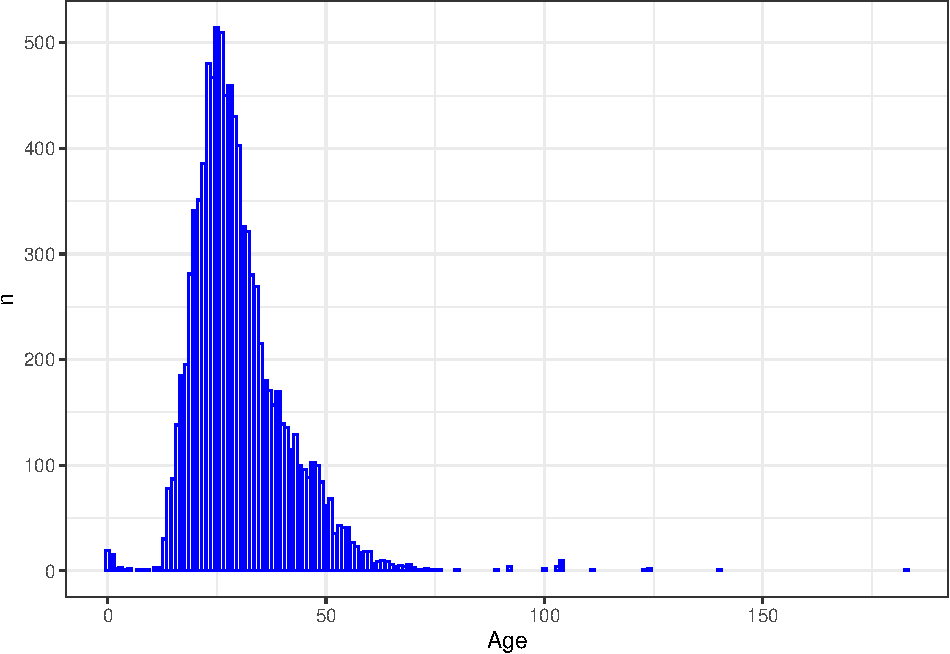
\includegraphics{_main_files/figure-latex/unnamed-chunk-63-1.pdf}

Какие целеустремленные испанцы! Читают от 0 до 183 лет 😵

После того, как мы убрали лишние пробелы из названий стран, можно фильтровать:

\begin{Shaded}
\begin{Highlighting}[]
\NormalTok{spain\_id }\OtherTok{\textless{}{-}}\NormalTok{ users\_separated }\SpecialCharTok{\%\textgreater{}\%}
  \FunctionTok{mutate}\NormalTok{(}\AttributeTok{country =} \FunctionTok{str\_replace\_all}\NormalTok{(country, }\AttributeTok{pattern =} \StringTok{"}\SpecialCharTok{\textbackslash{}\textbackslash{}}\StringTok{s+"}\NormalTok{, }\StringTok{""}\NormalTok{)) }\SpecialCharTok{\%\textgreater{}\%}
  \FunctionTok{filter}\NormalTok{(country }\SpecialCharTok{==} \StringTok{"spain"}\NormalTok{) }\CommentTok{\# на этот раз мы не считаем число наблюдений в группе, а забираем все ряды, которые отвечают условию}
\end{Highlighting}
\end{Shaded}

\hypertarget{ux43eux431ux44aux435ux434ux438ux43dux44fux435ux43c-ux434ux430ux43dux43dux44bux435}{%
\subsection{Объединяем данные}\label{ux43eux431ux44aux435ux434ux438ux43dux44fux435ux43c-ux434ux430ux43dux43dux44bux435}}

Мы уже выяснили, что \texttt{ratings} и \texttt{users} связаны через переменную \texttt{User-ID}, и в \texttt{ratings} хотели бы оставить только те id, которые отвечают заданному условию (страна, возраст и т.п.). Для такого рода объединений как раз подходят функции \texttt{\_join}\footnote{\url{https://r4ds.had.co.nz/relational-data.html}}.

\textbf{Добавить картинку на джойны.}

\begin{Shaded}
\begin{Highlighting}[]
\NormalTok{spain\_ratings }\OtherTok{\textless{}{-}}\NormalTok{ spain\_id }\SpecialCharTok{\%\textgreater{}\%} 
  \FunctionTok{left\_join}\NormalTok{(ratings) }\SpecialCharTok{\%\textgreater{}\%} 
  \FunctionTok{filter}\NormalTok{(}\SpecialCharTok{!}\FunctionTok{is.na}\NormalTok{(ISBN)) }\SpecialCharTok{\%\textgreater{}\%} 
  \FunctionTok{filter}\NormalTok{(}\StringTok{\textasciigrave{}}\AttributeTok{Book{-}Rating}\StringTok{\textasciigrave{}} \SpecialCharTok{\textgreater{}} \DecValTok{7}\NormalTok{) }\SpecialCharTok{\%\textgreater{}\%} \CommentTok{\# имена синтаксически неправильные, поэтому требуется знак "\textasciigrave{}"}
  \FunctionTok{group\_by}\NormalTok{(ISBN) }\SpecialCharTok{\%\textgreater{}\%} 
  \FunctionTok{count}\NormalTok{() }\SpecialCharTok{\%\textgreater{}\%} 
  \FunctionTok{arrange}\NormalTok{(}\SpecialCharTok{{-}}\NormalTok{n)}
\end{Highlighting}
\end{Shaded}

\begin{verbatim}
## Joining with `by = join_by(`User-ID`)`
\end{verbatim}

\begin{Shaded}
\begin{Highlighting}[]
\NormalTok{spain\_ratings}
\end{Highlighting}
\end{Shaded}

\begin{verbatim}
## # A tibble: 1,281 x 2
## # Groups:   ISBN [1,281]
##    ISBN           n
##    <chr>      <int>
##  1 8432206407     4
##  2 8433969978     4
##  3 846630679X     4
##  4 8472236552     4
##  5 8495501198     4
##  6 840149186X     3
##  7 8401499585     3
##  8 8423310353     3
##  9 8423662152     3
## 10 8432215007     3
## # i 1,271 more rows
\end{verbatim}

Осталось выяснить, что это за книги. Для этого объединяем \texttt{spain\_ratings} и \texttt{books}.

\begin{Shaded}
\begin{Highlighting}[]
\NormalTok{spain\_books }\OtherTok{\textless{}{-}}\NormalTok{ spain\_ratings }\SpecialCharTok{\%\textgreater{}\%} 
  \FunctionTok{filter}\NormalTok{(n }\SpecialCharTok{\textgreater{}} \DecValTok{2}\NormalTok{) }\SpecialCharTok{\%\textgreater{}\%} 
  \FunctionTok{left\_join}\NormalTok{(books) }\SpecialCharTok{\%\textgreater{}\%} 
  \FunctionTok{filter}\NormalTok{(}\SpecialCharTok{!}\FunctionTok{is.na}\NormalTok{(}\StringTok{\textasciigrave{}}\AttributeTok{Book{-}Title}\StringTok{\textasciigrave{}}\NormalTok{), }\SpecialCharTok{!}\FunctionTok{is.na}\NormalTok{(}\StringTok{\textasciigrave{}}\AttributeTok{Book{-}Author}\StringTok{\textasciigrave{}}\NormalTok{)) }\SpecialCharTok{\%\textgreater{}\%} 
  \FunctionTok{ungroup}\NormalTok{()}
\end{Highlighting}
\end{Shaded}

\begin{verbatim}
## Joining with `by = join_by(ISBN)`
\end{verbatim}

\begin{Shaded}
\begin{Highlighting}[]
\NormalTok{spain\_books}
\end{Highlighting}
\end{Shaded}

\begin{verbatim}
## # A tibble: 15 x 9
##    ISBN           n `Book-Title`   `Book-Author` `Year-Of-Publication` Publisher
##    <chr>      <int> <chr>          <chr>                         <dbl> <chr>    
##  1 8432206407     4 Sin Noticias ~ Eduardo Mend~                  1995 Planeta ~
##  2 8433969978     4 El Libro de L~ Paul Auster                    2003 Anagrama 
##  3 846630679X     4 La caverna = ~ Jose Saramago                  2002 Punto de~
##  4 8472236552     4 UN Viejo Que ~ Luis Sepulve~                  1993 Tusquets~
##  5 8495501198     4 Memorias de u~ Arthur Golden                  2001 Suma de ~
##  6 840149186X     3 El Club de Lo~ N. H. Kleinb~                  1995 Plaza &a~
##  7 8401499585     3 Los Pilares d~ Ken Follett                    1995 Plaza &a~
##  8 8423310353     3 El Camino (Co~ Miguel Delib~                  1991 Continen~
##  9 8432215007     3 El perfume     Patrick Susk~                  1997 Editoria~
## 10 8445071408     3 El Senor De L~ J. R. R. Tol~                  2001 Minotauro
## 11 8445071416     3 El Hobbit      J. R. R. Tol~                  1991 Minotauro
## 12 8477204055     3 El caballero ~ Robert Fisher                  2000 Obelisco 
## 13 8478884459     3 Harry Potter ~ J. K. Rowling                  1999 Lectorum~
## 14 8484602508     3 Diario de Un ~ Antonio Salas                  2003 Temas de~
## 15 8495501112     3 Son De Mar     Manuel Vicent                  2002 Suma de ~
## # i 3 more variables: `Image-URL-S` <chr>, `Image-URL-M` <chr>,
## #   `Image-URL-L` <chr>
\end{verbatim}

Как минимум мы выяснили, что испанцы предпочитают читать по испански! (Здесь снова можно подумать. Возможно, у одной книги разные ISBN, и стоило группировать не по ISBN, а по названию или автору?)

Осталось избавиться от неинформативных столбцов (это ссылки, часто битые, на изображения обложки). Если мы знаем номера этих столбцов, то это можно сделать по индексу:

\begin{Shaded}
\begin{Highlighting}[]
\NormalTok{spain\_books }\SpecialCharTok{\%\textgreater{}\%} 
  \FunctionTok{select}\NormalTok{(}\DecValTok{3}\SpecialCharTok{:}\DecValTok{5}\NormalTok{) }\SpecialCharTok{\%\textgreater{}\%} 
  \FunctionTok{rename}\NormalTok{(}\AttributeTok{title =} \StringTok{\textasciigrave{}}\AttributeTok{Book{-}Title}\StringTok{\textasciigrave{}}\NormalTok{, }\AttributeTok{author =} \StringTok{\textasciigrave{}}\AttributeTok{Book{-}Author}\StringTok{\textasciigrave{}}\NormalTok{)}
\end{Highlighting}
\end{Shaded}

\begin{verbatim}
## # A tibble: 15 x 3
##    title                                            author `Year-Of-Publication`
##    <chr>                                            <chr>                  <dbl>
##  1 Sin Noticias De Gurb (Biblioteca breve)          Eduar~                  1995
##  2 El Libro de Las Ilusiones                        Paul ~                  2003
##  3 La caverna = A caverna                           Jose ~                  2002
##  4 UN Viejo Que Leia Novelas De Amor/the Old Men W~ Luis ~                  1993
##  5 Memorias de una geisha                           Arthu~                  2001
##  6 El Club de Los Poetas Muertos                    N. H.~                  1995
##  7 Los Pilares de La Tierra                         Ken F~                  1995
##  8 El Camino (Coleccion Destinolibro)               Migue~                  1991
##  9 El perfume                                       Patri~                  1997
## 10 El Senor De Los Anillos: LA Comunidad Del Anill~ J. R.~                  2001
## 11 El Hobbit                                        J. R.~                  1991
## 12 El caballero de la armadura oxidada              Rober~                  2000
## 13 Harry Potter y la piedra filosofal               J. K.~                  1999
## 14 Diario de Un Skin: Un Topo En El Movimiento Neo~ Anton~                  2003
## 15 Son De Mar                                       Manue~                  2002
\end{verbatim}

Однако у \texttt{select()} есть функции-помощники\footnote{\url{https://r4ds.had.co.nz/transform.html}}, которые подходят для таких случаев:

\begin{itemize}
\tightlist
\item
  \texttt{starts\_with()}
\item
  \texttt{ends\_with()}
\item
  \texttt{contains()}
\item
  \texttt{matches()}
\item
  \texttt{num\_range()}
\end{itemize}

\begin{Shaded}
\begin{Highlighting}[]
\NormalTok{spain\_books }\SpecialCharTok{\%\textgreater{}\%} 
  \FunctionTok{select}\NormalTok{(}\SpecialCharTok{{-}}\FunctionTok{contains}\NormalTok{(}\StringTok{"URL"}\NormalTok{), }\SpecialCharTok{{-}}\FunctionTok{matches}\NormalTok{(}\StringTok{"Publisher"}\NormalTok{)) }\SpecialCharTok{\%\textgreater{}\%} \CommentTok{\# удалим заодно и издателя}
  \FunctionTok{rename}\NormalTok{(}\AttributeTok{title =} \StringTok{\textasciigrave{}}\AttributeTok{Book{-}Title}\StringTok{\textasciigrave{}}\NormalTok{, }
         \AttributeTok{author =} \StringTok{\textasciigrave{}}\AttributeTok{Book{-}Author}\StringTok{\textasciigrave{}}\NormalTok{,}
         \AttributeTok{published =} \StringTok{\textasciigrave{}}\AttributeTok{Year{-}Of{-}Publication}\StringTok{\textasciigrave{}}\NormalTok{) }\CommentTok{\# чиним имена}
\end{Highlighting}
\end{Shaded}

\begin{verbatim}
## # A tibble: 15 x 5
##    ISBN           n title                                       author published
##    <chr>      <int> <chr>                                       <chr>      <dbl>
##  1 8432206407     4 Sin Noticias De Gurb (Biblioteca breve)     Eduar~      1995
##  2 8433969978     4 El Libro de Las Ilusiones                   Paul ~      2003
##  3 846630679X     4 La caverna = A caverna                      Jose ~      2002
##  4 8472236552     4 UN Viejo Que Leia Novelas De Amor/the Old ~ Luis ~      1993
##  5 8495501198     4 Memorias de una geisha                      Arthu~      2001
##  6 840149186X     3 El Club de Los Poetas Muertos               N. H.~      1995
##  7 8401499585     3 Los Pilares de La Tierra                    Ken F~      1995
##  8 8423310353     3 El Camino (Coleccion Destinolibro)          Migue~      1991
##  9 8432215007     3 El perfume                                  Patri~      1997
## 10 8445071408     3 El Senor De Los Anillos: LA Comunidad Del ~ J. R.~      2001
## 11 8445071416     3 El Hobbit                                   J. R.~      1991
## 12 8477204055     3 El caballero de la armadura oxidada         Rober~      2000
## 13 8478884459     3 Harry Potter y la piedra filosofal          J. K.~      1999
## 14 8484602508     3 Diario de Un Skin: Un Topo En El Movimient~ Anton~      2003
## 15 8495501112     3 Son De Mar                                  Manue~      2002
\end{verbatim}

Возможно, сюда стоит добавить что-то про работу с факторами.

\hypertarget{ux444ux443ux43dux43aux446ux438ux43eux43dux430ux43bux44cux43dux43eux435-ux43fux440ux43eux433ux440ux430ux43cux43cux438ux440ux43eux432ux430ux43dux438ux435}{%
\chapter{Функциональное программирование}\label{ux444ux443ux43dux43aux446ux438ux43eux43dux430ux43bux44cux43dux43eux435-ux43fux440ux43eux433ux440ux430ux43cux43cux438ux440ux43eux432ux430ux43dux438ux435}}

\hypertarget{ux43dux430ux43fux438ux441ux430ux43dux438ux435-ux444ux443ux43dux43aux446ux438ux439}{%
\section{Написание функций}\label{ux43dux430ux43fux438ux441ux430ux43dux438ux435-ux444ux443ux43dux43aux446ux438ux439}}

Суть программирования на R сводится к написанию функций. Функция представляет собой набор команд, которые получают входные данные, используют их для вычисления других значений и возвращают результат \citep{мэтлофф2019}.

Чтобы определить функцию, необходимо дать ей имя, определить \textbf{формальные аргументы} и, при желании, \textbf{значения по умолчанию}. Тело функции пишется в фигурных скобках. В конце кода функции располагается команда \texttt{return()}; если ее нет, то функция возвращает последнее вычисленное значение (см. \href{https://r4ds.had.co.nz/functions.html}{здесь} о том, когда что предпочесть).

Напишем функцию, которая будет центрировать данные, то есть вычитать среднее из каждого значения:

\begin{Shaded}
\begin{Highlighting}[]
\NormalTok{center }\OtherTok{\textless{}{-}} \ControlFlowTok{function}\NormalTok{(x)\{ }
\NormalTok{  n }\OtherTok{=}\NormalTok{ x }\SpecialCharTok{{-}} \FunctionTok{mean}\NormalTok{(x)}
  \FunctionTok{return}\NormalTok{(n)}
\NormalTok{\}}

\NormalTok{x }\OtherTok{\textless{}{-}} \FunctionTok{c}\NormalTok{(}\DecValTok{5}\NormalTok{, }\DecValTok{10}\NormalTok{, }\DecValTok{15}\NormalTok{)}
\FunctionTok{center}\NormalTok{(x) }\CommentTok{\# это уже не формальный, а фактический аргумент}
\end{Highlighting}
\end{Shaded}

\begin{verbatim}
## [1] -5  0  5
\end{verbatim}

То же делает встроенная функция \texttt{scale()} (если значение аргумента \texttt{scale\ =\ F}; в противном случае разность дополнительно делится на стандартное отклонение, это называется стандартизация).

Внутри нашей функции есть переменная \texttt{n}, которую не видно в глобальном окружении. Это \textbf{локальная переменная}. Область ее видимости -- тело функции. Когда функция возвращает управление, переменная исчезает. Обратное неверно: глобальные переменные доступны в теле функции.

Функция может принимать произвольное число аргументов. Доработаем наш код:

\begin{Shaded}
\begin{Highlighting}[]
\NormalTok{center }\OtherTok{\textless{}{-}} \ControlFlowTok{function}\NormalTok{(x, }\AttributeTok{na.rm =}\NormalTok{ F)\{}
  \ControlFlowTok{if}\NormalTok{(na.rm) \{ x }\OtherTok{\textless{}{-}}\NormalTok{ x[}\SpecialCharTok{!}\FunctionTok{is.na}\NormalTok{(x)]\} }\CommentTok{\# добавим условие}
\NormalTok{  x }\SpecialCharTok{{-}} \FunctionTok{mean}\NormalTok{(x) }\CommentTok{\# на этот раз без return()}
\NormalTok{\}}

\NormalTok{x }\OtherTok{\textless{}{-}} \FunctionTok{c}\NormalTok{(}\DecValTok{5}\NormalTok{, }\DecValTok{10}\NormalTok{, }\ConstantTok{NA}\NormalTok{)}
\FunctionTok{center}\NormalTok{(x)}
\end{Highlighting}
\end{Shaded}

\begin{verbatim}
## [1] NA NA NA
\end{verbatim}

Что произошло? Почему следующий код выдает другой результат?

\begin{Shaded}
\begin{Highlighting}[]
\FunctionTok{center}\NormalTok{(x, }\AttributeTok{na.rm =}\NormalTok{ T)}
\end{Highlighting}
\end{Shaded}

\begin{verbatim}
## [1] -2.5  2.5
\end{verbatim}

Вычисления в R \textbf{ленивы}, то есть они откладываются до тех пор, пока не понадобится результат. Если вы зададите аргумент, который не нужен в теле функции, ошибки не будет.

\begin{Shaded}
\begin{Highlighting}[]
\NormalTok{center }\OtherTok{\textless{}{-}} \ControlFlowTok{function}\NormalTok{(x, }\AttributeTok{na.rm =}\NormalTok{ F, what\_is\_your\_name)\{}
  \ControlFlowTok{if}\NormalTok{(na.rm) \{ x }\OtherTok{\textless{}{-}}\NormalTok{ x[}\SpecialCharTok{!}\FunctionTok{is.na}\NormalTok{(x)]\} }\CommentTok{\# добавим условие}
\NormalTok{  x }\SpecialCharTok{{-}} \FunctionTok{mean}\NormalTok{(x) }\CommentTok{\# на этот раз без return()}
\NormalTok{\}}

\FunctionTok{center}\NormalTok{(x, }\AttributeTok{na.rm =}\NormalTok{ T)}
\end{Highlighting}
\end{Shaded}

\begin{verbatim}
## [1] -2.5  2.5
\end{verbatim}

\begin{Shaded}
\begin{Highlighting}[]
\FunctionTok{center}\NormalTok{(x, }\AttributeTok{na.rm =}\NormalTok{ T, }\AttributeTok{what\_is\_your\_name =} \StringTok{"Locusclassicus"}\NormalTok{)}
\end{Highlighting}
\end{Shaded}

\begin{verbatim}
## [1] -2.5  2.5
\end{verbatim}

Машине все равно, как вы назовете функцию, но тем, кто будет читать код, не все равно. Имена должны быть информативы (поэтому функция \texttt{f()} -- плохая идея). Также не стоит переписывать уже существующие в R имена!

Часто имеет смысл добавить условие остановки или сообщение, которое будет распечатано в консоль при выполнении.

\begin{Shaded}
\begin{Highlighting}[]
\NormalTok{center }\OtherTok{\textless{}{-}} \ControlFlowTok{function}\NormalTok{(x)\{}
  \ControlFlowTok{if}\NormalTok{ (}\FunctionTok{length}\NormalTok{(x) }\SpecialCharTok{==} \DecValTok{1}\NormalTok{) \{}\FunctionTok{stop}\NormalTok{(}\StringTok{"И без меня посчитает"}\NormalTok{)\}}
\NormalTok{  x }\SpecialCharTok{{-}} \FunctionTok{mean}\NormalTok{(x) }\CommentTok{\# на этот раз без return()}
\NormalTok{\}}

\NormalTok{x }\OtherTok{\textless{}{-}} \DecValTok{10}
\FunctionTok{center}\NormalTok{(x) }\CommentTok{\# вернет ошибку}
\end{Highlighting}
\end{Shaded}

Впрочем, в таких простых функциях в R нет необходимости. Сравните:

\begin{Shaded}
\begin{Highlighting}[]
\NormalTok{x }\OtherTok{\textless{}{-}} \FunctionTok{c}\NormalTok{(}\DecValTok{5}\NormalTok{, }\DecValTok{10}\NormalTok{, }\DecValTok{15}\NormalTok{)}
\NormalTok{x }\SpecialCharTok{{-}} \FunctionTok{mean}\NormalTok{(x)}
\end{Highlighting}
\end{Shaded}

\begin{verbatim}
## [1] -5  0  5
\end{verbatim}

\hypertarget{ux432ux435ux43aux442ux43eux440ux438ux437ux438ux440ux443ux439-ux44dux442ux43e}{%
\section{Векторизируй это}\label{ux432ux435ux43aux442ux43eux440ux438ux437ux438ux440ux443ux439-ux44dux442ux43e}}

Если имеется функция \texttt{f()}, которая должна быть применена ко всем элементам вектора \texttt{x}, то во многих случаях задача решается простым вызовом \texttt{f()} для самого вектора \texttt{x}. Это и есть векторизация. Она упрощает код и улучшает быстродействие.

Если функция R использует векторизованные операции, то она тоже является векторизованной \citep{мэтлофф2019}.

Это относится не только ко многим встроенным функциям R, но и к даже к операторам. \texttt{x\ +\ 4} в действительности представляет собой \texttt{+(x,\ 4)}:

\begin{Shaded}
\begin{Highlighting}[]
\NormalTok{x }\OtherTok{\textless{}{-}} \FunctionTok{c}\NormalTok{(}\FloatTok{1.2}\NormalTok{, }\FloatTok{2.51}\NormalTok{, }\FloatTok{3.8}\NormalTok{)}

\CommentTok{\# пример со встроенной функцией}
\FunctionTok{round}\NormalTok{(x)}
\end{Highlighting}
\end{Shaded}

\begin{verbatim}
## [1] 1 3 4
\end{verbatim}

\begin{Shaded}
\begin{Highlighting}[]
\CommentTok{\# пример с оператором}
\StringTok{\textasciigrave{}}\AttributeTok{+}\StringTok{\textasciigrave{}}\NormalTok{(x, }\DecValTok{4}\NormalTok{) }
\end{Highlighting}
\end{Shaded}

\begin{verbatim}
## [1] 5.20 6.51 7.80
\end{verbatim}

Ключевую роль здесь играет переработка данных, о которой мы уже говорили: короткий вектор повторяется до тех пор, пока его длина не сравняется с длиной более длинного вектора.

\begin{Shaded}
\begin{Highlighting}[]
\NormalTok{is\_article }\OtherTok{\textless{}{-}} \ControlFlowTok{function}\NormalTok{(x)\{}
\NormalTok{  x }\SpecialCharTok{==} \FunctionTok{c}\NormalTok{(}\StringTok{"a"}\NormalTok{, }\StringTok{"the"}\NormalTok{)}
\NormalTok{\}}

\NormalTok{x }\OtherTok{\textless{}{-}} \StringTok{"the"}
\FunctionTok{is\_article}\NormalTok{(x) }\CommentTok{\# возвращает два значения, хотя на входе было одно}
\end{Highlighting}
\end{Shaded}

\begin{verbatim}
## [1] FALSE  TRUE
\end{verbatim}

В двух примерах ниже векторы равной длины, но тут тоже есть особенность.

\begin{Shaded}
\begin{Highlighting}[]
\NormalTok{x }\OtherTok{\textless{}{-}} \FunctionTok{c}\NormalTok{(}\StringTok{"just"}\NormalTok{, }\StringTok{"the"}\NormalTok{)}
\FunctionTok{is\_article}\NormalTok{(x) }
\end{Highlighting}
\end{Shaded}

\begin{verbatim}
## [1] FALSE  TRUE
\end{verbatim}

\begin{Shaded}
\begin{Highlighting}[]
\NormalTok{x }\OtherTok{\textless{}{-}} \FunctionTok{c}\NormalTok{(}\StringTok{"the"}\NormalTok{, }\StringTok{"just"}\NormalTok{)}
\FunctionTok{is\_article}\NormalTok{(x) }\CommentTok{\# взрыв мозга}
\end{Highlighting}
\end{Shaded}

\begin{verbatim}
## [1] FALSE FALSE
\end{verbatim}

Почему так?

Внутри нашей функции вектор, а два вектора сравниваются поэлементно!

Получается, что для сравнения списка слов со списком артиклей нам надо переписать функцию. Например, так:

\begin{Shaded}
\begin{Highlighting}[]
\NormalTok{is\_article }\OtherTok{\textless{}{-}} \ControlFlowTok{function}\NormalTok{(x) \{ }
\NormalTok{  articles }\OtherTok{\textless{}{-}} \FunctionTok{c}\NormalTok{(}\StringTok{"a"}\NormalTok{, }\StringTok{"the"}\NormalTok{)}
\NormalTok{  x }\SpecialCharTok{\%in\%}\NormalTok{ articles}
\NormalTok{\}}

\NormalTok{x }\OtherTok{\textless{}{-}} \FunctionTok{c}\NormalTok{(}\FunctionTok{rep}\NormalTok{(}\StringTok{"the"}\NormalTok{, }\DecValTok{5}\NormalTok{), }\FunctionTok{rep}\NormalTok{(}\StringTok{"if"}\NormalTok{, }\DecValTok{5}\NormalTok{))}
\FunctionTok{is\_article}\NormalTok{(x)}
\end{Highlighting}
\end{Shaded}

\begin{verbatim}
##  [1]  TRUE  TRUE  TRUE  TRUE  TRUE FALSE FALSE FALSE FALSE FALSE
\end{verbatim}

\begin{Shaded}
\begin{Highlighting}[]
\FunctionTok{sum}\NormalTok{(}\FunctionTok{is\_article}\NormalTok{(x)) }
\end{Highlighting}
\end{Shaded}

\begin{verbatim}
## [1] 5
\end{verbatim}

\hypertarget{ux437ux430ux447ux435ux43c-ux43fux438ux441ux430ux442ux44c-ux444ux443ux43dux43aux446ux438ux438}{%
\section{Зачем писать функции?}\label{ux437ux430ux447ux435ux43c-ux43fux438ux441ux430ux442ux44c-ux444ux443ux43dux43aux446ux438ux438}}

Функции имеют три преимущества перед простой копипастой:

\begin{itemize}
\tightlist
\item
  у функции есть выразительное имя, которое облегчает понимание кода;
\item
  при изменении требований необходимо обновлять код только в одном месте, а не во многих;
\item
  меньше вероятность случайных ошибок при копировании (например, обновление имени переменной в одном месте, но не в другом)\href{https://r4ds.had.co.nz/functions.html}{подробнее}
\end{itemize}

Запомните простое правило: если вы трижды скопировали код, пора писать функцию!

\begin{quote}
Writing good functions is a lifetime journey.

--- Hadley Wickham
\end{quote}

Это не так сложно. Сначала пишем обычный код, потом превращаем его в функцию. Например, нам нужна функция, которая ищет совпадения в двух векторах и возвращает совпавшие элементы.

\begin{Shaded}
\begin{Highlighting}[]
\CommentTok{\# сначала решаем задачу для двух векторов}
\NormalTok{x }\OtherTok{\textless{}{-}} \FunctionTok{c}\NormalTok{(}\StringTok{"гнев"}\NormalTok{, }\StringTok{"богиня"}\NormalTok{, }\StringTok{"воспой"}\NormalTok{)}
\NormalTok{y }\OtherTok{\textless{}{-}} \FunctionTok{c}\NormalTok{(}\StringTok{"в"}\NormalTok{, }\StringTok{"мысли"}\NormalTok{, }\StringTok{"ему"}\NormalTok{, }\StringTok{"то"}\NormalTok{, }\StringTok{"вложила"}\NormalTok{, }\StringTok{"богиня"}\NormalTok{, }\StringTok{"державная"}\NormalTok{, }\StringTok{"гера"}\NormalTok{)}
\NormalTok{idx }\OtherTok{\textless{}{-}} \FunctionTok{which}\NormalTok{(x }\SpecialCharTok{\%in\%}\NormalTok{ y)}
\NormalTok{x[idx]}
\end{Highlighting}
\end{Shaded}

\begin{verbatim}
## [1] "богиня"
\end{verbatim}

\begin{Shaded}
\begin{Highlighting}[]
\CommentTok{\# потом упаковываем в функцию}
\NormalTok{common\_words }\OtherTok{\textless{}{-}} \ControlFlowTok{function}\NormalTok{(x, y)\{}
\NormalTok{  idx }\OtherTok{\textless{}{-}} \FunctionTok{which}\NormalTok{(x }\SpecialCharTok{\%in\%}\NormalTok{ y)}
\NormalTok{  x[idx]}
\NormalTok{\}}

\CommentTok{\# применяем к новым данным}
\NormalTok{x }\OtherTok{\textless{}{-}} \FunctionTok{c}\NormalTok{(}\StringTok{"лишь"}\NormalTok{, }\StringTok{"явилась"}\NormalTok{, }\StringTok{"заря"}\NormalTok{, }\StringTok{"розоперстая"}\NormalTok{, }\StringTok{"вестница"}\NormalTok{, }\StringTok{"утра"}\NormalTok{)}
\NormalTok{y }\OtherTok{\textless{}{-}} \FunctionTok{c}\NormalTok{(}\StringTok{"вестница"}\NormalTok{, }\StringTok{"утра"}\NormalTok{, }\StringTok{"заря"}\NormalTok{, }\StringTok{"на"}\NormalTok{, }\StringTok{"великий"}\NormalTok{, }\StringTok{"олимп"}\NormalTok{, }\StringTok{"восходила"}\NormalTok{)}
\FunctionTok{common\_words}\NormalTok{(x, y)}
\end{Highlighting}
\end{Shaded}

\begin{verbatim}
## [1] "заря"     "вестница" "утра"
\end{verbatim}

И ура, все работает!

Кроме того, очень полезно читать чужой код (если он хорошо написан). Начинку функции можно распечатать в консоль, если ввести ее название без скобок. Ниже код функции из пакета \texttt{Stylo}; эта функция отвечает за вычисление знаменитой Delta Берроуза. Попробуйте понять, что она делает.

\begin{Shaded}
\begin{Highlighting}[]
\FunctionTok{library}\NormalTok{(stylo)}
\NormalTok{dist.delta}
\end{Highlighting}
\end{Shaded}

\begin{verbatim}
## function (x, scale = TRUE) 
## {
##     if (is.matrix(x) == FALSE & is.data.frame(x) == FALSE) {
##         stop("cannot apply a distance measure: wrong data format!")
##     }
##     if (length(x[1, ]) < 2 | length(x[, 1]) < 2) {
##         stop("at least 2 cols and 2 rows are needed to compute a distance!")
##     }
##     if (scale == TRUE) {
##         x = scale(x)
##     }
##     y = dist(x, method = "manhattan")/length(x[1, ])
##     return(y)
## }
## <bytecode: 0x141bb3f58>
## <environment: namespace:stylo>
\end{verbatim}

\hypertarget{ux432ux435ux43aux442ux43eux440ux438ux437ux43eux432ux430ux43dux43dux44bux435-ux43aux43eux43dux441ux442ux440ux443ux43aux446ux438ux438}{%
\section{Векторизованные конструкции}\label{ux432ux435ux43aux442ux43eux440ux438ux437ux43eux432ux430ux43dux43dux44bux435-ux43aux43eux43dux441ux442ux440ux443ux43aux446ux438ux438}}

\hypertarget{ux446ux438ux43aux43bux44b}{%
\subsection{Циклы}\label{ux446ux438ux43aux43bux44b}}

Еще один способ повторить действия в R, при этом не копируя один и тот же код много раз, -- это циклы.

\begin{quote}
Один из главных принципов программирования на R гласит, что следует обходиться без циклов, а если это невозможно, то циклы должны быть простыми.

--- Нормат Мэтлофф
\end{quote}

Существует два основных цикла: цикл \texttt{for} и цикл \texttt{while}. На практике чаще используется цикл \texttt{for}, потому что цикл \texttt{while} легко отправить в бесконечность.

\hypertarget{ux446ux438ux43aux43b-for}{%
\subsubsection{\texorpdfstring{Цикл \texttt{for}}{Цикл for}}\label{ux446ux438ux43aux43b-for}}

Цикл ниже считает количество букв для каждого слова в векторе.

\begin{Shaded}
\begin{Highlighting}[]
\NormalTok{y }\OtherTok{\textless{}{-}} \FunctionTok{c}\NormalTok{(}\StringTok{"в"}\NormalTok{, }\StringTok{"мысли"}\NormalTok{, }\StringTok{"ему"}\NormalTok{, }\StringTok{"то"}\NormalTok{, }\StringTok{"вложила"}\NormalTok{, }\StringTok{"богиня"}\NormalTok{, }\StringTok{"державная"}\NormalTok{, }\StringTok{"гера"}\NormalTok{)}

\NormalTok{result }\OtherTok{\textless{}{-}} \FunctionTok{c}\NormalTok{()}
\ControlFlowTok{for}\NormalTok{(i }\ControlFlowTok{in}\NormalTok{ y) \{ }
\NormalTok{  n }\OtherTok{\textless{}{-}} \FunctionTok{nchar}\NormalTok{(i)}
\NormalTok{  result }\OtherTok{\textless{}{-}} \FunctionTok{c}\NormalTok{(result, n)}
\NormalTok{\}}

\NormalTok{result}
\end{Highlighting}
\end{Shaded}

\begin{verbatim}
## [1] 1 5 3 2 7 6 9 4
\end{verbatim}

В данном случае мы указали, что надо совершить какую-то операцию над каждым элементом вектора; но по сути это избыточно, потому что \texttt{nchar()} тоже векторизована.

\begin{Shaded}
\begin{Highlighting}[]
\FunctionTok{nchar}\NormalTok{(y)}
\end{Highlighting}
\end{Shaded}

\begin{verbatim}
## [1] 1 5 3 2 7 6 9 4
\end{verbatim}

Поэтому чаще цикл \texttt{for} применяют к другим структурам данных. Например, к спискам и датафреймам (хотя и этого можно избежать, о чем будет сказано дальше). Загрузим и немного изменим датасет о гапаксах у Платона. Изменения нужны, так как цикл работает для данных только одного вида.

\begin{Shaded}
\begin{Highlighting}[]
\FunctionTok{rownames}\NormalTok{(hapax\_plato) }\OtherTok{\textless{}{-}}\NormalTok{ hapax\_plato}\SpecialCharTok{$}\NormalTok{dialogue}
\NormalTok{hapax\_plato }\OtherTok{\textless{}{-}}\NormalTok{ hapax\_plato }\SpecialCharTok{\%\textgreater{}\%} \FunctionTok{select}\NormalTok{(}\SpecialCharTok{{-}}\NormalTok{ratio, }\SpecialCharTok{{-}}\NormalTok{group, }\SpecialCharTok{{-}}\NormalTok{dialogue) }\CommentTok{\# оператор pipe и функции из dplyr работают и с обычными датафреймами!}
\FunctionTok{str}\NormalTok{(hapax\_plato)}
\end{Highlighting}
\end{Shaded}

\begin{verbatim}
## 'data.frame':    26 obs. of  2 variables:
##  $ words: chr  "8745" "8311" "17944" "4950" ...
##  $ hapax: chr  "36" "31" "122" "104" ...
\end{verbatim}

Сейчас данные в нашей таблице имеют тип \texttt{chr}, то есть строка, и при помощи цикла мы можем их трансформировать.

\begin{Shaded}
\begin{Highlighting}[]
\ControlFlowTok{for}\NormalTok{ (i }\ControlFlowTok{in} \FunctionTok{seq\_along}\NormalTok{(hapax\_plato)) \{  }\CommentTok{\# seq\_along ≈ 1:length(x)}
\NormalTok{  hapax\_plato[,i] }\OtherTok{\textless{}{-}} \FunctionTok{as.numeric}\NormalTok{(hapax\_plato[,i])}
\NormalTok{\}}

\FunctionTok{str}\NormalTok{(hapax\_plato) }\CommentTok{\# убеждаемся, что все получилось}
\end{Highlighting}
\end{Shaded}

\begin{verbatim}
## 'data.frame':    26 obs. of  2 variables:
##  $ words: num  8745 8311 17944 4950 4169 ...
##  $ hapax: num  36 31 122 104 19 87 15 125 12 32 ...
\end{verbatim}

При помощи циклов можно не только трансформировать данные, но и создавать новые. Чтобы посчитать среднее для столбца, цикл писать не надо: для этого есть функция \texttt{colSums()} (или, для других задач, \texttt{rowSums()}). А вот посчитать медиану таким образом не получится, тут может пригодиться цикл.

\begin{Shaded}
\begin{Highlighting}[]
\NormalTok{medians }\OtherTok{\textless{}{-}} \FunctionTok{c}\NormalTok{()}
\ControlFlowTok{for}\NormalTok{ (i }\ControlFlowTok{in} \FunctionTok{seq\_along}\NormalTok{(hapax\_plato)) \{ }
\NormalTok{  m }\OtherTok{\textless{}{-}} \FunctionTok{median}\NormalTok{(hapax\_plato[,i])}
\NormalTok{  medians }\OtherTok{\textless{}{-}} \FunctionTok{c}\NormalTok{(medians, m)}
\NormalTok{\}}

\NormalTok{medians}
\end{Highlighting}
\end{Shaded}

\begin{verbatim}
## [1] 15589.5    94.5
\end{verbatim}

Мы сохранили результат, инициировав пустой вектор, к которому затем привязали данные по каждому столбцу. Это не всегда хорошая идея, поскольку для больших данных может сильно замедлить цикл\footnote{\url{https://r4ds.had.co.nz/iteration.html}}. Еще один способ -- сразу инициировать вектор нужной длины.

\begin{Shaded}
\begin{Highlighting}[]
\NormalTok{medians }\OtherTok{\textless{}{-}} \FunctionTok{vector}\NormalTok{(}\StringTok{"double"}\NormalTok{, }\FunctionTok{ncol}\NormalTok{(hapax\_plato))}
\ControlFlowTok{for}\NormalTok{ (i }\ControlFlowTok{in} \FunctionTok{seq\_along}\NormalTok{(hapax\_plato)) \{ }
\NormalTok{  medians[i] }\OtherTok{\textless{}{-}} \FunctionTok{median}\NormalTok{(hapax\_plato[,i])}
\NormalTok{\}}

\NormalTok{medians}
\end{Highlighting}
\end{Shaded}

\begin{verbatim}
## [1] 15589.5    94.5
\end{verbatim}

Сравнить скорость можно при помощи пакета \texttt{tictoc}.

\begin{Shaded}
\begin{Highlighting}[]
\FunctionTok{library}\NormalTok{(tictoc)}

\CommentTok{\# способ первый }
\FunctionTok{tic}\NormalTok{()}
\NormalTok{medians }\OtherTok{\textless{}{-}} \FunctionTok{c}\NormalTok{()}
\ControlFlowTok{for}\NormalTok{ (i }\ControlFlowTok{in} \FunctionTok{seq\_along}\NormalTok{(hapax\_plato)) \{ }
\NormalTok{  m }\OtherTok{\textless{}{-}} \FunctionTok{median}\NormalTok{(hapax\_plato[,i])}
\NormalTok{  medians }\OtherTok{\textless{}{-}} \FunctionTok{c}\NormalTok{(medians, m)}
\NormalTok{\}}
\FunctionTok{toc}\NormalTok{()}
\end{Highlighting}
\end{Shaded}

\begin{verbatim}
## 0.003 sec elapsed
\end{verbatim}

\begin{Shaded}
\begin{Highlighting}[]
\CommentTok{\# способ второй}
\FunctionTok{tic}\NormalTok{()}
\NormalTok{medians }\OtherTok{\textless{}{-}} \FunctionTok{vector}\NormalTok{(}\StringTok{"double"}\NormalTok{, }\FunctionTok{ncol}\NormalTok{(hapax\_plato))}
\ControlFlowTok{for}\NormalTok{ (i }\ControlFlowTok{in} \FunctionTok{seq\_along}\NormalTok{(hapax\_plato)) \{ }
\NormalTok{  medians[i] }\OtherTok{\textless{}{-}} \FunctionTok{median}\NormalTok{(hapax\_plato[,i])}
\NormalTok{\}}
\FunctionTok{toc}\NormalTok{()}
\end{Highlighting}
\end{Shaded}

\begin{verbatim}
## 0.003 sec elapsed
\end{verbatim}

Второй способ чуть быстрее, и для больших данных это может быть существенно (знала бы я это раньше).

Вы уже заметили, что в циклах часто используется буква \texttt{i}. Но никакой особой магии в ней нет!

\hypertarget{ux446ux438ux43aux43b-while}{%
\subsubsection{\texorpdfstring{Цикл \texttt{while}}{Цикл while}}\label{ux446ux438ux43aux43b-while}}

Как уже говорилось, с циклами \texttt{while} стоит быть осторожнее. Посмотрите, например, на этот цикл, который перебирает слова, пока не найдет слово длиной 6 букв. Что могло пойти не так?

\begin{Shaded}
\begin{Highlighting}[]
\NormalTok{k }\OtherTok{\textless{}{-}} \DecValTok{0}
\NormalTok{n }\OtherTok{\textless{}{-}} \DecValTok{0}
\ControlFlowTok{while}\NormalTok{ (n }\SpecialCharTok{!=} \DecValTok{6}\NormalTok{) \{}
\NormalTok{  k }\OtherTok{\textless{}{-}}\NormalTok{ k }\SpecialCharTok{+} \DecValTok{1}
\NormalTok{  n }\OtherTok{\textless{}{-}} \FunctionTok{nchar}\NormalTok{(y[k])}
\NormalTok{\}}

\NormalTok{y[k]}
\end{Highlighting}
\end{Shaded}

\begin{verbatim}
## [1] "богиня"
\end{verbatim}

То же самое можно сделать без цикла. Если подходящего значения не найдется, нам вернется \texttt{NA}.

\begin{Shaded}
\begin{Highlighting}[]
\NormalTok{y[}\FunctionTok{nchar}\NormalTok{(y) }\SpecialCharTok{==} \DecValTok{6}\NormalTok{][}\DecValTok{1}\NormalTok{] }
\end{Highlighting}
\end{Shaded}

\begin{verbatim}
## [1] "богиня"
\end{verbatim}

\hypertarget{ux443ux441ux43bux43eux432ux438ux44f}{%
\subsection{Условия}\label{ux443ux441ux43bux43eux432ux438ux44f}}

Задействуются в тех случаях, когда выполнение функции ограничивается неким условием.

\begin{Shaded}
\begin{Highlighting}[]
\ControlFlowTok{if}\NormalTok{(}\FunctionTok{any}\NormalTok{(}\FunctionTok{nchar}\NormalTok{(y) }\SpecialCharTok{\textgreater{}} \DecValTok{6}\NormalTok{)) }\FunctionTok{print}\NormalTok{(}\StringTok{"многабукв"}\NormalTok{)}
\end{Highlighting}
\end{Shaded}

\begin{verbatim}
## [1] "многабукв"
\end{verbatim}

Внутри условия не надо использовать логические операторы \texttt{\textbar{}} (``или'') или \texttt{\&} (``и''), потому что они векторизованы:

\begin{Shaded}
\begin{Highlighting}[]
\NormalTok{y}
\end{Highlighting}
\end{Shaded}

\begin{verbatim}
## [1] "в"         "мысли"     "ему"       "то"        "вложила"   "богиня"   
## [7] "державная" "гера"
\end{verbatim}

\begin{Shaded}
\begin{Highlighting}[]
\FunctionTok{nchar}\NormalTok{(y) }\SpecialCharTok{\textgreater{}} \DecValTok{6} \SpecialCharTok{|} \FunctionTok{nchar}\NormalTok{(y) }\SpecialCharTok{\textless{}} \DecValTok{2}
\end{Highlighting}
\end{Shaded}

\begin{verbatim}
## [1]  TRUE FALSE FALSE FALSE  TRUE FALSE  TRUE FALSE
\end{verbatim}

Вместо этого можно применять \texttt{\textbar{}\textbar{}} (``или'') или \texttt{\&\&} (``и''), которые остановятся, дойдя до первого истинного значения.

\begin{Shaded}
\begin{Highlighting}[]
\FunctionTok{nchar}\NormalTok{(y) }\SpecialCharTok{\textgreater{}} \DecValTok{6} \SpecialCharTok{||} \FunctionTok{nchar}\NormalTok{(y) }\SpecialCharTok{\textless{}} \DecValTok{2} 
\end{Highlighting}
\end{Shaded}

\begin{verbatim}
## [1] TRUE
\end{verbatim}

Множественные условия задаются так:

\begin{Shaded}
\begin{Highlighting}[]
\ControlFlowTok{if}\NormalTok{ (}\FunctionTok{sum}\NormalTok{(}\FunctionTok{nchar}\NormalTok{(y)) }\SpecialCharTok{\textgreater{}} \DecValTok{10}\NormalTok{) \{}
  \FunctionTok{print}\NormalTok{(}\StringTok{"много букв"}\NormalTok{)}
\NormalTok{\} }\ControlFlowTok{else} \ControlFlowTok{if}\NormalTok{ (}\FunctionTok{sum}\NormalTok{(}\FunctionTok{nchar}\NormalTok{(y)) }\SpecialCharTok{\textless{}} \DecValTok{5}\NormalTok{) \{}
  \FunctionTok{print}\NormalTok{(}\StringTok{"мало букв"}\NormalTok{)}
\NormalTok{\} }\ControlFlowTok{else}\NormalTok{ \{}
  \FunctionTok{print}\NormalTok{(}\StringTok{"норм букв"}\NormalTok{)}
\NormalTok{\}}
\end{Highlighting}
\end{Shaded}

\begin{verbatim}
## [1] "много букв"
\end{verbatim}

Но можно и короче:

\begin{Shaded}
\begin{Highlighting}[]
\FunctionTok{ifelse}\NormalTok{((}\FunctionTok{sum}\NormalTok{(}\FunctionTok{nchar}\NormalTok{(y)) }\SpecialCharTok{\textgreater{}} \DecValTok{10}\NormalTok{), }\StringTok{"много букв"}\NormalTok{, }\StringTok{"мало букв"}\NormalTok{)}
\end{Highlighting}
\end{Shaded}

\begin{verbatim}
## [1] "много букв"
\end{verbatim}

\hypertarget{ux441ux435ux43cux435ux439ux441ux442ux432ux43e-ux444ux443ux43dux43aux446ux438ux439-_apply-ux438ux437-ux431ux430ux437ux43eux432ux43eux433ux43e-r}{%
\section{Семейство функций \_apply из базового R}\label{ux441ux435ux43cux435ux439ux441ux442ux432ux43e-ux444ux443ux43dux43aux446ux438ux439-_apply-ux438ux437-ux431ux430ux437ux43eux432ux43eux433ux43e-r}}

Как уже было сказано, лучше обойтись без циклов, для этого в базовом R есть семейство функций \_apply.

\hypertarget{tapply}{%
\subsection{tapply()}\label{tapply}}

Принимает на входе вектор, фактор (или список факторов) и функцию. Каждый фактор должен быть той же длины, что и вектор.

\begin{Shaded}
\begin{Highlighting}[]
\FunctionTok{load}\NormalTok{(}\StringTok{"./datasets/HapaxPlato.Rdata"}\NormalTok{)}
\end{Highlighting}
\end{Shaded}

\begin{Shaded}
\begin{Highlighting}[]
\NormalTok{my\_fct }\OtherTok{\textless{}{-}} \FunctionTok{as.factor}\NormalTok{(hapax\_plato}\SpecialCharTok{$}\NormalTok{group)}
\NormalTok{my\_vct }\OtherTok{\textless{}{-}} \FunctionTok{as.numeric}\NormalTok{(hapax\_plato}\SpecialCharTok{$}\NormalTok{ratio)}
\FunctionTok{tapply}\NormalTok{(my\_vct, my\_fct, mean)}
\end{Highlighting}
\end{Shaded}

\begin{verbatim}
##          1          2          3 
## 0.00550000 0.00750000 0.01133333
\end{verbatim}

На диалекте tidyverse эта задача решается так:

\begin{Shaded}
\begin{Highlighting}[]
\NormalTok{hapax\_plato }\SpecialCharTok{\%\textgreater{}\%} 
  \FunctionTok{mutate}\NormalTok{(}\AttributeTok{ratio =} \FunctionTok{as.numeric}\NormalTok{(ratio)) }\SpecialCharTok{\%\textgreater{}\%} 
  \FunctionTok{group\_by}\NormalTok{(group) }\SpecialCharTok{\%\textgreater{}\%} 
  \FunctionTok{summarise}\NormalTok{(}\AttributeTok{mean =} \FunctionTok{mean}\NormalTok{(ratio))}
\end{Highlighting}
\end{Shaded}

\begin{verbatim}
## # A tibble: 3 x 2
##   group   mean
##   <dbl>  <dbl>
## 1     1 0.0055
## 2     2 0.0075
## 3     3 0.0113
\end{verbatim}

\hypertarget{apply}{%
\subsection{apply()}\label{apply}}

Вызывает функцию для каждой строки или столбца матрицы или датафрейма.

\begin{Shaded}
\begin{Highlighting}[]
\CommentTok{\# переносим названия диалогов в названия рядов}
\FunctionTok{rownames}\NormalTok{(hapax\_plato) }\OtherTok{\textless{}{-}}\NormalTok{ hapax\_plato}\SpecialCharTok{$}\NormalTok{dialogue}
\NormalTok{hapax\_plato }\OtherTok{\textless{}{-}} \FunctionTok{subset}\NormalTok{(hapax\_plato, }\AttributeTok{select =} \SpecialCharTok{{-}}\FunctionTok{c}\NormalTok{(dialogue, group)) }\CommentTok{\# еще один способ убрать столбцы}

\CommentTok{\# уточним вид данных по столбцам}
\FunctionTok{str}\NormalTok{(hapax\_plato)}
\end{Highlighting}
\end{Shaded}

\begin{verbatim}
## 'data.frame':    26 obs. of  3 variables:
##  $ words: chr  "8745" "8311" "17944" "4950" ...
##  $ hapax: chr  "36" "31" "122" "104" ...
##  $ ratio: chr  "0.004" "0.004" "0.007" "0.021" ...
\end{verbatim}

\begin{Shaded}
\begin{Highlighting}[]
\CommentTok{\# преобразуем столбцы в числовой формат}
\NormalTok{hapax\_plato}\OtherTok{\textless{}{-}} \FunctionTok{apply}\NormalTok{(hapax\_plato, }\DecValTok{2}\NormalTok{, as.numeric)}

\CommentTok{\# и посчитаем стандартное отклонение по столбцам}
\FunctionTok{round}\NormalTok{((}\FunctionTok{apply}\NormalTok{(hapax\_plato, }\DecValTok{2}\NormalTok{, sd)), }\DecValTok{3}\NormalTok{)}
\end{Highlighting}
\end{Shaded}

\begin{verbatim}
##     words     hapax     ratio 
## 23640.597   208.856     0.004
\end{verbatim}

В данном случае мы передали \texttt{apply(}) функцию \texttt{sd()} из основного пакета \texttt{stats}, но можно написать свою (в том числе анонимную).

\begin{Shaded}
\begin{Highlighting}[]
\NormalTok{hapax\_centered }\OtherTok{\textless{}{-}} \FunctionTok{apply}\NormalTok{(hapax\_plato, }\DecValTok{2}\NormalTok{, }\ControlFlowTok{function}\NormalTok{(x) x }\SpecialCharTok{{-}} \FunctionTok{mean}\NormalTok{(x))}
\FunctionTok{head}\NormalTok{(hapax\_centered)}
\end{Highlighting}
\end{Shaded}

\begin{verbatim}
##           words      hapax         ratio
## [1,] -10619.423 -110.69231 -0.0031538462
## [2,] -11053.423 -115.69231 -0.0031538462
## [3,]  -1420.423  -24.69231 -0.0001538462
## [4,] -14414.423  -42.69231  0.0138461538
## [5,] -15195.423 -127.69231 -0.0021538462
## [6,]  -6911.423  -59.69231 -0.0001538462
\end{verbatim}

Опять-таки, все это решается (даже проще) в грамматике dplyr:

\begin{Shaded}
\begin{Highlighting}[]
\FunctionTok{as\_tibble}\NormalTok{(hapax\_plato) }\SpecialCharTok{\%\textgreater{}\%} 
  \FunctionTok{mutate}\NormalTok{(}\AttributeTok{words =}\NormalTok{ words }\SpecialCharTok{{-}} \FunctionTok{mean}\NormalTok{(words), }
         \AttributeTok{hapax =}\NormalTok{ hapax }\SpecialCharTok{{-}} \FunctionTok{mean}\NormalTok{(hapax),}
         \AttributeTok{ratio =}\NormalTok{ ratio }\SpecialCharTok{{-}} \FunctionTok{mean}\NormalTok{(ratio))}
\end{Highlighting}
\end{Shaded}

Но мы повторили один код три раза! Значит, это надо упростить! Например, так\footnote{\url{https://dplyr.tidyverse.org/reference/mutate_all.html}}:

\begin{Shaded}
\begin{Highlighting}[]
\FunctionTok{as\_tibble}\NormalTok{(hapax\_plato) }\SpecialCharTok{\%\textgreater{}\%} 
  \FunctionTok{mutate\_all}\NormalTok{(}\ControlFlowTok{function}\NormalTok{(x) x }\SpecialCharTok{{-}} \FunctionTok{mean}\NormalTok{(x))}
\end{Highlighting}
\end{Shaded}

Или даже так\footnote{\url{https://dplyr.tidyverse.org/articles/colwise.html}}:

\begin{Shaded}
\begin{Highlighting}[]
\NormalTok{fn }\OtherTok{\textless{}{-}} \ControlFlowTok{function}\NormalTok{(x) x }\SpecialCharTok{{-}} \FunctionTok{mean}\NormalTok{(x)}
\FunctionTok{as\_tibble}\NormalTok{(hapax\_plato) }\SpecialCharTok{\%\textgreater{}\%}
  \FunctionTok{mutate}\NormalTok{(}\FunctionTok{across}\NormalTok{(}\DecValTok{1}\SpecialCharTok{:}\DecValTok{3}\NormalTok{, fn))}
\end{Highlighting}
\end{Shaded}

В любом случае, нам удалось обойтись без цикла, код понятен и хорошо читается.

\hypertarget{lapply-ux438-sapply}{%
\subsection{lapply() и sapply()}\label{lapply-ux438-sapply}}

Функции \texttt{lapply()} и \texttt{sapply()} подходят для применения функций к спискам. Чтобы понять, как они работают, сначала загрузим список.

Списки, с которыми при анализе текста приходится иметь дело достаточно часто, -- это объекты типа \texttt{stylo.corpus}, которые создает пакет \texttt{stylo}\footnote{\url{https://rdrr.io/cran/stylo/}}.

Загрузим корпус диалогов Платона.

\begin{Shaded}
\begin{Highlighting}[]
\FunctionTok{load}\NormalTok{(}\StringTok{"./datasets/PlatoStylo.Rdata"}\NormalTok{)}
\FunctionTok{class}\NormalTok{(corpus)}
\end{Highlighting}
\end{Shaded}

\begin{verbatim}
## [1] "stylo.corpus"
\end{verbatim}

Если вы работаете в RStudio, то, нажав на объект \texttt{corpus} в окружении, вы увидите нечто такое (конечно, детали зависят от того, какие тексты у вас лежат в указанной директории):

\textbf{Добавить картинку Превью корпуса}

Здесь хорошо видно, что весь корпус -- это список из 26 элементов (диалогов), а каждый диалог -- символьный вектор. Проверим, используя индексирование списка, о котором шла речь выше:

\begin{Shaded}
\begin{Highlighting}[]
\FunctionTok{class}\NormalTok{(corpus[[}\DecValTok{1}\NormalTok{]])}
\end{Highlighting}
\end{Shaded}

\begin{verbatim}
## [1] "character"
\end{verbatim}

Допустим, мы хотим взять из каждого диалога выборку размером 1000 слов, то есть применить функцию \texttt{sample()} к элементам списка. При помощи \texttt{lapply()} (l = list) это делается так:

\begin{Shaded}
\begin{Highlighting}[]
\NormalTok{samples }\OtherTok{\textless{}{-}} \FunctionTok{lapply}\NormalTok{(corpus, sample, }\DecValTok{1000}\NormalTok{, }\AttributeTok{replace =}\NormalTok{ T)}
\end{Highlighting}
\end{Shaded}

Объект samples тоже представляет собой список, но теперь для всех диалогов одна длина вектора.

Функция \texttt{sapply()} ведет себя так же, но упрощает результат до вектора или матрицы (s = simplify).

\begin{Shaded}
\begin{Highlighting}[]
\NormalTok{s\_sample }\OtherTok{\textless{}{-}} \FunctionTok{sapply}\NormalTok{(corpus[}\DecValTok{1}\SpecialCharTok{:}\DecValTok{2}\NormalTok{], sample, }\DecValTok{5}\NormalTok{, }\AttributeTok{replace =}\NormalTok{ F)}
\NormalTok{s\_sample}
\end{Highlighting}
\end{Shaded}

\begin{verbatim}
##      Apology  Charmides  
## [1,] "ἀμείβω" "πεῖρα"    
## [2,] "οὐ"     "ἰατρός"   
## [3,] "ἐγώ"    "διάκειμαι"
## [4,] "τις"    "ὁ"        
## [5,] "οὐδείς" "εἴσειμι"
\end{verbatim}

Поскольку это список, то применить грамматику \texttt{dplyr} не очень удобно, но корпус stylo легко превращается в тиббл:

\begin{Shaded}
\begin{Highlighting}[]
\NormalTok{corpus\_df }\OtherTok{\textless{}{-}} \FunctionTok{stack}\NormalTok{(corpus)}
\FunctionTok{head}\NormalTok{(corpus\_df)}
\end{Highlighting}
\end{Shaded}

\begin{verbatim}
##     values     ind
## 1    ὅστις Apology
## 2      μέν Apology
## 3       σύ Apology
## 4        ὦ Apology
## 5     ἀνήρ Apology
## 6 ἀθηναῖος Apology
\end{verbatim}

Приведем в порядок:

\begin{Shaded}
\begin{Highlighting}[]
\NormalTok{corpus\_tbl }\OtherTok{\textless{}{-}}\NormalTok{ corpus\_df }\SpecialCharTok{\%\textgreater{}\%} 
  \FunctionTok{as\_tibble}\NormalTok{() }\SpecialCharTok{\%\textgreater{}\%} 
  \FunctionTok{relocate}\NormalTok{(ind, }\AttributeTok{.before =}\NormalTok{ values) }\SpecialCharTok{\%\textgreater{}\%} 
  \FunctionTok{rename}\NormalTok{(}\AttributeTok{title =}\NormalTok{ ind, }
         \AttributeTok{word =}\NormalTok{ values)}

\NormalTok{corpus\_tbl}
\end{Highlighting}
\end{Shaded}

\begin{verbatim}
## # A tibble: 503,475 x 2
##    title   word    
##    <fct>   <chr>   
##  1 Apology ὅστις   
##  2 Apology μέν     
##  3 Apology σύ      
##  4 Apology ὦ       
##  5 Apology ἀνήρ    
##  6 Apology ἀθηναῖος
##  7 Apology πάσχω   
##  8 Apology ὑπό     
##  9 Apology ὁ       
## 10 Apology ἐμός    
## # i 503,465 more rows
\end{verbatim}

Теперь повторные выборки можно делать так:

\begin{Shaded}
\begin{Highlighting}[]
\NormalTok{samples }\OtherTok{\textless{}{-}}\NormalTok{ corpus\_tbl }\SpecialCharTok{\%\textgreater{}\%} 
  \FunctionTok{group\_by}\NormalTok{(title) }\SpecialCharTok{\%\textgreater{}\%} 
  \FunctionTok{sample\_n}\NormalTok{(}\AttributeTok{size =} \DecValTok{1000}\NormalTok{, }\AttributeTok{replace =}\NormalTok{ T)}

\FunctionTok{dim}\NormalTok{(samples) }\CommentTok{\# видно, что на каждый диалог приходится ровно 1000 слов}
\end{Highlighting}
\end{Shaded}

\begin{verbatim}
## [1] 26000     2
\end{verbatim}

И мы снова обошлись без цикла!

\hypertarget{purrr}{%
\section{Purrr}\label{purrr}}

Настоящая мощь итерации -- это пакет \texttt{purrr} из семейства \texttt{tidyverse}\footnote{\url{https://purrr.tidyverse.org/}}. Но это с непривычки может быть непросто.

\begin{quote}
You should never feel bad about using a loop instead of a map function. The map functions are a step up a tower of abstraction, and it can take a long time to get your head around how they work.

--- Hadley Wickham \& Garrett Grolemund
\end{quote}

Основная функция этого пакета -- \texttt{map()} -- имеет 23 вариации\footnote{\url{https://adv-r.hadley.nz/functionals.html}}. Главное достоинство \texttt{map} -- не скорость, а ясность: код проще писать и читать \citep{wickham2016}.

Основные функции:

\begin{itemize}
\tightlist
\item
  \texttt{map(.x,\ .f,\ ...,\ .progress\ =\ FALSE)}
\item
  \texttt{map\_lgl(.x,\ .f,\ ...,\ .progress\ =\ FALSE)}
\item
  \texttt{map\_int(.x,\ .f,\ ...,\ .progress\ =\ FALSE)}
\item
  \texttt{map\_dbl(.x,\ .f,\ ...,\ .progress\ =\ FALSE)}
\item
  \texttt{map\_chr(.x,\ .f,\ ...,\ .progress\ =\ FALSE)}
\end{itemize}

Другие:

\begin{itemize}
\tightlist
\item
  \texttt{map\_if()}
\item
  \texttt{imap()}
\item
  \texttt{lmap()}
\item
  \texttt{map2()}
\item
  \texttt{map\_if()}
\item
  \texttt{modify()}
\end{itemize}

и др. Итерации в purrr -- очень большая тема\footnote{См., например: \url{https://www.emilhvitfeldt.com/post/2018-01-08-purrr-tips-and-tricks/}}, и здесь рассмотрим только некоторые примеры.

\hypertarget{map_df-ux438-map_dbl}{%
\subsection{map\_df() и map\_dbl()}\label{map_df-ux438-map_dbl}}

Получив на входе тиббл, map применяет заданную функцию к каждому столбцу.

\begin{Shaded}
\begin{Highlighting}[]
\NormalTok{hapax\_plato }\OtherTok{\textless{}{-}} \FunctionTok{as\_tibble}\NormalTok{(hapax\_plato)}
\FunctionTok{map\_df}\NormalTok{(hapax\_plato, center) }
\end{Highlighting}
\end{Shaded}

\begin{verbatim}
## # A tibble: 26 x 3
##      words  hapax     ratio
##      <dbl>  <dbl>     <dbl>
##  1 -10619. -111.  -0.00315 
##  2 -11053. -116.  -0.00315 
##  3  -1420.  -24.7 -0.000154
##  4 -14414.  -42.7  0.0138  
##  5 -15195. -128.  -0.00215 
##  6  -6911.  -59.7 -0.000154
##  7 -14183. -132.  -0.00415 
##  8   6973.  -21.7 -0.00215 
##  9 -15004. -135.  -0.00415 
## 10 -15340. -115.   0.000846
## # i 16 more rows
\end{verbatim}

Функции map -- pipeable, поэтому можно записать это так:

\begin{Shaded}
\begin{Highlighting}[]
\NormalTok{hapax\_plato }\SpecialCharTok{\%\textgreater{}\%} \FunctionTok{map\_df}\NormalTok{(center)}
\end{Highlighting}
\end{Shaded}

Формат выводимых данных предсказуем. Например, если на выходе требуется числовой вектор, то используем суффикс \texttt{dbl}:

\begin{Shaded}
\begin{Highlighting}[]
\FunctionTok{round}\NormalTok{(}\FunctionTok{map\_dbl}\NormalTok{(hapax\_plato, mean), }\DecValTok{3}\NormalTok{)}
\end{Highlighting}
\end{Shaded}

\begin{verbatim}
##     words     hapax     ratio 
## 19364.423   146.692     0.007
\end{verbatim}

\hypertarget{map2}{%
\subsection{map2()}\label{map2}}

\texttt{map2()} принимает на входе сразу два вектора и подходит в тех случаях, когда необходимо несколько раз вызывать одну и ту же функцию с двумя аргументами\footnote{\url{https://adv-r.hadley.nz/functionals.html}}.

\begin{Shaded}
\begin{Highlighting}[]
\NormalTok{mean }\OtherTok{=} \FunctionTok{list}\NormalTok{(}\DecValTok{1}\NormalTok{, }\DecValTok{10}\NormalTok{, }\DecValTok{100}\NormalTok{)}
\NormalTok{sd }\OtherTok{=} \FunctionTok{list}\NormalTok{(}\FloatTok{0.5}\NormalTok{, }\DecValTok{5}\NormalTok{, }\DecValTok{50}\NormalTok{)}
\FunctionTok{map2}\NormalTok{(mean, sd, rnorm, }\AttributeTok{n =} \DecValTok{3}\NormalTok{)}
\end{Highlighting}
\end{Shaded}

\begin{verbatim}
## [[1]]
## [1] 0.9159752 2.0379541 0.6558171
## 
## [[2]]
## [1]  7.897317  8.210584 11.209210
## 
## [[3]]
## [1]  28.44441 111.72813 165.35726
\end{verbatim}

Аргументы, которые меняются при каждом вызове, пишутся до функции; аргументы, которые остаются неизменны, -- после.

\textbf{Добавить картинку про мэп2}

Если у функции больше двух аргументов, то используется \texttt{pnorm()}.

Пример применения функции \texttt{map2()} в анализе текста: создание скользящего окна\footnote{\url{https://smltar.com/embeddings.html\#understand-word-embeddings-by-finding-them-yourself}}. Подробный разбор в \href{https://vk.com/video-211800158_456239215}{видео}

\begin{Shaded}
\begin{Highlighting}[]
\FunctionTok{library}\NormalTok{(slider)}
\NormalTok{windows }\OtherTok{\textless{}{-}} \FunctionTok{slide}\NormalTok{(corpus\_tbl[}\DecValTok{1}\SpecialCharTok{:}\DecValTok{36}\NormalTok{,], }\SpecialCharTok{\textasciitilde{}}\NormalTok{.x, }\AttributeTok{.after =} \DecValTok{6}\NormalTok{)}
\NormalTok{out }\OtherTok{\textless{}{-}} \FunctionTok{map2}\NormalTok{(}\AttributeTok{.x =}\NormalTok{ windows, }\AttributeTok{.y =} \DecValTok{1}\SpecialCharTok{:}\FunctionTok{length}\NormalTok{(windows), }\SpecialCharTok{\textasciitilde{}} \FunctionTok{mutate}\NormalTok{(.x, }\AttributeTok{window\_id =}\NormalTok{ .y)) }\CommentTok{\# out is a list}
\NormalTok{out[}\DecValTok{2}\NormalTok{]}
\end{Highlighting}
\end{Shaded}

\begin{verbatim}
## [[1]]
## # A tibble: 7 x 3
##   title   word     window_id
##   <fct>   <chr>        <int>
## 1 Apology μέν              2
## 2 Apology σύ               2
## 3 Apology ὦ                2
## 4 Apology ἀνήρ             2
## 5 Apology ἀθηναῖος         2
## 6 Apology πάσχω            2
## 7 Apology ὑπό              2
\end{verbatim}

\hypertarget{furrr}{%
\section{Furrr}\label{furrr}}

Про параллельные вычисления, если останутся силы.

\hypertarget{blocks}{%
\chapter{Blocks}\label{blocks}}

\hypertarget{equations}{%
\section{Equations}\label{equations}}

Here is an equation.

\begin{equation} 
  f\left(k\right) = \binom{n}{k} p^k\left(1-p\right)^{n-k}
  \label{eq:binom}
\end{equation}

You may refer to using \texttt{\textbackslash{}@ref(eq:binom)}, like see Equation \eqref{eq:binom}.

\hypertarget{theorems-and-proofs}{%
\section{Theorems and proofs}\label{theorems-and-proofs}}

Labeled theorems can be referenced in text using \texttt{\textbackslash{}@ref(thm:tri)}, for example, check out this smart theorem \ref{thm:tri}.

\begin{theorem}
\protect\hypertarget{thm:tri}{}\label{thm:tri}For a right triangle, if \(c\) denotes the \emph{length} of the hypotenuse
and \(a\) and \(b\) denote the lengths of the \textbf{other} two sides, we have
\[a^2 + b^2 = c^2\]
\end{theorem}

Read more here \url{https://bookdown.org/yihui/bookdown/markdown-extensions-by-bookdown.html}.

\hypertarget{callout-blocks}{%
\section{Callout blocks}\label{callout-blocks}}

The R Markdown Cookbook provides more help on how to use custom blocks to design your own callouts: \url{https://bookdown.org/yihui/rmarkdown-cookbook/custom-blocks.html}

\hypertarget{sharing-your-book}{%
\chapter{Sharing your book}\label{sharing-your-book}}

\hypertarget{publishing}{%
\section{Publishing}\label{publishing}}

HTML books can be published online, see: \url{https://bookdown.org/yihui/bookdown/publishing.html}

\hypertarget{pages}{%
\section{404 pages}\label{pages}}

By default, users will be directed to a 404 page if they try to access a webpage that cannot be found. If you'd like to customize your 404 page instead of using the default, you may add either a \texttt{\_404.Rmd} or \texttt{\_404.md} file to your project root and use code and/or Markdown syntax.

\hypertarget{metadata-for-sharing}{%
\section{Metadata for sharing}\label{metadata-for-sharing}}

Bookdown HTML books will provide HTML metadata for social sharing on platforms like Twitter, Facebook, and LinkedIn, using information you provide in the \texttt{index.Rmd} YAML. To setup, set the \texttt{url} for your book and the path to your \texttt{cover-image} file. Your book's \texttt{title} and \texttt{description} are also used.

This \texttt{gitbook} uses the same social sharing data across all chapters in your book- all links shared will look the same.

Specify your book's source repository on GitHub using the \texttt{edit} key under the configuration options in the \texttt{\_output.yml} file, which allows users to suggest an edit by linking to a chapter's source file.

Read more about the features of this output format here:

\url{https://pkgs.rstudio.com/bookdown/reference/gitbook.html}

Or use:

\begin{Shaded}
\begin{Highlighting}[]
\NormalTok{?bookdown}\SpecialCharTok{::}\NormalTok{gitbook}
\end{Highlighting}
\end{Shaded}


  \bibliography{book.bib,packages.bib}

\end{document}
